\documentclass[10pt,a4paper]{book}
\usepackage{lmodern}
\usepackage{amssymb,amsmath}
\usepackage{ifxetex,ifluatex}
\usepackage{fixltx2e} % provides \textsubscript
\ifnum 0\ifxetex 1\fi\ifluatex 1\fi=0 % if pdftex
  \usepackage[T1]{fontenc}
  \usepackage[utf8]{inputenc}
\else % if luatex or xelatex
  \ifxetex
    \usepackage{mathspec}
  \else
    \usepackage{fontspec}
  \fi
  \defaultfontfeatures{Ligatures=TeX,Scale=MatchLowercase}
\fi
% use upquote if available, for straight quotes in verbatim environments
\IfFileExists{upquote.sty}{\usepackage{upquote}}{}
% use microtype if available
\IfFileExists{microtype.sty}{%
\usepackage[]{microtype}
\UseMicrotypeSet[protrusion]{basicmath} % disable protrusion for tt fonts
}{}
\PassOptionsToPackage{hyphens}{url} % url is loaded by hyperref
\usepackage[unicode=true]{hyperref}
\PassOptionsToPackage{usenames,dvipsnames}{color} % color is loaded by hyperref
\hypersetup{
            pdftitle={Estatística Computacional com R},
            pdfauthor={Fernando P. Mayer; Wagner H. Bonat},
            colorlinks=true,
            linkcolor=Maroon,
            citecolor=Blue,
            urlcolor=Blue,
            breaklinks=true}
\urlstyle{same}  % don't use monospace font for urls
\usepackage[margin=3cm]{geometry}
\usepackage{color}
\usepackage{fancyvrb}
\newcommand{\VerbBar}{|}
\newcommand{\VERB}{\Verb[commandchars=\\\{\}]}
\DefineVerbatimEnvironment{Highlighting}{Verbatim}{commandchars=\\\{\}}
% Add ',fontsize=\small' for more characters per line
\usepackage{framed}
\definecolor{shadecolor}{RGB}{248,248,248}
\newenvironment{Shaded}{\begin{snugshade}}{\end{snugshade}}
\newcommand{\KeywordTok}[1]{\textcolor[rgb]{0.13,0.29,0.53}{\textbf{#1}}}
\newcommand{\DataTypeTok}[1]{\textcolor[rgb]{0.13,0.29,0.53}{#1}}
\newcommand{\DecValTok}[1]{\textcolor[rgb]{0.00,0.00,0.81}{#1}}
\newcommand{\BaseNTok}[1]{\textcolor[rgb]{0.00,0.00,0.81}{#1}}
\newcommand{\FloatTok}[1]{\textcolor[rgb]{0.00,0.00,0.81}{#1}}
\newcommand{\ConstantTok}[1]{\textcolor[rgb]{0.00,0.00,0.00}{#1}}
\newcommand{\CharTok}[1]{\textcolor[rgb]{0.31,0.60,0.02}{#1}}
\newcommand{\SpecialCharTok}[1]{\textcolor[rgb]{0.00,0.00,0.00}{#1}}
\newcommand{\StringTok}[1]{\textcolor[rgb]{0.31,0.60,0.02}{#1}}
\newcommand{\VerbatimStringTok}[1]{\textcolor[rgb]{0.31,0.60,0.02}{#1}}
\newcommand{\SpecialStringTok}[1]{\textcolor[rgb]{0.31,0.60,0.02}{#1}}
\newcommand{\ImportTok}[1]{#1}
\newcommand{\CommentTok}[1]{\textcolor[rgb]{0.56,0.35,0.01}{\textit{#1}}}
\newcommand{\DocumentationTok}[1]{\textcolor[rgb]{0.56,0.35,0.01}{\textbf{\textit{#1}}}}
\newcommand{\AnnotationTok}[1]{\textcolor[rgb]{0.56,0.35,0.01}{\textbf{\textit{#1}}}}
\newcommand{\CommentVarTok}[1]{\textcolor[rgb]{0.56,0.35,0.01}{\textbf{\textit{#1}}}}
\newcommand{\OtherTok}[1]{\textcolor[rgb]{0.56,0.35,0.01}{#1}}
\newcommand{\FunctionTok}[1]{\textcolor[rgb]{0.00,0.00,0.00}{#1}}
\newcommand{\VariableTok}[1]{\textcolor[rgb]{0.00,0.00,0.00}{#1}}
\newcommand{\ControlFlowTok}[1]{\textcolor[rgb]{0.13,0.29,0.53}{\textbf{#1}}}
\newcommand{\OperatorTok}[1]{\textcolor[rgb]{0.81,0.36,0.00}{\textbf{#1}}}
\newcommand{\BuiltInTok}[1]{#1}
\newcommand{\ExtensionTok}[1]{#1}
\newcommand{\PreprocessorTok}[1]{\textcolor[rgb]{0.56,0.35,0.01}{\textit{#1}}}
\newcommand{\AttributeTok}[1]{\textcolor[rgb]{0.77,0.63,0.00}{#1}}
\newcommand{\RegionMarkerTok}[1]{#1}
\newcommand{\InformationTok}[1]{\textcolor[rgb]{0.56,0.35,0.01}{\textbf{\textit{#1}}}}
\newcommand{\WarningTok}[1]{\textcolor[rgb]{0.56,0.35,0.01}{\textbf{\textit{#1}}}}
\newcommand{\AlertTok}[1]{\textcolor[rgb]{0.94,0.16,0.16}{#1}}
\newcommand{\ErrorTok}[1]{\textcolor[rgb]{0.64,0.00,0.00}{\textbf{#1}}}
\newcommand{\NormalTok}[1]{#1}
\usepackage{longtable,booktabs}
% Fix footnotes in tables (requires footnote package)
\IfFileExists{footnote.sty}{\usepackage{footnote}\makesavenoteenv{long table}}{}
\IfFileExists{parskip.sty}{%
\usepackage{parskip}
}{% else
\setlength{\parindent}{0pt}
\setlength{\parskip}{6pt plus 2pt minus 1pt}
}
\setlength{\emergencystretch}{3em}  % prevent overfull lines
\providecommand{\tightlist}{%
  \setlength{\itemsep}{0pt}\setlength{\parskip}{0pt}}
\setcounter{secnumdepth}{5}
% Redefines (sub)paragraphs to behave more like sections
\ifx\paragraph\undefined\else
\let\oldparagraph\paragraph
\renewcommand{\paragraph}[1]{\oldparagraph{#1}\mbox{}}
\fi
\ifx\subparagraph\undefined\else
\let\oldsubparagraph\subparagraph
\renewcommand{\subparagraph}[1]{\oldsubparagraph{#1}\mbox{}}
\fi

% set default figure placement to htbp
\makeatletter
\def\fps@figure{htbp}
\makeatother

%%----------------------------------------------------------------------
%% Opções comuns
\usepackage[brazil]{babel}
\usepackage[T1]{fontenc}
\usepackage{amsmath,amsfonts,amssymb,amsthm}
%%----------------------------------------------------------------------

%%----------------------------------------------------------------------
%% FLOATS: graficos e tabelas
\usepackage{graphicx}
%%----------------------------------------------------------------------

%%----------------------------------------------------------------------
%% hyperref e xcolor
\usepackage{hyperref} % hidelinks
\usepackage{xcolor}
\hypersetup{
    colorlinks,
    linkcolor={red!50!black},
    citecolor={blue!50!black},
    urlcolor={blue!80!black}
}
%%----------------------------------------------------------------------

%%----------------------------------------------------------------------
%% FONTES
%% micro-tipografia
% \usepackage[protrusion=true,expansion=true]{microtype}
%% Bitstream Charter with mathdesign
%\usepackage{lmodern} % sans-serif: Latin Modern
% \usepackage[charter]{mathdesign} % serif: Bitstream Charter
%\usepackage[scaled]{beramono} % truetype: Bistream Vera Sans Mono
% \usepackage[scaled]{helvet}
\usepackage{mathpazo}
\usepackage{inconsolata}
%%----------------------------------------------------------------------

\title{Estatística Computacional com R}
\author{Fernando P. Mayer \and Wagner H. Bonat}
\date{Laboratório de Estatística e Geoinformação (LEG)\\
Departamento de Estatística (DEST)\\
Universidade Federal do Paraná (UFPR)\\[2\baselineskip]2018-07-24\\
Última atualização: 2018-07-25}

\begin{document}
\maketitle

{
\hypersetup{linkcolor=black}
\setcounter{tocdepth}{2}
\tableofcontents
}
\chapter*{Prefácio}\label{prefacio}


Essa apostila é destinada inicialmente aos alunos da disciplina CE083 -
Estatística Computacional I, do curso de Estatística da UFPR.

\section*{Informação de sessão}\label{informacao-de-sessao}


Abaixo seguem as informações do ambiente em que o documento foi gerado
pela última vez.

\begin{verbatim}
Wednesday, 25 July, 2018, 01:22
----------------------------------------
R version 3.5.0 (2017-01-27)
Platform: x86_64-pc-linux-gnu (64-bit)
Running under: Ubuntu 14.04.5 LTS

Matrix products: default
BLAS: /home/travis/R-bin/lib/R/lib/libRblas.so
LAPACK: /home/travis/R-bin/lib/R/lib/libRlapack.so

locale:
 [1] LC_CTYPE=en_US.UTF-8       LC_NUMERIC=C              
 [3] LC_TIME=en_US.UTF-8        LC_COLLATE=en_US.UTF-8    
 [5] LC_MONETARY=en_US.UTF-8    LC_MESSAGES=en_US.UTF-8   
 [7] LC_PAPER=en_US.UTF-8       LC_NAME=C                 
 [9] LC_ADDRESS=C               LC_TELEPHONE=C            
[11] LC_MEASUREMENT=en_US.UTF-8 LC_IDENTIFICATION=C       

attached base packages:
[1] stats     graphics  grDevices utils     datasets  methods   base     

other attached packages:
[1] MASS_7.3-50  gdata_2.18.0 knitr_1.20  

loaded via a namespace (and not attached):
 [1] Rcpp_0.12.18    bookdown_0.7.15 gtools_3.8.1    digest_0.6.15  
 [5] rprojroot_1.3-2 backports_1.1.2 magrittr_1.5    evaluate_0.11  
 [9] highr_0.7       stringi_1.2.4   rstudioapi_0.7  rmarkdown_1.10 
[13] tools_3.5.0     stringr_1.3.1   xfun_0.3        yaml_2.1.19    
[17] compiler_3.5.0  htmltools_0.3.6
\end{verbatim}

\part{R básico}\label{part-r-basico}

\chapter{Computação científica e interação com o
R}\label{computacao-cientifica-e-interacao-com-o-r}

\section{Interagindo com o
computador}\label{interagindo-com-o-computador}

O que significa este ícone?

\begin{center}
\includegraphics[width=0.5\linewidth]{img/excelcsvgrey} \end{center}

\begin{itemize}
\tightlist
\item
  É um documento do Microsoft Excel?
\item
  É um arquivo de \textbf{texto pleno}, separado por vírgulas (CSV
  \emph{comma separated values})
\item
  De fato, o nome do arquivo é \texttt{final.csv} e não \texttt{final}
\item
  O Excel pode sim abrir este arquivo\ldots{} assim como milhares de
  outros programas!
\end{itemize}

O que está acontecendo?

\begin{itemize}
\tightlist
\item
  O computador (leia-se, nesse caso, o sistema operacional Windows)
  ``proteje'' o usuário dos detalhes sujos
\item
  Isso é ruim? \textbf{Sim!}
\item
  O usuário se acostuma com o computador ditando as regras
\item
  É importante lembrar que é você quem deve dizer o que o computador
  deve fazer (nesse caso, com qual programa abrir certo arquivo)
\end{itemize}

O que deve acontecer?

\begin{itemize}
\tightlist
\item
  Para a maioria dos usuários, a interação com o computador se limita a
  clicar em links, selecionar menus e caixas de diálogo
\item
  O problema com essa abordagem é que parece que o usuário é controlado
  pelo computador
\item
  A verdade deve ser o oposto!
\item
  É o usuário que possui o controle e deve dizer para o computador
  exatamente o que fazer
\item
  Escrever código ainda tem a vantagem de deixar registrado tudo o que
  foi feito
\end{itemize}

\section{Editores de texto}\label{editores-de-texto}

Uma característica importante de códigos de programação é que eles são
em \textbf{texto puro}, por isso precisamos de um bom \textbf{editor de
textos}

Características de um bom editor:

\begin{itemize}
\tightlist
\item
  \textbf{Identação automática}
\item
  \textbf{Complementação de parênteses}
\item
  \textbf{Destaque de sintaxe} (\emph{syntax highlighting})
\item
  \textbf{Numeração de linhas}
\item
  \textbf{Auto completar comandos}
\end{itemize}

\subsection{Editores para R}\label{editores-para-r}

Windows:

\begin{itemize}
\tightlist
\item
  Interface padrão: pouco recomendado
\item
  Tinn-R
\end{itemize}

Linux:

\begin{itemize}
\tightlist
\item
  Vim-R-plugin
\item
  Gedit-R-plugin
\end{itemize}

Todas as plataformas:

\begin{itemize}
\tightlist
\item
  Rstudio: recomendado para iniciantes
\item
  Emacs + ESS: altamente recomendado
\end{itemize}

\section{R}\label{r}

\begin{quote}
\emph{``The statistical software should help, by supporting each step
from user to programmer, with as few intrusive barriers as possible.''}
\end{quote}

\begin{quote}
\emph{``\ldots{} to turn ideas into software, quickly and faithfully.''}
\end{quote}

--- John M. Chambers

O R é um dialeto do S e:

\begin{itemize}
\item
  \emph{Ambiente} estatístico para análise de dados e produção de
  gráficos
\item
  Uma completa linguagem de programação:

  \begin{itemize}
  \tightlist
  \item
    Interpretada (contrário de compilada)
  \item
    Orientada a objetos:
  \end{itemize}

  \emph{Tudo no R é um objeto\ldots{}}
\item
  Livre distribuição (código-aberto)
\item
  Mais de 10000 pacotes adicionais
\end{itemize}

Pequeno histórico:

\begin{itemize}
\tightlist
\item
  1980: Linguagem S: desenvolvida por R. Becker, J. Chambers e A. Wilks
  (AT\&T Bell Laboratories)
\item
  1980: Versão comercial: S-Plus (Insightful Corporation)
\item
  1996: Versão livre: R desenvolvido por R. Ihaka e R. Gentleman
  (Universidade de Auckland)
\item
  1997: R Development Core Team
\item
  Hoje: 20 desenvolvedores principais e muitos outros colaboradores em
  todo o mundo
\item
  Estatísticos, matemáticos e programadores
\end{itemize}

\subsection{Configuração inicial}\label{configuracao-inicial}

\begin{itemize}
\item
  O \textbf{diretório de trabalho} é uma pasta onde o R será
  direcionado. Todos os arquivos que serão importados (base de dados,
  \ldots{}) ou exportados (base de dados, gráficos, \ldots{}) por ele
  ficarão nesta pasta.
\item
  Existem duas maneiras de configurar o diretório de trabalho (suponha
  que vamos usar a pasta \texttt{\textasciitilde{}/estatcomp1}):
\item
  \texttt{1)} Utilizando a função \texttt{setwd()} dentro do R:
\end{itemize}

\begin{Shaded}
\begin{Highlighting}[]
\KeywordTok{setwd}\NormalTok{(}\StringTok{"~/estatcomp1"}\NormalTok{)}
\end{Highlighting}
\end{Shaded}

\begin{itemize}
\tightlist
\item
  \texttt{2)} Pelo menu do RStudio em
  \texttt{Session\ \textgreater{}\ Set\ Working\ Directory\ \textgreater{}\ Choose\ Directory...}
  Confira o diretório que está trabalhando com a função
\end{itemize}

\begin{Shaded}
\begin{Highlighting}[]
\KeywordTok{getwd}\NormalTok{()}
\end{Highlighting}
\end{Shaded}

\subsection{O R como uma calculadora}\label{o-r-como-uma-calculadora}

O símbolo \texttt{\textgreater{}} indica que o R está pronto para
receber um comando:

\begin{Shaded}
\begin{Highlighting}[]
\OperatorTok{>}\StringTok{ }\DecValTok{2} \OperatorTok{+}\StringTok{ }\DecValTok{2}
\NormalTok{[}\DecValTok{1}\NormalTok{] }\DecValTok{4}
\end{Highlighting}
\end{Shaded}

O símbolo \texttt{\textgreater{}} muda para \texttt{+} se o comando
estiver incompleto:

\begin{Shaded}
\begin{Highlighting}[]
\OperatorTok{>}\StringTok{ }\DecValTok{2} \OperatorTok{*}
\OperatorTok{+}\StringTok{ }\DecValTok{2}
\NormalTok{[}\DecValTok{1}\NormalTok{] }\DecValTok{4}
\end{Highlighting}
\end{Shaded}

Espaços entre os números não fazem diferença:

\begin{Shaded}
\begin{Highlighting}[]
\OperatorTok{>}\StringTok{ }\DecValTok{2}\OperatorTok{+}\StringTok{         }\DecValTok{2}
\NormalTok{[}\DecValTok{1}\NormalTok{] }\DecValTok{4}
\end{Highlighting}
\end{Shaded}

\subsection{Para onde vão os
resultados?}\label{para-onde-vao-os-resultados}

\begin{Shaded}
\begin{Highlighting}[]
\OperatorTok{>}\StringTok{ }\DecValTok{1} \OperatorTok{+}\StringTok{ }\DecValTok{3} \OperatorTok{+}\StringTok{ }\DecValTok{5} \OperatorTok{+}\StringTok{ }\DecValTok{7}
\NormalTok{[}\DecValTok{1}\NormalTok{] }\DecValTok{16}
\end{Highlighting}
\end{Shaded}

\begin{center}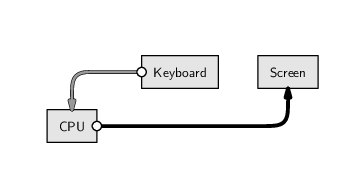
\includegraphics[width=0.5\linewidth]{img/script-commandline} \end{center}

\begin{center}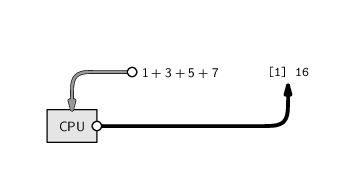
\includegraphics[width=0.5\linewidth]{img/script-commandlinedata} \end{center}

\begin{itemize}
\tightlist
\item
  Note que o resultado é apenas mostrado na tela, nada é salvo na
  memória (por enquanto)
\end{itemize}

\subsection{O editor de scripts}\label{o-editor-de-scripts}

\begin{itemize}
\tightlist
\item
  Para criar rotinas computacionais é necessário utilizar um editor de
  scripts.
\item
  Clique em
  \texttt{File\ \textgreater{}\ New\ file\ \textgreater{}\ R\ script}.
  Salve com a extensão \texttt{.R}.
\item
  Para enviar comandos diretamente para o console, selecione-os e aperte
  \texttt{Ctrl\ +\ \textless{}Enter\textgreater{}}.
\item
  Para adicionar comentários ao script, utiliza-se o símbolo \texttt{\#}
  antes do texto e/ou comandos. O que estiver depois do símbolo não será
  interpretado pelo R. Portanto:
\end{itemize}

\begin{Shaded}
\begin{Highlighting}[]
\DecValTok{2} \OperatorTok{+}\StringTok{ }\DecValTok{2}     \CommentTok{# esta linha será executada}
\CommentTok{# 2 + 2     esta linha não será executada}
\end{Highlighting}
\end{Shaded}

\subsection{Operadores aritméticos}\label{operadores-aritmeticos}

\begin{longtable}[]{@{}ll@{}}
\toprule
Operador & Significado\tabularnewline
\midrule
\endhead
\texttt{+} & adição\tabularnewline
\texttt{-} & subtração\tabularnewline
\texttt{*} & multiplicação\tabularnewline
\texttt{/} & divisão\tabularnewline
\texttt{\^{}} & potência\tabularnewline
\texttt{exp()} & exponencial\tabularnewline
\texttt{sqrt()} & raíz quadrada\tabularnewline
\texttt{factorial()} & fatorial\tabularnewline
\texttt{log()}; \texttt{log2()}; \texttt{log10()} &
logaritmos\tabularnewline
\bottomrule
\end{longtable}

\subsection{Ordens de execução}\label{ordens-de-execucao}

As operações são realizadas sempre seguindo as prioridades:

\begin{enumerate}
\def\labelenumi{\arabic{enumi}.}
\tightlist
\item
  De dentro para fora de parênteses \texttt{()}
\item
  Multiplicação e divisão
\item
  Adição e subtração
\end{enumerate}

\begin{Shaded}
\begin{Highlighting}[]
\OperatorTok{>}\StringTok{ }\DecValTok{5} \OperatorTok{*}\StringTok{ }\DecValTok{2} \OperatorTok{-}\StringTok{ }\DecValTok{10} \OperatorTok{+}\StringTok{ }\DecValTok{7}
\NormalTok{[}\DecValTok{1}\NormalTok{] }\DecValTok{7}
\OperatorTok{>}\StringTok{ }\DecValTok{5} \OperatorTok{*}\StringTok{ }\DecValTok{2} \OperatorTok{-}\StringTok{ }\NormalTok{(}\DecValTok{10} \OperatorTok{+}\StringTok{ }\DecValTok{7}\NormalTok{)}
\NormalTok{[}\DecValTok{1}\NormalTok{] }\OperatorTok{-}\DecValTok{7}
\OperatorTok{>}\StringTok{ }\DecValTok{5} \OperatorTok{*}\StringTok{ }\NormalTok{(}\DecValTok{2} \OperatorTok{-}\StringTok{ }\DecValTok{10} \OperatorTok{+}\StringTok{ }\DecValTok{7}\NormalTok{)}
\NormalTok{[}\DecValTok{1}\NormalTok{] }\OperatorTok{-}\DecValTok{5}
\OperatorTok{>}\StringTok{ }\DecValTok{5} \OperatorTok{*}\StringTok{ }\NormalTok{(}\DecValTok{2} \OperatorTok{-}\StringTok{ }\NormalTok{(}\DecValTok{10} \OperatorTok{+}\StringTok{ }\DecValTok{7}\NormalTok{))}
\NormalTok{[}\DecValTok{1}\NormalTok{] }\OperatorTok{-}\DecValTok{75}
\end{Highlighting}
\end{Shaded}

\subsection*{Exercícios}\label{exercicios}


\begin{enumerate}
\def\labelenumi{\arabic{enumi}.}
\tightlist
\item
  Calcule a seguinte equação: \(32 + 16^2 - 25^3\)
\item
  Divida o resultado por \(345\)
\item
  Qual o resultado da expressão \(\frac{e^{-2} 2^{4} - 1}{4!}\)?
\item
  E do logaritmo desta expressão?
\end{enumerate}

\subsection{\texorpdfstring{``Salvando''
resultados}{Salvando resultados}}\label{salvando-resultados}

Do exercício anterior

\begin{Shaded}
\begin{Highlighting}[]
\OperatorTok{>}\StringTok{ }\NormalTok{x <-}\StringTok{ }\DecValTok{32} \OperatorTok{+}\StringTok{ }\DecValTok{16}\OperatorTok{^}\DecValTok{2} \OperatorTok{-}\StringTok{ }\DecValTok{25}\OperatorTok{^}\DecValTok{3}
\OperatorTok{>}\StringTok{ }\NormalTok{x}
\NormalTok{[}\DecValTok{1}\NormalTok{] }\OperatorTok{-}\DecValTok{15337}
\OperatorTok{>}\StringTok{ }\NormalTok{x}\OperatorTok{/}\DecValTok{345}
\NormalTok{[}\DecValTok{1}\NormalTok{] }\OperatorTok{-}\FloatTok{44.45507}
\OperatorTok{>}\StringTok{ }\NormalTok{(y <-}\StringTok{ }\NormalTok{(}\KeywordTok{exp}\NormalTok{(}\OperatorTok{-}\DecValTok{2}\NormalTok{) }\OperatorTok{*}\StringTok{ }\DecValTok{2}\OperatorTok{^}\DecValTok{4} \OperatorTok{-}\StringTok{ }\DecValTok{1}\NormalTok{)}\OperatorTok{/}\KeywordTok{factorial}\NormalTok{(}\DecValTok{4}\NormalTok{))}
\NormalTok{[}\DecValTok{1}\NormalTok{] }\FloatTok{0.04855686}
\OperatorTok{>}\StringTok{ }\KeywordTok{log}\NormalTok{(y)}
\NormalTok{[}\DecValTok{1}\NormalTok{] }\OperatorTok{-}\FloatTok{3.02502}
\end{Highlighting}
\end{Shaded}

Quando criamos uma variável (\texttt{x}, \texttt{y}), ela fica
armazenada \textbf{temporariamente} na memória RAM.

\begin{center}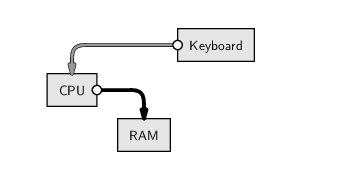
\includegraphics[width=0.5\linewidth]{img/script-assign} \end{center}

Para saber quais objetos estão criados, usamos a \textbf{função}
\texttt{ls()}

\begin{Shaded}
\begin{Highlighting}[]
\OperatorTok{>}\StringTok{ }\KeywordTok{ls}\NormalTok{()}
\NormalTok{[}\DecValTok{1}\NormalTok{] }\StringTok{"x"} \StringTok{"y"}
\end{Highlighting}
\end{Shaded}

Estas variáveis ficam armazenadas no chamado \emph{workspace} do R

\begin{itemize}
\tightlist
\item
  O \emph{workspace} consiste de tudo que or criado durante uma sessão
  do R, armazenado na memória RAM
\end{itemize}

Para efetivamente salvar esas variáveis, podemos armazenar esse
\emph{workspace} do R em disco, em um arquivo chamdo \texttt{.Rdata}

\begin{center}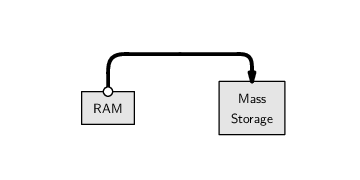
\includegraphics[width=0.5\linewidth]{img/script-workspace} \end{center}

\begin{center}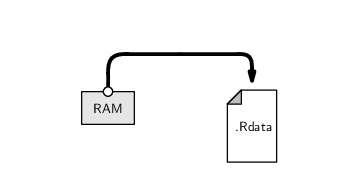
\includegraphics[width=0.5\linewidth]{img/script-workspacedata} \end{center}

\begin{itemize}
\tightlist
\item
  Quando o R é iniciado em um diretório com um arquivo \texttt{.Rdata},
  as variáveis salvas são automaticamente carregadas
\item
  No entanto, é sempre melhor salvar os dados e o \textbf{script}, assim
  é possível gerar os resultados novamente, sem salvar nada sem
  necessidade
\item
  Veremos mais pra frente como salvar variáveis específicas, por
  exemplo, resultados de uma análise que leva muito tempo para ser
  executada
\item
  O mais importante é salvar o \textbf{código}, assim sabemos
  \textbf{como} chegamos a determinado resultado, e podemos recriá-lo
  depois
\end{itemize}

\subsection{Finalizando o programa}\label{finalizando-o-programa}

A qualquer momento durante uma sessão você pode usar o comando

\begin{Shaded}
\begin{Highlighting}[]
\OperatorTok{>}\StringTok{ }\KeywordTok{save.image}\NormalTok{()}
\end{Highlighting}
\end{Shaded}

No RStudio:

\begin{itemize}
\tightlist
\item
  \texttt{File\ \textgreater{}\ Save\ As...}
\item
  Na janela que abrir, digite o nome do arquivo (por exemplo
  \texttt{script\_aula1}) e salve
\item
  Automaticamente o script será salvo com a extensão \texttt{.R} (nesse
  caso \texttt{script\_aula1.R}) no diretório de trabalho que você
  configurou no início
\end{itemize}

Alternativamente, você pode também salvar toda sua área de trabalho,
clicando em
\texttt{Workspace\ \textgreater{}\ Save\ As\ Default\ Workspace}. Este
processo irá gerar dois arquivos:

\begin{itemize}
\tightlist
\item
  \texttt{.Rdata}: contém todos os objetos criados durante uma sessão.
  Não é necessário (e nem recomendado) dar um nome antes do ponto. Dessa
  forma, a próxima vez que o programa for iniciado neste diretório, a
  área de trabalho será carregada automaticamente.
\item
  \texttt{.Rhistory}: um arquivo texto que contém todos os comandos que
  foram digitados no console.
\end{itemize}

\section*{Referências}\label{referencias}


\begin{itemize}
\tightlist
\item
  Leek, J. \href{https://leanpub.com/datastyle}{The Elements of Data
  Analytic Style}. Leanpub, 2015.
\item
  Murrell, P.
  \href{https://www.stat.auckland.ac.nz/~paul/ItDT/HTML}{Introduction to
  data technologies}. Boca Raton: Chapman \& Hall/CRC, 2009.
\item
  Peng, RD. \href{https://leanpub.com/rprogramming}{R programming for
  data science}. Leanpub, 2015.
\end{itemize}

\chapter{Objetos e classes}\label{objetos-e-classes}

\section{Funções e argumentos}\label{funcoes-e-argumentos}

As funções no R são definidas como:

\begin{Shaded}
\begin{Highlighting}[]
\KeywordTok{nome}\NormalTok{(argumento1, argumento2, ...)}
\end{Highlighting}
\end{Shaded}

Exemplo: função \texttt{runif()} (para gerar valores aleatórios de uma
distribuição uniforme):

\begin{Shaded}
\begin{Highlighting}[]
\KeywordTok{runif}\NormalTok{(n, }\DataTypeTok{min =} \DecValTok{0}\NormalTok{, }\DataTypeTok{max =} \DecValTok{1}\NormalTok{)}
\end{Highlighting}
\end{Shaded}

\begin{Shaded}
\begin{Highlighting}[]
\KeywordTok{runif}\NormalTok{(}\DecValTok{10}\NormalTok{, }\DecValTok{1}\NormalTok{, }\DecValTok{100}\NormalTok{)}
\NormalTok{ [}\DecValTok{1}\NormalTok{] }\FloatTok{31.468845} \FloatTok{26.509578} \FloatTok{55.679921}  \FloatTok{6.581932} \FloatTok{47.386379} \FloatTok{48.893303} \FloatTok{81.427859}
\NormalTok{ [}\DecValTok{8}\NormalTok{] }\FloatTok{37.661733} \FloatTok{55.109301} \FloatTok{17.855943}
\end{Highlighting}
\end{Shaded}

Argumentos que já possuem um valor especificado (como \texttt{max} e
\texttt{min}) podem ser omitidos:

\begin{Shaded}
\begin{Highlighting}[]
\KeywordTok{runif}\NormalTok{(}\DecValTok{10}\NormalTok{)}
\end{Highlighting}
\end{Shaded}

Se os argumentos forem nomeados, a ordem deles dentro da função não tem
mais importância:

\begin{Shaded}
\begin{Highlighting}[]
\KeywordTok{runif}\NormalTok{(}\DataTypeTok{min =} \DecValTok{1}\NormalTok{, }\DataTypeTok{max =} \DecValTok{100}\NormalTok{, }\DataTypeTok{n =} \DecValTok{10}\NormalTok{)}
\end{Highlighting}
\end{Shaded}

Argumentos nomeados e não nomeados podem ser utilizados, desde que os
não nomeados estejam na posição correta:

\begin{Shaded}
\begin{Highlighting}[]
\KeywordTok{runif}\NormalTok{(}\DecValTok{10}\NormalTok{, }\DataTypeTok{max =} \DecValTok{100}\NormalTok{, }\DataTypeTok{min =} \DecValTok{1}\NormalTok{)}
\end{Highlighting}
\end{Shaded}

\subsection{Outros tipos de
argumentos}\label{outros-tipos-de-argumentos}

Exemplo: função \texttt{sample()}:

\begin{Shaded}
\begin{Highlighting}[]
\KeywordTok{sample}\NormalTok{(x, size, }\DataTypeTok{replace =} \OtherTok{FALSE}\NormalTok{, }\DataTypeTok{prob =} \OtherTok{NULL}\NormalTok{)}
\end{Highlighting}
\end{Shaded}

\begin{itemize}
\tightlist
\item
  \texttt{x} e \texttt{size} devem ser obrigatoriamente especificados
\item
  \texttt{replace} é lógico: \texttt{TRUE} (\texttt{T}) ou
  \texttt{FALSE} (\texttt{F})
\item
  \texttt{prob} é um argumento vazio ou ausente (``opcional'')
\end{itemize}

Exemplo: função \texttt{plot()}:

\begin{Shaded}
\begin{Highlighting}[]
\KeywordTok{plot}\NormalTok{(x, y, ...)}
\end{Highlighting}
\end{Shaded}

\begin{itemize}
\tightlist
\item
  ``\texttt{...}'' permite especificar argumentos de outras funções (por
  exemplo \texttt{par()})
\end{itemize}

Para ver todos os argumentos disponíveis de uma função, podemos usar a
função \texttt{args()}

\begin{Shaded}
\begin{Highlighting}[]
\KeywordTok{args}\NormalTok{(sample)}
\ControlFlowTok{function}\NormalTok{ (x, size, }\DataTypeTok{replace =} \OtherTok{FALSE}\NormalTok{, }\DataTypeTok{prob =} \OtherTok{NULL}\NormalTok{) }
\OtherTok{NULL}
\end{Highlighting}
\end{Shaded}

\section{Mecanismos de ajuda}\label{mecanismos-de-ajuda}

Argumentos e detalhes do funcionamento das funções:

\begin{Shaded}
\begin{Highlighting}[]
\NormalTok{?runif}
\end{Highlighting}
\end{Shaded}

ou

\begin{Shaded}
\begin{Highlighting}[]
\KeywordTok{help}\NormalTok{(runif)}
\end{Highlighting}
\end{Shaded}

A documentação contém os campos:

\begin{itemize}
\tightlist
\item
  \textbf{Description:} breve descrição
\item
  \textbf{Usage:} função e todos seus argumentos
\item
  \textbf{Arguments:} lista descrevendo cada argumento
\item
  \textbf{Details:} descrição detalhada
\item
  \textbf{Value:} o que a função retorna
\item
  \textbf{References:} bibliografia relacionada
\item
  \textbf{See Also:} funções relacionadas
\item
  \textbf{Examples:} exemplos práticos
\end{itemize}

Procura por nomes de funções que contenham algum termo:

\begin{Shaded}
\begin{Highlighting}[]
\KeywordTok{apropos}\NormalTok{(}\StringTok{"mod"}\NormalTok{)}
\KeywordTok{apropos}\NormalTok{(}\StringTok{"model"}\NormalTok{)}
\end{Highlighting}
\end{Shaded}

Procura por funções que contenham \texttt{palavra} em qualquer parte de
sua documentação:

\begin{Shaded}
\begin{Highlighting}[]
\KeywordTok{help.search}\NormalTok{(}\StringTok{"palavra"}\NormalTok{)}
\end{Highlighting}
\end{Shaded}

Ajuda através do navegador (também contém manuais, \ldots{}):

\begin{Shaded}
\begin{Highlighting}[]
\KeywordTok{help.start}\NormalTok{()}
\end{Highlighting}
\end{Shaded}

Sites para busca na documentação dos diversos pacotes:

\begin{itemize}
\tightlist
\item
  RDocumentation \url{https://www.rdocumentation.org/}
\item
  R Package Documentation \url{https://rdrr.io/}
\item
  R Contributed Documentation (várias línguas)
  \url{https://cran.r-project.org/other-docs.html}
\end{itemize}

Os pacotes do R contém funções específicas para determinadas tarefas, e
estendem a instalação básica do R. Atualmente existem mais de 10000
pacotes disponíveis no
\href{http://cran-r.c3sl.ufpr.br/web/packages/index.html}{CRAN}, além de
diversos outros hospedados em sites como
\href{https://github.com}{Github}, por exemplo.

Ao instalar o R, os seguintes pacotes já vêm instalados (fazem parte do
chamado ``R core''):

\begin{verbatim}
NULL
\end{verbatim}

No entanto, nem todos são carregados na inicialização do R. Por padrão,
apenas os seguintes pacotes são carregados automaticamente:

\begin{verbatim}
[1] "knitr"     "stats"     "graphics"  "grDevices" "utils"     "datasets" 
[7] "methods"   "base"     
\end{verbatim}

Para listar os pacotes carregados, use a função

\begin{Shaded}
\begin{Highlighting}[]
\KeywordTok{search}\NormalTok{()}
\end{Highlighting}
\end{Shaded}

Note que o primeiro elemento, \texttt{.GlobalEnv}, será sempre carregado
pois ele é o \emph{ambiente} queirá armazenar (e deixar disponível) os
objetos criados pelo usuário. Para carregar um pacote instalado, usamos
a função \texttt{library()}, por exemplo

\begin{Shaded}
\begin{Highlighting}[]
\KeywordTok{library}\NormalTok{(lattice)}
\KeywordTok{search}\NormalTok{()}
\end{Highlighting}
\end{Shaded}

Isso tornará todas as funções do pacote \texttt{lattice} disponíveis
para uso.

Para instalar um pacote usamos a função \texttt{install.packages()}.
Sabendo o nome do pacote, por exemplo, \texttt{mvtnorm}, fazemos

\begin{Shaded}
\begin{Highlighting}[]
\KeywordTok{install.packages}\NormalTok{(}\StringTok{"mvtnorm"}\NormalTok{)}
\end{Highlighting}
\end{Shaded}

Se o diretório padrão de instalação de um pacote for de acesso restrito
(root por exemplo), o R irá perguntar se você gostaria de instalar o
pacote em uma biblioteca pessoal, e sugerirá um diretório que possui as
permissões necessárias. Você pode se antecipar e já definir e criar um
diretório na sua pasta pessoal, e instalar os pacotes sempre nesse
local. Por exemplo, defina \texttt{\textasciitilde{}/R/library} como sua
biblioteca pessoal. Para instalar os pacotes sempre nesse diretório
faça:

\begin{Shaded}
\begin{Highlighting}[]
\KeywordTok{install.packages}\NormalTok{(}\StringTok{"mvtnorm"}\NormalTok{, }\DataTypeTok{lib =} \StringTok{"~/R/library"}\NormalTok{)}
\end{Highlighting}
\end{Shaded}

Para verificar as bibliotecas disponíveis e se existem pacotes para ser
atualizados, use

\begin{Shaded}
\begin{Highlighting}[]
\KeywordTok{packageStatus}\NormalTok{()}
\end{Highlighting}
\end{Shaded}

Para atualizar automaticamente todos os pacotes faça

\begin{Shaded}
\begin{Highlighting}[]
\KeywordTok{update.packages}\NormalTok{(}\DataTypeTok{ask =} \OtherTok{FALSE}\NormalTok{)}
\end{Highlighting}
\end{Shaded}

\section{Criando uma função}\label{criando-uma-funcao}

A ideia original do R é transformar usuários em programadores

\begin{quote}
\emph{``\ldots{} to turn ideas into software, quickly and faithfully.''}

-- John M. Chambers
\end{quote}

Criar funções para realizar trabalhos específicos é um dos grandes
poderes do R

Por exemplo, podemos criar a famosa função

\begin{Shaded}
\begin{Highlighting}[]
\NormalTok{ola.mundo <-}\StringTok{ }\ControlFlowTok{function}\NormalTok{()\{}
    \KeywordTok{writeLines}\NormalTok{(}\StringTok{"Olá mundo"}\NormalTok{)}
\NormalTok{\}}
\end{Highlighting}
\end{Shaded}

E chama-la através de

\begin{Shaded}
\begin{Highlighting}[]
\KeywordTok{ola.mundo}\NormalTok{()}
\NormalTok{Olá mundo}
\end{Highlighting}
\end{Shaded}

A função acima não permite alterar o resultado de saída. Podemos fazer
isso incluindo um \textbf{argumento}

\begin{Shaded}
\begin{Highlighting}[]
\NormalTok{ola.mundo <-}\StringTok{ }\ControlFlowTok{function}\NormalTok{(texto)\{}
    \KeywordTok{writeLines}\NormalTok{(texto)}
\NormalTok{\}}
\end{Highlighting}
\end{Shaded}

E fazer por exemplo

\begin{Shaded}
\begin{Highlighting}[]
\KeywordTok{ola.mundo}\NormalTok{(}\StringTok{"Funções são legais"}\NormalTok{)}
\NormalTok{Funções são legais}
\end{Highlighting}
\end{Shaded}

(Veremos detalhes de funções mais adiante)

\section*{Exercícios}\label{exercicios-1}


\begin{enumerate}
\def\labelenumi{\arabic{enumi}.}
\tightlist
\item
  Usando a função \texttt{runif()} gere \(30\) números aleatórios entre:

  \begin{itemize}
  \tightlist
  \item
    0 e 1
  \item
    -5 e 5
  \item
    10 e 500
  \end{itemize}
\end{enumerate}

alternando a posição dos argumentos da função.

\begin{enumerate}
\def\labelenumi{\arabic{enumi}.}
\setcounter{enumi}{1}
\tightlist
\item
  Veja o help da função (?) \texttt{"+"}
\item
  Crie uma função para fazer a soma de dois números: \texttt{x} e
  \texttt{y}
\item
  Crie uma função para simular a jogada de um dado.
\item
  Crie uma função para simular a jogada de dois dados.
\end{enumerate}

\section{Objetos}\label{objetos}

O que é um objeto?

\begin{itemize}
\tightlist
\item
  Um \textbf{símbolo} ou uma \textbf{variável} capaz de armazenar
  qualquer valor ou estrutura de dados
\end{itemize}

Por quê objetos?

\begin{itemize}
\tightlist
\item
  Uma maneira simples de acessar os dados armazenados na memória (o R
  não permite acesso direto à memória)
\end{itemize}

Programação:

\begin{itemize}
\tightlist
\item
  Objetos \(\Rightarrow\) Classes \(\Rightarrow\) Métodos
\end{itemize}

\begin{quote}
\emph{``Tudo no R é um objeto.''}
\end{quote}

\begin{quote}
\emph{``Todo objeto no R tem uma classe''}
\end{quote}

\begin{itemize}
\tightlist
\item
  \textbf{Classe:} é a definição de um objeto. Descreve a forma do
  objeto e como ele será manipulado pelas diferentes funções
\item
  \textbf{Método:} são \textbf{funções genéricas} que executam suas
  tarefas de acordo com cada classe. Duas das funções genéricas mais
  importantes são:

  \begin{itemize}
  \tightlist
  \item
    \texttt{summary()}
  \item
    \texttt{plot()}
  \end{itemize}
\end{itemize}

Veja o resultado de

\begin{Shaded}
\begin{Highlighting}[]
\KeywordTok{methods}\NormalTok{(summary)}
\KeywordTok{methods}\NormalTok{(plot)}
\end{Highlighting}
\end{Shaded}

(Veremos mais detalhes adiante).

A variável \texttt{x} recebe o valor \(2\) (tornando-se um objeto dentro
do R):

\begin{Shaded}
\begin{Highlighting}[]
\NormalTok{x <-}\StringTok{ }\DecValTok{2}
\end{Highlighting}
\end{Shaded}

O símbolo \texttt{\textless{}-} é chamado de \textbf{operador de
atribuição}. Ele serve para atribuir valores a objetos, e é formado
pelos símbolos \texttt{\textless{}} e \texttt{-}, obrigatoriamente
\textbf{sem espaços}.

Para ver o conteúdo do objeto:

\begin{Shaded}
\begin{Highlighting}[]
\NormalTok{x}
\NormalTok{[}\DecValTok{1}\NormalTok{] }\DecValTok{2}
\end{Highlighting}
\end{Shaded}

\textbf{Observação}: O símbolo \texttt{=} pode ser usado no lugar de
\texttt{\textless{}-} mas não é recomendado.

Quando você faz

\begin{Shaded}
\begin{Highlighting}[]
\NormalTok{x <-}\StringTok{ }\DecValTok{2}
\end{Highlighting}
\end{Shaded}

está fazendo uma \textbf{declaração}, ou seja, declarando que a variável
\texttt{x} irá agora se tornar um objeto que armazena o número
\texttt{2}. As declarações podem ser feitas uma em cada linha

\begin{Shaded}
\begin{Highlighting}[]
\NormalTok{x <-}\StringTok{ }\DecValTok{2}
\NormalTok{y <-}\StringTok{ }\DecValTok{4}
\end{Highlighting}
\end{Shaded}

ou separadas por \texttt{;}

\begin{Shaded}
\begin{Highlighting}[]
\NormalTok{x <-}\StringTok{ }\DecValTok{2}\NormalTok{; y <-}\StringTok{ }\DecValTok{4}
\end{Highlighting}
\end{Shaded}

Operações matemáticas em objetos:

\begin{Shaded}
\begin{Highlighting}[]
\NormalTok{x }\OperatorTok{+}\StringTok{ }\NormalTok{x}
\NormalTok{[}\DecValTok{1}\NormalTok{] }\DecValTok{4}
\end{Highlighting}
\end{Shaded}

Objetos podem armazenar diferentes estruturas de dados:

\begin{Shaded}
\begin{Highlighting}[]
\NormalTok{y <-}\StringTok{ }\KeywordTok{runif}\NormalTok{(}\DecValTok{10}\NormalTok{)}
\NormalTok{y}
\NormalTok{ [}\DecValTok{1}\NormalTok{] }\FloatTok{0.6249965} \FloatTok{0.8821655} \FloatTok{0.2803538} \FloatTok{0.3984879} \FloatTok{0.7625511} \FloatTok{0.6690217} \FloatTok{0.2046122}
\NormalTok{ [}\DecValTok{8}\NormalTok{] }\FloatTok{0.3575249} \FloatTok{0.3594751} \FloatTok{0.6902905}
\end{Highlighting}
\end{Shaded}

Note que cada objeto só pode armazenar uma estrutura (um número ou uma
sequência de valores) de cada vez! (Aqui, o valor \(4\) que estava
armazenado em \texttt{y} foi sobrescrito pelos valores acima.)

\subsection{Nomes de objetos}\label{nomes-de-objetos}

\begin{itemize}
\tightlist
\item
  Podem ser formados por letras, números, ``\texttt{\_}'', e
  ``\texttt{.}''
\item
  Não podem começar com número e/ou ponto
\item
  Não podem conter espaços
\item
  Evite usar acentos
\item
  Evite usar nomes de funções como:
\end{itemize}

\texttt{c\ q\ t\ C\ D\ F\ I\ T\ diff\ df\ data\ var\ pt}

\begin{itemize}
\tightlist
\item
  O R é \emph{case-sensitive}, portanto:
\end{itemize}

\texttt{dados} \(\neq\) \texttt{Dados} \(\neq\) \texttt{DADOS}

\subsection{Gerenciando a área de
trabalho}\label{gerenciando-a-area-de-trabalho}

Liste os objetos criados com a função \texttt{ls()}:

\begin{Shaded}
\begin{Highlighting}[]
\KeywordTok{ls}\NormalTok{()}
\end{Highlighting}
\end{Shaded}

Para remover apenas um objeto:

\begin{Shaded}
\begin{Highlighting}[]
\KeywordTok{rm}\NormalTok{(x)}
\end{Highlighting}
\end{Shaded}

Para remover outros objetos:

\begin{Shaded}
\begin{Highlighting}[]
\KeywordTok{rm}\NormalTok{(x, y)}
\end{Highlighting}
\end{Shaded}

Para remover todos os objetos:

\begin{Shaded}
\begin{Highlighting}[]
\KeywordTok{rm}\NormalTok{(}\DataTypeTok{list =} \KeywordTok{ls}\NormalTok{())}
\end{Highlighting}
\end{Shaded}

\textbf{Cuidado!} O comando acima apaga todos os objetos na sua área de
trabalho sem perguntar. Depois só é possível recuperar os objetos ao
rodar os script novamente.

\section*{Exercícios}\label{exercicios-2}


\begin{enumerate}
\def\labelenumi{\arabic{enumi}.}
\tightlist
\item
  Armazene o resultado da equação \(32 + 16^2 - 25^3\) no objeto
  \texttt{x}
\item
  Divida \texttt{x} por \(345\) e armazene em \texttt{y}
\item
  Crie um objeto (com o nome que você quiser) para armazenar \(30\)
  valores aleatórios de uma distribuição uniforme entre \(10\) e \(50\)
\item
  Remova o objeto \texttt{y}
\item
  Remova os demais objetos de uma única vez
\item
  Procure a função utilizada para gerar numeros aleatórios de uma
  distribuição de Poisson, e gere \(100\) valores para a VA
  \(X \sim  \text{Poisson}(5)\).
\end{enumerate}

\section{Tipos e classes de objetos}\label{tipos-e-classes-de-objetos}

Para saber como trabalhar com dados no R, é fundamental entender as
possíveis estruturas (ou tipos) de dados possíveis. O formato mais
básico de dados são os vetores, e a partir deles, outras estruturas mais
complexas podem ser construídas. O R possui dois tipos básicos de
vetores:

\begin{itemize}
\tightlist
\item
  \textbf{Vetores atômicos}: existem seis tipos básicos:
\item
  \texttt{double}
\item
  \texttt{integer}
\item
  \texttt{character}
\item
  \texttt{logical}
\item
  \texttt{complex}
\item
  \texttt{raw}
\end{itemize}

Os tipos \texttt{integer} e \texttt{double} são chamados conjuntamente
de \texttt{numeric}. - \textbf{Listas}: também chamadas de \emph{vetores
recursivos} pois listas podem conter outras listas.

A principal diferença entre vetores atômicos e listas é que o primeiro é
\textbf{homogêneo} (cada vetor só pode conter um tipo), enquanto que o
segundo pode ser \textbf{heterogêneo} (cada vetor pode conter mais de um
tipo).

Um vetor atômico só pode conter elementos de um mesmo tipo

Um vetor, como o próprio nome diz, é uma estrutura unidimensional, mas
na maioria das vezes iremos trabalhar com estruturas de dados
bidimensionais (linhas e colunas). Portanto diferentes estruturas (com
diferentes dimensões) podem ser criadas a partir dos vetores atômicos.
Quando isso acontece, temos o que é chamado de \textbf{classe} de um
objeto. Embora os vetores atômicos só possuam seis tipos básicos, existe
um número muito grande de classes, e novas são inventadas todos os dias.
E mesmo que um objeto seja de qualquer classe, ele sempre será de um dos
seis tipos básicos (ou uma lista).

Para verificar o tipo de um objeto, usamos a função \texttt{typeof()},
enquanto que a classe é verificada com a função \texttt{class()}.
Vejamos alguns exemplos:

\begin{Shaded}
\begin{Highlighting}[]
\NormalTok{## double}
\NormalTok{x <-}\StringTok{ }\KeywordTok{c}\NormalTok{(}\DecValTok{2}\NormalTok{, }\DecValTok{4}\NormalTok{, }\DecValTok{6}\NormalTok{)}
\KeywordTok{typeof}\NormalTok{(x)}
\NormalTok{[}\DecValTok{1}\NormalTok{] }\StringTok{"double"}
\KeywordTok{class}\NormalTok{(x)}
\NormalTok{[}\DecValTok{1}\NormalTok{] }\StringTok{"numeric"}
\NormalTok{## integer}
\NormalTok{x <-}\StringTok{ }\KeywordTok{c}\NormalTok{(2L, 4L, 6L)}
\KeywordTok{typeof}\NormalTok{(x)}
\NormalTok{[}\DecValTok{1}\NormalTok{] }\StringTok{"integer"}
\KeywordTok{class}\NormalTok{(x)}
\NormalTok{[}\DecValTok{1}\NormalTok{] }\StringTok{"integer"}
\NormalTok{## character}
\NormalTok{x <-}\StringTok{ }\KeywordTok{c}\NormalTok{(}\StringTok{"a"}\NormalTok{, }\StringTok{"b"}\NormalTok{, }\StringTok{"c"}\NormalTok{)}
\KeywordTok{typeof}\NormalTok{(x)}
\NormalTok{[}\DecValTok{1}\NormalTok{] }\StringTok{"character"}
\KeywordTok{class}\NormalTok{(x)}
\NormalTok{[}\DecValTok{1}\NormalTok{] }\StringTok{"character"}
\NormalTok{## logical}
\NormalTok{x <-}\StringTok{ }\KeywordTok{c}\NormalTok{(}\OtherTok{TRUE}\NormalTok{, }\OtherTok{FALSE}\NormalTok{, }\OtherTok{TRUE}\NormalTok{)}
\KeywordTok{typeof}\NormalTok{(x)}
\NormalTok{[}\DecValTok{1}\NormalTok{] }\StringTok{"logical"}
\KeywordTok{class}\NormalTok{(x)}
\NormalTok{[}\DecValTok{1}\NormalTok{] }\StringTok{"logical"}
\NormalTok{## complex}
\NormalTok{x <-}\StringTok{ }\KeywordTok{c}\NormalTok{(}\DecValTok{2} \OperatorTok{+}\StringTok{ }\NormalTok{1i, }\DecValTok{4} \OperatorTok{+}\StringTok{ }\NormalTok{1i, }\DecValTok{6} \OperatorTok{+}\StringTok{ }\NormalTok{1i)}
\KeywordTok{typeof}\NormalTok{(x)}
\NormalTok{[}\DecValTok{1}\NormalTok{] }\StringTok{"complex"}
\KeywordTok{class}\NormalTok{(x)}
\NormalTok{[}\DecValTok{1}\NormalTok{] }\StringTok{"complex"}
\NormalTok{## raw}
\NormalTok{x <-}\StringTok{ }\KeywordTok{raw}\NormalTok{(}\DecValTok{3}\NormalTok{)}
\KeywordTok{typeof}\NormalTok{(x)}
\NormalTok{[}\DecValTok{1}\NormalTok{] }\StringTok{"raw"}
\KeywordTok{class}\NormalTok{(x)}
\NormalTok{[}\DecValTok{1}\NormalTok{] }\StringTok{"raw"}
\end{Highlighting}
\end{Shaded}

\subsection{Vetores numéricos}\label{vetores-numericos}

Características:

\begin{itemize}
\tightlist
\item
  Coleção ordenada de valores
\item
  Estrutura unidimensional
\end{itemize}

Usando a função \texttt{c()} para criar vetores:

\begin{Shaded}
\begin{Highlighting}[]
\NormalTok{num <-}\StringTok{ }\KeywordTok{c}\NormalTok{(}\DecValTok{10}\NormalTok{, }\DecValTok{5}\NormalTok{, }\DecValTok{2}\NormalTok{, }\DecValTok{4}\NormalTok{, }\DecValTok{8}\NormalTok{, }\DecValTok{9}\NormalTok{)}
\NormalTok{num}
\NormalTok{[}\DecValTok{1}\NormalTok{] }\DecValTok{10}  \DecValTok{5}  \DecValTok{2}  \DecValTok{4}  \DecValTok{8}  \DecValTok{9}
\KeywordTok{typeof}\NormalTok{(num)}
\NormalTok{[}\DecValTok{1}\NormalTok{] }\StringTok{"double"}
\KeywordTok{class}\NormalTok{(num)}
\NormalTok{[}\DecValTok{1}\NormalTok{] }\StringTok{"numeric"}
\end{Highlighting}
\end{Shaded}

Por que \texttt{numeric} e não \texttt{integer}?

\begin{Shaded}
\begin{Highlighting}[]
\NormalTok{x <-}\StringTok{ }\KeywordTok{c}\NormalTok{(10L, 5L, 2L, 4L, 8L, 9L)}
\NormalTok{x}
\NormalTok{[}\DecValTok{1}\NormalTok{] }\DecValTok{10}  \DecValTok{5}  \DecValTok{2}  \DecValTok{4}  \DecValTok{8}  \DecValTok{9}
\KeywordTok{typeof}\NormalTok{(x)}
\NormalTok{[}\DecValTok{1}\NormalTok{] }\StringTok{"integer"}
\KeywordTok{class}\NormalTok{(x)}
\NormalTok{[}\DecValTok{1}\NormalTok{] }\StringTok{"integer"}
\end{Highlighting}
\end{Shaded}

Para forçar a representação de um número para inteiro é necessário usar
o sufixo \texttt{L}.

Note que a diferença entre \texttt{numeric} e \texttt{integer} também
possui impacto computacional, pois o armazenamento de números inteiros
ocupa menos espaço na memória. Dessa forma, esperamos que o vetor
\texttt{x} acima ocupe menos espaço na memória do que o vetor
\texttt{num}, embora sejam aparentemente idênticos. Veja:

\begin{Shaded}
\begin{Highlighting}[]
\KeywordTok{object.size}\NormalTok{(num)}
\NormalTok{[}\DecValTok{1}\NormalTok{] }\DecValTok{96}\NormalTok{ bytes}
\KeywordTok{object.size}\NormalTok{(x)}
\NormalTok{[}\DecValTok{1}\NormalTok{] }\DecValTok{80}\NormalTok{ bytes}
\end{Highlighting}
\end{Shaded}

A diferença pode parecer pequena, mas pode ter um grande impacto
computacional quando os vetores são formados por milhares ou milhões de
números.

\subsubsection{Representação numérica dentro do
R}\label{representacao-numerica-dentro-do-r}

Os números que aparecem na tela do console do R são apenas
representações simplificadas do número real armazenado na memória. Por
exemplo,

\begin{Shaded}
\begin{Highlighting}[]
\NormalTok{x <-}\StringTok{ }\KeywordTok{runif}\NormalTok{(}\DecValTok{10}\NormalTok{)}
\NormalTok{x}
\NormalTok{ [}\DecValTok{1}\NormalTok{] }\FloatTok{0.2875775} \FloatTok{0.7883051} \FloatTok{0.4089769} \FloatTok{0.8830174} \FloatTok{0.9404673} \FloatTok{0.0455565} \FloatTok{0.5281055}
\NormalTok{ [}\DecValTok{8}\NormalTok{] }\FloatTok{0.8924190} \FloatTok{0.5514350} \FloatTok{0.4566147}
\end{Highlighting}
\end{Shaded}

O objeto \texttt{x} contém números como 0.2875775, 0.7883051, etc, que
possuem 7 casas decimais, que é o padrão do R. O número de casas
decimais é controlado pelo argumento \texttt{digits} da função
\texttt{options()}. Para visualizar essa opção, use

\begin{Shaded}
\begin{Highlighting}[]
\KeywordTok{getOption}\NormalTok{(}\StringTok{"digits"}\NormalTok{)}
\NormalTok{[}\DecValTok{1}\NormalTok{] }\DecValTok{7}
\end{Highlighting}
\end{Shaded}

Note que esse valor de 7 é o número de \textbf{dígitos significativos},
e pode variar conforme a sequência de números. Por exemplo,

\begin{Shaded}
\begin{Highlighting}[]
\NormalTok{y <-}\StringTok{ }\KeywordTok{runif}\NormalTok{(}\DecValTok{10}\NormalTok{)}
\NormalTok{y}
\NormalTok{ [}\DecValTok{1}\NormalTok{] }\FloatTok{0.069360916} \FloatTok{0.817775199} \FloatTok{0.942621732} \FloatTok{0.269381876} \FloatTok{0.169348123}
\NormalTok{ [}\DecValTok{6}\NormalTok{] }\FloatTok{0.033895622} \FloatTok{0.178785004} \FloatTok{0.641665366} \FloatTok{0.022877743} \FloatTok{0.008324827}
\end{Highlighting}
\end{Shaded}

possui valores com 9 casas decimais. Isto é apenas a representação do
número que aparece na tela. Internamente, cada número é armazenado com
uma precisão de 64 bits. Como consequência, cada número possui uma
acurácia de até 16 dígitos significativos. Isso pode introduzir algum
tipo de erro, por exemplo:

\begin{Shaded}
\begin{Highlighting}[]
\KeywordTok{sqrt}\NormalTok{(}\DecValTok{2}\NormalTok{)}\OperatorTok{^}\DecValTok{2} \OperatorTok{-}\StringTok{ }\DecValTok{2}
\NormalTok{[}\DecValTok{1}\NormalTok{] }\FloatTok{4.440892e-16}
\KeywordTok{print}\NormalTok{(}\KeywordTok{sqrt}\NormalTok{(}\DecValTok{2}\NormalTok{)}\OperatorTok{^}\DecValTok{2}\NormalTok{, }\DataTypeTok{digits =} \DecValTok{22}\NormalTok{)}
\NormalTok{[}\DecValTok{1}\NormalTok{] }\FloatTok{2.000000000000000444089}
\end{Highlighting}
\end{Shaded}

não é exatamente zero, pois a raíz quadrada de 2 não pode ser armazenada
com toda precisão com ``apenas'' 16 dígitos significativos. Esse tipo de
erro é chamado de \textbf{erro de ponto flutuante}, e as operações
nessas condições são chamadas de \textbf{aritmética de ponto flutuante}.
Para mais informações sobre esse assunto veja
\href{http://www.validlab.com/goldberg/paper.pdf}{What Every Computer
Scientist Should Know About Floating-Point Arithmetic} e
\href{http://cran-r.c3sl.ufpr.br/doc/FAQ/R-FAQ.html\#Why-doesn_0027t-R-think-these-numbers-are-equal_003f}{Why
doesn't R think these numbers are equal?}.

No R os números podem ser representados com até 22 casas decimais. Você
pode ver o número com toda sua precisão usando a função \texttt{print()}
e especificando o número de casas decimais com o argumento
\texttt{digits} (de 1 a 22)

\begin{Shaded}
\begin{Highlighting}[]
\KeywordTok{print}\NormalTok{(x, }\DataTypeTok{digits =} \DecValTok{1}\NormalTok{)}
\NormalTok{ [}\DecValTok{1}\NormalTok{] }\FloatTok{0.29} \FloatTok{0.79} \FloatTok{0.41} \FloatTok{0.88} \FloatTok{0.94} \FloatTok{0.05} \FloatTok{0.53} \FloatTok{0.89} \FloatTok{0.55} \FloatTok{0.46}
\KeywordTok{print}\NormalTok{(x, }\DataTypeTok{digits =} \DecValTok{7}\NormalTok{) }\CommentTok{# padrão}
\NormalTok{ [}\DecValTok{1}\NormalTok{] }\FloatTok{0.2875775} \FloatTok{0.7883051} \FloatTok{0.4089769} \FloatTok{0.8830174} \FloatTok{0.9404673} \FloatTok{0.0455565} \FloatTok{0.5281055}
\NormalTok{ [}\DecValTok{8}\NormalTok{] }\FloatTok{0.8924190} \FloatTok{0.5514350} \FloatTok{0.4566147}
\KeywordTok{print}\NormalTok{(x, }\DataTypeTok{digits =} \DecValTok{22}\NormalTok{)}
\NormalTok{ [}\DecValTok{1}\NormalTok{] }\FloatTok{0.28757752012461423873901} \FloatTok{0.78830513544380664825439}
\NormalTok{ [}\DecValTok{3}\NormalTok{] }\FloatTok{0.40897692181169986724854} \FloatTok{0.88301740400493144989014}
\NormalTok{ [}\DecValTok{5}\NormalTok{] }\FloatTok{0.94046728429384529590607} \FloatTok{0.04555649938993155956268}
\NormalTok{ [}\DecValTok{7}\NormalTok{] }\FloatTok{0.52810548804700374603271} \FloatTok{0.89241904439404606819153}
\NormalTok{ [}\DecValTok{9}\NormalTok{] }\FloatTok{0.55143501446582376956940} \FloatTok{0.45661473530344665050507}
\end{Highlighting}
\end{Shaded}

Também é possível alterar a representação na tela para o formato
científico, usando a função \texttt{format()}

\begin{Shaded}
\begin{Highlighting}[]
\KeywordTok{format}\NormalTok{(x, }\DataTypeTok{scientific =} \OtherTok{TRUE}\NormalTok{)}
\NormalTok{ [}\DecValTok{1}\NormalTok{] }\StringTok{"2.875775e-01"} \StringTok{"7.883051e-01"} \StringTok{"4.089769e-01"} \StringTok{"8.830174e-01"}
\NormalTok{ [}\DecValTok{5}\NormalTok{] }\StringTok{"9.404673e-01"} \StringTok{"4.555650e-02"} \StringTok{"5.281055e-01"} \StringTok{"8.924190e-01"}
\NormalTok{ [}\DecValTok{9}\NormalTok{] }\StringTok{"5.514350e-01"} \StringTok{"4.566147e-01"}
\end{Highlighting}
\end{Shaded}

Nessa representação, o valor 2.875775e-01 = \(2.875775 \times 10^{-01}\)
= \(0.2875775\).

\subsubsection{Sequências de números}\label{sequencias-de-numeros}

Usando a função \texttt{seq()}

\begin{Shaded}
\begin{Highlighting}[]
\KeywordTok{seq}\NormalTok{(}\DecValTok{1}\NormalTok{, }\DecValTok{10}\NormalTok{)}
\NormalTok{ [}\DecValTok{1}\NormalTok{]  }\DecValTok{1}  \DecValTok{2}  \DecValTok{3}  \DecValTok{4}  \DecValTok{5}  \DecValTok{6}  \DecValTok{7}  \DecValTok{8}  \DecValTok{9} \DecValTok{10}
\end{Highlighting}
\end{Shaded}

Ou \texttt{1:10} gera o mesmo resultado. Para a sequência variar em
\(2\)

\begin{Shaded}
\begin{Highlighting}[]
\KeywordTok{seq}\NormalTok{(}\DataTypeTok{from =} \DecValTok{1}\NormalTok{, }\DataTypeTok{to =} \DecValTok{10}\NormalTok{, }\DataTypeTok{by =} \DecValTok{2}\NormalTok{)}
\NormalTok{[}\DecValTok{1}\NormalTok{] }\DecValTok{1} \DecValTok{3} \DecValTok{5} \DecValTok{7} \DecValTok{9}
\end{Highlighting}
\end{Shaded}

Para obter \(15\) valores entre \(1\) e \(10\)

\begin{Shaded}
\begin{Highlighting}[]
\KeywordTok{seq}\NormalTok{(}\DataTypeTok{from =} \DecValTok{1}\NormalTok{, }\DataTypeTok{to =} \DecValTok{10}\NormalTok{, }\DataTypeTok{length.out =} \DecValTok{15}\NormalTok{)}
\NormalTok{ [}\DecValTok{1}\NormalTok{]  }\FloatTok{1.000000}  \FloatTok{1.642857}  \FloatTok{2.285714}  \FloatTok{2.928571}  \FloatTok{3.571429}  \FloatTok{4.214286}  \FloatTok{4.857143}
\NormalTok{ [}\DecValTok{8}\NormalTok{]  }\FloatTok{5.500000}  \FloatTok{6.142857}  \FloatTok{6.785714}  \FloatTok{7.428571}  \FloatTok{8.071429}  \FloatTok{8.714286}  \FloatTok{9.357143}
\NormalTok{[}\DecValTok{15}\NormalTok{] }\FloatTok{10.000000}
\end{Highlighting}
\end{Shaded}

Usando a função \texttt{rep()}

\begin{Shaded}
\begin{Highlighting}[]
\KeywordTok{rep}\NormalTok{(}\DecValTok{1}\NormalTok{, }\DecValTok{10}\NormalTok{)}
\NormalTok{ [}\DecValTok{1}\NormalTok{] }\DecValTok{1} \DecValTok{1} \DecValTok{1} \DecValTok{1} \DecValTok{1} \DecValTok{1} \DecValTok{1} \DecValTok{1} \DecValTok{1} \DecValTok{1}
\end{Highlighting}
\end{Shaded}

Para gerar um sequência várias vezes

\begin{Shaded}
\begin{Highlighting}[]
\KeywordTok{rep}\NormalTok{(}\KeywordTok{c}\NormalTok{(}\DecValTok{1}\NormalTok{, }\DecValTok{2}\NormalTok{, }\DecValTok{3}\NormalTok{), }\DataTypeTok{times =} \DecValTok{5}\NormalTok{)}
\NormalTok{ [}\DecValTok{1}\NormalTok{] }\DecValTok{1} \DecValTok{2} \DecValTok{3} \DecValTok{1} \DecValTok{2} \DecValTok{3} \DecValTok{1} \DecValTok{2} \DecValTok{3} \DecValTok{1} \DecValTok{2} \DecValTok{3} \DecValTok{1} \DecValTok{2} \DecValTok{3}
\end{Highlighting}
\end{Shaded}

Para repetir um número da sequência várias vezes

\begin{Shaded}
\begin{Highlighting}[]
\KeywordTok{rep}\NormalTok{(}\KeywordTok{c}\NormalTok{(}\DecValTok{1}\NormalTok{, }\DecValTok{2}\NormalTok{, }\DecValTok{3}\NormalTok{), }\DataTypeTok{each =} \DecValTok{5}\NormalTok{)}
\NormalTok{ [}\DecValTok{1}\NormalTok{] }\DecValTok{1} \DecValTok{1} \DecValTok{1} \DecValTok{1} \DecValTok{1} \DecValTok{2} \DecValTok{2} \DecValTok{2} \DecValTok{2} \DecValTok{2} \DecValTok{3} \DecValTok{3} \DecValTok{3} \DecValTok{3} \DecValTok{3}
\end{Highlighting}
\end{Shaded}

\subsubsection{Operações matemáticas em vetores
numéricos}\label{operacoes-matematicas-em-vetores-numericos}

Operações podem ser feitas entre um vetor e um número:

\begin{Shaded}
\begin{Highlighting}[]
\NormalTok{num }\OperatorTok{*}\StringTok{ }\DecValTok{2}
\NormalTok{[}\DecValTok{1}\NormalTok{] }\DecValTok{20} \DecValTok{10}  \DecValTok{4}  \DecValTok{8} \DecValTok{16} \DecValTok{18}
\end{Highlighting}
\end{Shaded}

E também entre vetores de mesmo comprimento ou com comprimentos
múltiplos:

\begin{Shaded}
\begin{Highlighting}[]
\NormalTok{num }\OperatorTok{*}\StringTok{ }\NormalTok{num}
\NormalTok{[}\DecValTok{1}\NormalTok{] }\DecValTok{100}  \DecValTok{25}   \DecValTok{4}  \DecValTok{16}  \DecValTok{64}  \DecValTok{81}
\NormalTok{num }\OperatorTok{+}\StringTok{ }\KeywordTok{c}\NormalTok{(}\DecValTok{2}\NormalTok{, }\DecValTok{4}\NormalTok{, }\DecValTok{1}\NormalTok{)}
\NormalTok{[}\DecValTok{1}\NormalTok{] }\DecValTok{12}  \DecValTok{9}  \DecValTok{3}  \DecValTok{6} \DecValTok{12} \DecValTok{10}
\end{Highlighting}
\end{Shaded}

\subsubsection{A Regra da Reciclagem}\label{a-regra-da-reciclagem}

\begin{center}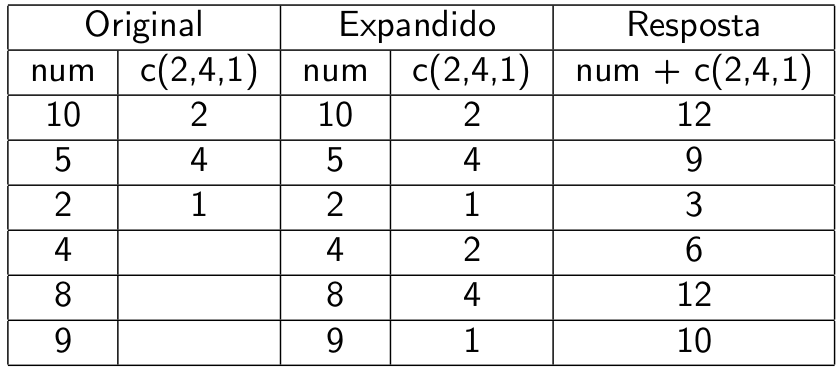
\includegraphics[width=0.8\linewidth]{img/reciclagem} \end{center}

Agora tente:

\begin{Shaded}
\begin{Highlighting}[]
\NormalTok{num }\OperatorTok{+}\StringTok{ }\KeywordTok{c}\NormalTok{(}\DecValTok{2}\NormalTok{, }\DecValTok{4}\NormalTok{, }\DecValTok{1}\NormalTok{, }\DecValTok{3}\NormalTok{)}
\end{Highlighting}
\end{Shaded}

\subsection{Outros tipos de vetores}\label{outros-tipos-de-vetores}

Vetores também podem ter outros tipos:

\begin{itemize}
\tightlist
\item
  Vetor de caracteres:
\end{itemize}

\begin{Shaded}
\begin{Highlighting}[]
\NormalTok{caracter <-}\StringTok{ }\KeywordTok{c}\NormalTok{(}\StringTok{"brava"}\NormalTok{, }\StringTok{"joaquina"}\NormalTok{, }\StringTok{"armação"}\NormalTok{)}
\NormalTok{caracter}
\NormalTok{[}\DecValTok{1}\NormalTok{] }\StringTok{"brava"}    \StringTok{"joaquina"} \StringTok{"armação"} 
\KeywordTok{typeof}\NormalTok{(caracter)}
\NormalTok{[}\DecValTok{1}\NormalTok{] }\StringTok{"character"}
\KeywordTok{class}\NormalTok{(caracter)}
\NormalTok{[}\DecValTok{1}\NormalTok{] }\StringTok{"character"}
\end{Highlighting}
\end{Shaded}

\begin{itemize}
\tightlist
\item
  Vetor lógico:
\end{itemize}

\begin{Shaded}
\begin{Highlighting}[]
\NormalTok{logico <-}\StringTok{ }\NormalTok{caracter }\OperatorTok{==}\StringTok{ "armação"}
\NormalTok{logico}
\NormalTok{[}\DecValTok{1}\NormalTok{] }\OtherTok{FALSE} \OtherTok{FALSE}  \OtherTok{TRUE}
\KeywordTok{typeof}\NormalTok{(logico)}
\NormalTok{[}\DecValTok{1}\NormalTok{] }\StringTok{"logical"}
\KeywordTok{class}\NormalTok{(logico)}
\NormalTok{[}\DecValTok{1}\NormalTok{] }\StringTok{"logical"}
\end{Highlighting}
\end{Shaded}

ou

\begin{Shaded}
\begin{Highlighting}[]
\NormalTok{logico <-}\StringTok{ }\NormalTok{num }\OperatorTok{>}\StringTok{ }\DecValTok{4}
\NormalTok{logico}
\NormalTok{[}\DecValTok{1}\NormalTok{]  }\OtherTok{TRUE}  \OtherTok{TRUE} \OtherTok{FALSE} \OtherTok{FALSE}  \OtherTok{TRUE}  \OtherTok{TRUE}
\end{Highlighting}
\end{Shaded}

No exemplo anterior, a condição \texttt{num\ \textgreater{}\ 4} é uma
\textbf{expressão condicional}, e o símbolo \texttt{\textgreater{}} um
\textbf{operador lógico}. Os operadores lógicos utilizados no R são:

\begin{longtable}[]{@{}cll@{}}
\toprule
Operador & Sintaxe & Teste\tabularnewline
\midrule
\endhead
\texttt{\textless{}} & \texttt{a\ \textless{}\ b} & \texttt{a} é menor
que \texttt{b}?\tabularnewline
\texttt{\textless{}=} & \texttt{a\ \textless{}=\ b} & \texttt{a} é menor
ou igual a \texttt{b}?\tabularnewline
\texttt{\textgreater{}} & \texttt{a\ \textgreater{}\ b} & \texttt{a} é
maior que \texttt{b}\tabularnewline
\texttt{\textgreater{}=} & \texttt{a\ \textgreater{}=\ b} & \texttt{a} é
maior ou igual a \texttt{b}?\tabularnewline
\texttt{==} & \texttt{a\ ==\ b} & \texttt{a} é igual a
\texttt{b}?\tabularnewline
\texttt{!=} & \texttt{a\ !=\ b} & \texttt{a} é diferente de
\texttt{b}?\tabularnewline
\texttt{\%in\%} & \texttt{a\ \%in\%\ c(a,\ b)} & \texttt{a} está contido
no vetor \texttt{c(a,\ b)}?\tabularnewline
\bottomrule
\end{longtable}

\subsection{Misturando classes de
objetos}\label{misturando-classes-de-objetos}

Algumas vezes isso acontece por acidente, mas também pode acontecer de
propósito.

O que acontece aqui?

\begin{Shaded}
\begin{Highlighting}[]
\NormalTok{w <-}\StringTok{ }\KeywordTok{c}\NormalTok{(5L, }\StringTok{"a"}\NormalTok{)}
\NormalTok{x <-}\StringTok{ }\KeywordTok{c}\NormalTok{(}\FloatTok{1.7}\NormalTok{, }\StringTok{"a"}\NormalTok{)}
\NormalTok{y <-}\StringTok{ }\KeywordTok{c}\NormalTok{(}\OtherTok{TRUE}\NormalTok{, }\DecValTok{2}\NormalTok{)}
\NormalTok{z <-}\StringTok{ }\KeywordTok{c}\NormalTok{(}\StringTok{"a"}\NormalTok{, T)}
\end{Highlighting}
\end{Shaded}

Lembre-se da regra:

Um vetor só pode conter elementos do mesmo tipo

Quando objetos de diferentes tipos são misturados, ocorre a
\textbf{coerção}, para que cada elemento possua a mesma classe.

Nos exemplos acima, nós vemos o efeito da \textbf{coerção implícita},
quando o R tenta representar todos os objetos de uma única forma.

Nós podemos forçar um objeto a mudar de classe, através da
\textbf{coerção explícita}, realizada pelas funções \texttt{as.*}:

\begin{Shaded}
\begin{Highlighting}[]
\NormalTok{x <-}\StringTok{ }\DecValTok{0}\OperatorTok{:}\DecValTok{6}
\KeywordTok{typeof}\NormalTok{(x)}
\NormalTok{[}\DecValTok{1}\NormalTok{] }\StringTok{"integer"}
\KeywordTok{class}\NormalTok{(x)}
\NormalTok{[}\DecValTok{1}\NormalTok{] }\StringTok{"integer"}
\KeywordTok{as.numeric}\NormalTok{(x)}
\NormalTok{[}\DecValTok{1}\NormalTok{] }\DecValTok{0} \DecValTok{1} \DecValTok{2} \DecValTok{3} \DecValTok{4} \DecValTok{5} \DecValTok{6}
\KeywordTok{as.logical}\NormalTok{(x)}
\NormalTok{[}\DecValTok{1}\NormalTok{] }\OtherTok{FALSE}  \OtherTok{TRUE}  \OtherTok{TRUE}  \OtherTok{TRUE}  \OtherTok{TRUE}  \OtherTok{TRUE}  \OtherTok{TRUE}
\KeywordTok{as.character}\NormalTok{(x)}
\NormalTok{[}\DecValTok{1}\NormalTok{] }\StringTok{"0"} \StringTok{"1"} \StringTok{"2"} \StringTok{"3"} \StringTok{"4"} \StringTok{"5"} \StringTok{"6"}
\KeywordTok{as.factor}\NormalTok{(x)}
\NormalTok{[}\DecValTok{1}\NormalTok{] }\DecValTok{0} \DecValTok{1} \DecValTok{2} \DecValTok{3} \DecValTok{4} \DecValTok{5} \DecValTok{6}
\NormalTok{Levels}\OperatorTok{:}\StringTok{ }\DecValTok{0} \DecValTok{1} \DecValTok{2} \DecValTok{3} \DecValTok{4} \DecValTok{5} \DecValTok{6}
\end{Highlighting}
\end{Shaded}

De \texttt{?logical}:

\begin{verbatim}
 Logical vectors are coerced to integer vectors in contexts where a
 numerical value is required, with ‘TRUE’ being mapped to ‘1L’,
 ‘FALSE’ to ‘0L’ and ‘NA’ to ‘NA_integer_’.
\end{verbatim}

\begin{Shaded}
\begin{Highlighting}[]
\NormalTok{(x <-}\StringTok{ }\KeywordTok{c}\NormalTok{(}\OtherTok{FALSE}\NormalTok{, }\OtherTok{TRUE}\NormalTok{))}
\NormalTok{[}\DecValTok{1}\NormalTok{] }\OtherTok{FALSE}  \OtherTok{TRUE}
\KeywordTok{class}\NormalTok{(x)}
\NormalTok{[}\DecValTok{1}\NormalTok{] }\StringTok{"logical"}
\KeywordTok{as.numeric}\NormalTok{(x)}
\NormalTok{[}\DecValTok{1}\NormalTok{] }\DecValTok{0} \DecValTok{1}
\end{Highlighting}
\end{Shaded}

Algumas vezes não é possível fazer a coerção, então:

\begin{Shaded}
\begin{Highlighting}[]
\NormalTok{x <-}\StringTok{ }\KeywordTok{c}\NormalTok{(}\StringTok{"a"}\NormalTok{, }\StringTok{"b"}\NormalTok{, }\StringTok{"c"}\NormalTok{)}
\KeywordTok{as.numeric}\NormalTok{(x)}
\NormalTok{Warning}\OperatorTok{:}\StringTok{ }\NormalTok{NAs introduced by coercion}
\NormalTok{[}\DecValTok{1}\NormalTok{] }\OtherTok{NA} \OtherTok{NA} \OtherTok{NA}
\KeywordTok{as.logical}\NormalTok{(x)}
\NormalTok{[}\DecValTok{1}\NormalTok{] }\OtherTok{NA} \OtherTok{NA} \OtherTok{NA}
\end{Highlighting}
\end{Shaded}

\subsection{Valores perdidos e
especiais}\label{valores-perdidos-e-especiais}

Valores perdidos devem ser definidos como \texttt{NA} (\emph{not
available}):

\begin{Shaded}
\begin{Highlighting}[]
\NormalTok{perd <-}\StringTok{ }\KeywordTok{c}\NormalTok{(}\DecValTok{3}\NormalTok{, }\DecValTok{5}\NormalTok{, }\OtherTok{NA}\NormalTok{, }\DecValTok{2}\NormalTok{)}
\NormalTok{perd}
\NormalTok{[}\DecValTok{1}\NormalTok{]  }\DecValTok{3}  \DecValTok{5} \OtherTok{NA}  \DecValTok{2}
\KeywordTok{class}\NormalTok{(perd)}
\NormalTok{[}\DecValTok{1}\NormalTok{] }\StringTok{"numeric"}
\end{Highlighting}
\end{Shaded}

Podemos testar a presença de \texttt{NA}s com a função \texttt{is.na()}:

\begin{Shaded}
\begin{Highlighting}[]
\KeywordTok{is.na}\NormalTok{(perd)}
\NormalTok{[}\DecValTok{1}\NormalTok{] }\OtherTok{FALSE} \OtherTok{FALSE}  \OtherTok{TRUE} \OtherTok{FALSE}
\end{Highlighting}
\end{Shaded}

Ou:

\begin{Shaded}
\begin{Highlighting}[]
\KeywordTok{any}\NormalTok{(}\KeywordTok{is.na}\NormalTok{(perd))}
\NormalTok{[}\DecValTok{1}\NormalTok{] }\OtherTok{TRUE}
\end{Highlighting}
\end{Shaded}

Outros valores especiais são:

\begin{itemize}
\tightlist
\item
  \texttt{NaN} (\emph{not a number}) - exemplo: \texttt{0/0}
\item
  \texttt{-Inf} e \texttt{Inf} - exemplo: \texttt{1/0}
\end{itemize}

A função \texttt{is.na()} também testa a presença de \texttt{NaN}s:

\begin{Shaded}
\begin{Highlighting}[]
\NormalTok{perd <-}\StringTok{ }\KeywordTok{c}\NormalTok{(}\OperatorTok{-}\DecValTok{1}\NormalTok{,}\DecValTok{0}\NormalTok{,}\DecValTok{1}\NormalTok{)}\OperatorTok{/}\DecValTok{0}
\NormalTok{perd}
\NormalTok{[}\DecValTok{1}\NormalTok{] }\OperatorTok{-}\OtherTok{Inf}  \OtherTok{NaN}  \OtherTok{Inf}
\KeywordTok{is.na}\NormalTok{(perd)}
\NormalTok{[}\DecValTok{1}\NormalTok{] }\OtherTok{FALSE}  \OtherTok{TRUE} \OtherTok{FALSE}
\end{Highlighting}
\end{Shaded}

A função \texttt{is.infinite()} testa se há valores infinitos

\begin{Shaded}
\begin{Highlighting}[]
\KeywordTok{is.infinite}\NormalTok{(perd)}
\NormalTok{[}\DecValTok{1}\NormalTok{]  }\OtherTok{TRUE} \OtherTok{FALSE}  \OtherTok{TRUE}
\end{Highlighting}
\end{Shaded}

\section*{Exercícios}\label{exercicios-3}


\begin{enumerate}
\def\labelenumi{\arabic{enumi}.}
\tightlist
\item
  Crie um objeto com os valores 54, 0, 17, 94, 12.5, 2, 0.9, 15.

  \begin{enumerate}
  \def\labelenumii{\alph{enumii}.}
  \tightlist
  \item
    Some o objeto acima com os valores 5, 6, e depois com os valores 5,
    6, 7.
  \end{enumerate}
\item
  Construa um único objeto com as letras: \texttt{A}, \texttt{B}, e
  \texttt{C}, repetidas cada uma 15, 12, e 8 vezes, respectivamente.

  \begin{enumerate}
  \def\labelenumii{\alph{enumii}.}
  \tightlist
  \item
    Mostre na tela, em forma de verdadeiro ou falso, onde estão as
    letras \texttt{B} nesse objeto.
  \item
    Veja a página de ajuda da função \texttt{sum()} e descubra como
    fazer para contar o número de letras \texttt{B} neste vetor (usando
    \texttt{sum()}).
  \end{enumerate}
\item
  Crie um objeto com 100 valores aleatórios de uma distribuição uniforme
  \(U(0,1)\). Conte quantas vezes aparecem valores maiores ou iguais a
  0,5.
\item
  Calcule as 50 primeiras potências de 2, ou seja,
  \(2, 2^2, 2^3,  \ldots, 2^{50}\).

  \begin{enumerate}
  \def\labelenumii{\alph{enumii}.}
  \tightlist
  \item
    Calcule o quadrado dos números inteiros de 1 a 50, ou seja,
    \(1^2, 2^2, 3^2, \ldots, 50^2\).
  \item
    Quais pares são iguais, ou seja, quais números inteiros dos dois
    exercícios anteriores satisfazem a condição \(2^n = n^2\)?
  \item
    Quantos pares existem?
  \end{enumerate}
\item
  Calcule o seno, coseno e a tangente para os números variando de \(0\)
  a \(2\pi\), com distância de \(0.1\) entre eles. (Use as funções
  \texttt{sin()}, \texttt{cos()}, \texttt{tan()}).

  \begin{enumerate}
  \def\labelenumii{\alph{enumii}.}
  \tightlist
  \item
    Calcule a tangente usando a relação \(\tan(x) = \sin(x)/\cos(x)\).
  \item
    Calcule as diferenças das tangentes calculadas pela função do R e
    pela razão acima.
  \item
    Quais valores são exatamente iguais?
  \item
    Qual a diferença máxima (em módulo) entre eles? Qual é a causa dessa
    diferença?
  \end{enumerate}
\end{enumerate}

\section{Outras classes}\label{outras-classes}

Como mencionado na seção anterior, o R possui 6 tipos básicos de
estrutura de dados, mas diversas classes podem ser construídas a partir
destes tipos básicos. Abaixo, veremos algumas das mais importantes.

\subsection{Fator}\label{fator}

Os fatores são parecidos com caracteres no R, mas são armazenados e
tratados de maneira diferente.

Características:

\begin{itemize}
\tightlist
\item
  Coleção de categorias ou \textbf{níveis} (\emph{levels})
\item
  Estrutura unidimensional
\end{itemize}

Utilizando as funções \texttt{factor()} e \texttt{c()}:

\begin{Shaded}
\begin{Highlighting}[]
\NormalTok{fator <-}\StringTok{ }\KeywordTok{factor}\NormalTok{(}\KeywordTok{c}\NormalTok{(}\StringTok{"alta"}\NormalTok{,}\StringTok{"baixa"}\NormalTok{,}\StringTok{"baixa"}\NormalTok{,}\StringTok{"media"}\NormalTok{,}
                  \StringTok{"alta"}\NormalTok{,}\StringTok{"media"}\NormalTok{,}\StringTok{"baixa"}\NormalTok{,}\StringTok{"media"}\NormalTok{,}\StringTok{"media"}\NormalTok{))}
\NormalTok{fator}
\NormalTok{[}\DecValTok{1}\NormalTok{] alta  baixa baixa media alta  media baixa media media}
\NormalTok{Levels}\OperatorTok{:}\StringTok{ }\NormalTok{alta baixa media}
\KeywordTok{class}\NormalTok{(fator)}
\NormalTok{[}\DecValTok{1}\NormalTok{] }\StringTok{"factor"}
\KeywordTok{typeof}\NormalTok{(fator)}
\NormalTok{[}\DecValTok{1}\NormalTok{] }\StringTok{"integer"}
\end{Highlighting}
\end{Shaded}

Note que o objeto é da classe \texttt{factor}, mas seu tipo básico é
\texttt{integer}! Isso significa que cada categoria única é identificada
internamente por um número, e isso faz com que os fatores possuam uma
ordenação, de acordo com as categorias únicas. Por isso existe a
identificação dos \texttt{Levels} (níveis) de um fator.

Veja o que acontece quando ``remover a classe'' desse objeto

\begin{Shaded}
\begin{Highlighting}[]
\KeywordTok{unclass}\NormalTok{(fator)}
\NormalTok{[}\DecValTok{1}\NormalTok{] }\DecValTok{1} \DecValTok{2} \DecValTok{2} \DecValTok{3} \DecValTok{1} \DecValTok{3} \DecValTok{2} \DecValTok{3} \DecValTok{3}
\KeywordTok{attr}\NormalTok{(,}\StringTok{"levels"}\NormalTok{)}
\NormalTok{[}\DecValTok{1}\NormalTok{] }\StringTok{"alta"}  \StringTok{"baixa"} \StringTok{"media"}
\end{Highlighting}
\end{Shaded}

Fatores podem ser convertidos para caracteres, e \textbf{também} para
números inteiros

\begin{Shaded}
\begin{Highlighting}[]
\KeywordTok{as.character}\NormalTok{(fator)}
\NormalTok{[}\DecValTok{1}\NormalTok{] }\StringTok{"alta"}  \StringTok{"baixa"} \StringTok{"baixa"} \StringTok{"media"} \StringTok{"alta"}  \StringTok{"media"} \StringTok{"baixa"} \StringTok{"media"} \StringTok{"media"}
\KeywordTok{as.integer}\NormalTok{(fator)}
\NormalTok{[}\DecValTok{1}\NormalTok{] }\DecValTok{1} \DecValTok{2} \DecValTok{2} \DecValTok{3} \DecValTok{1} \DecValTok{3} \DecValTok{2} \DecValTok{3} \DecValTok{3}
\end{Highlighting}
\end{Shaded}

Caso haja uma hierarquia, os níveis dos fatores podem ser ordenados
explicitamente através do argumento \texttt{levels}:

\begin{Shaded}
\begin{Highlighting}[]
\NormalTok{fator <-}\StringTok{ }\KeywordTok{factor}\NormalTok{(}\KeywordTok{c}\NormalTok{(}\StringTok{"alta"}\NormalTok{,}\StringTok{"baixa"}\NormalTok{,}\StringTok{"baixa"}\NormalTok{,}\StringTok{"media"}\NormalTok{,}
                  \StringTok{"alta"}\NormalTok{,}\StringTok{"media"}\NormalTok{,}\StringTok{"baixa"}\NormalTok{,}\StringTok{"media"}\NormalTok{,}\StringTok{"media"}\NormalTok{),}
                \DataTypeTok{levels =} \KeywordTok{c}\NormalTok{(}\StringTok{"alta"}\NormalTok{,}\StringTok{"media"}\NormalTok{,}\StringTok{"baixa"}\NormalTok{))}
\NormalTok{fator}
\NormalTok{[}\DecValTok{1}\NormalTok{] alta  baixa baixa media alta  media baixa media media}
\NormalTok{Levels}\OperatorTok{:}\StringTok{ }\NormalTok{alta media baixa}
\KeywordTok{typeof}\NormalTok{(fator)}
\NormalTok{[}\DecValTok{1}\NormalTok{] }\StringTok{"integer"}
\KeywordTok{class}\NormalTok{(fator)}
\NormalTok{[}\DecValTok{1}\NormalTok{] }\StringTok{"factor"}
\end{Highlighting}
\end{Shaded}

Além disso, os níveis dos fatores podem também ser explicitamente
ordenados

\begin{Shaded}
\begin{Highlighting}[]
\NormalTok{fator <-}\StringTok{ }\KeywordTok{factor}\NormalTok{(}\KeywordTok{c}\NormalTok{(}\StringTok{"alta"}\NormalTok{,}\StringTok{"baixa"}\NormalTok{,}\StringTok{"baixa"}\NormalTok{,}\StringTok{"media"}\NormalTok{,}
                  \StringTok{"alta"}\NormalTok{,}\StringTok{"media"}\NormalTok{,}\StringTok{"baixa"}\NormalTok{,}\StringTok{"media"}\NormalTok{,}\StringTok{"media"}\NormalTok{),}
                \DataTypeTok{levels =} \KeywordTok{c}\NormalTok{(}\StringTok{"baixa"}\NormalTok{, }\StringTok{"media"}\NormalTok{, }\StringTok{"alta"}\NormalTok{),}
                \DataTypeTok{ordered =} \OtherTok{TRUE}\NormalTok{)}
\NormalTok{fator}
\NormalTok{[}\DecValTok{1}\NormalTok{] alta  baixa baixa media alta  media baixa media media}
\NormalTok{Levels}\OperatorTok{:}\StringTok{ }\NormalTok{baixa }\OperatorTok{<}\StringTok{ }\NormalTok{media }\OperatorTok{<}\StringTok{ }\NormalTok{alta}
\KeywordTok{typeof}\NormalTok{(fator)}
\NormalTok{[}\DecValTok{1}\NormalTok{] }\StringTok{"integer"}
\KeywordTok{class}\NormalTok{(fator)}
\NormalTok{[}\DecValTok{1}\NormalTok{] }\StringTok{"ordered"} \StringTok{"factor"} 
\end{Highlighting}
\end{Shaded}

(Veja que um objeto pode ter mais de uma classe). Isso geralmente só
será útil em casos especificos.

As seguintes funções são úteis para verificar os níveis e o número de
níveis de um fator:

\begin{Shaded}
\begin{Highlighting}[]
\KeywordTok{levels}\NormalTok{(fator)}
\NormalTok{[}\DecValTok{1}\NormalTok{] }\StringTok{"baixa"} \StringTok{"media"} \StringTok{"alta"} 
\KeywordTok{nlevels}\NormalTok{(fator)}
\NormalTok{[}\DecValTok{1}\NormalTok{] }\DecValTok{3}
\end{Highlighting}
\end{Shaded}

\subsection{Matriz}\label{matriz}

Matrizes são vetores que podem ser dispostos em duas dimensões.

Características:

\begin{itemize}
\tightlist
\item
  Podem conter apenas um tipo de informação (números, caracteres)
\item
  Estrutura bidimensional
\end{itemize}

Utilizando a função \texttt{matrix()}:

\begin{Shaded}
\begin{Highlighting}[]
\NormalTok{matriz <-}\StringTok{ }\KeywordTok{matrix}\NormalTok{(}\DecValTok{1}\OperatorTok{:}\DecValTok{12}\NormalTok{, }\DataTypeTok{nrow =} \DecValTok{3}\NormalTok{, }\DataTypeTok{ncol =} \DecValTok{4}\NormalTok{)}
\NormalTok{matriz}
\NormalTok{     [,}\DecValTok{1}\NormalTok{] [,}\DecValTok{2}\NormalTok{] [,}\DecValTok{3}\NormalTok{] [,}\DecValTok{4}\NormalTok{]}
\NormalTok{[}\DecValTok{1}\NormalTok{,]    }\DecValTok{1}    \DecValTok{4}    \DecValTok{7}   \DecValTok{10}
\NormalTok{[}\DecValTok{2}\NormalTok{,]    }\DecValTok{2}    \DecValTok{5}    \DecValTok{8}   \DecValTok{11}
\NormalTok{[}\DecValTok{3}\NormalTok{,]    }\DecValTok{3}    \DecValTok{6}    \DecValTok{9}   \DecValTok{12}
\KeywordTok{class}\NormalTok{(matriz)}
\NormalTok{[}\DecValTok{1}\NormalTok{] }\StringTok{"matrix"}
\KeywordTok{typeof}\NormalTok{(matriz)}
\NormalTok{[}\DecValTok{1}\NormalTok{] }\StringTok{"integer"}
\end{Highlighting}
\end{Shaded}

Alterando a ordem de preenchimento da matriz (por linhas):

\begin{Shaded}
\begin{Highlighting}[]
\NormalTok{matriz <-}\StringTok{ }\KeywordTok{matrix}\NormalTok{(}\DecValTok{1}\OperatorTok{:}\DecValTok{12}\NormalTok{, }\DataTypeTok{nrow =} \DecValTok{3}\NormalTok{, }\DataTypeTok{ncol =} \DecValTok{4}\NormalTok{, }\DataTypeTok{byrow =} \OtherTok{TRUE}\NormalTok{)}
\NormalTok{matriz}
\NormalTok{     [,}\DecValTok{1}\NormalTok{] [,}\DecValTok{2}\NormalTok{] [,}\DecValTok{3}\NormalTok{] [,}\DecValTok{4}\NormalTok{]}
\NormalTok{[}\DecValTok{1}\NormalTok{,]    }\DecValTok{1}    \DecValTok{2}    \DecValTok{3}    \DecValTok{4}
\NormalTok{[}\DecValTok{2}\NormalTok{,]    }\DecValTok{5}    \DecValTok{6}    \DecValTok{7}    \DecValTok{8}
\NormalTok{[}\DecValTok{3}\NormalTok{,]    }\DecValTok{9}   \DecValTok{10}   \DecValTok{11}   \DecValTok{12}
\end{Highlighting}
\end{Shaded}

Para verificar a dimensão da matriz:

\begin{Shaded}
\begin{Highlighting}[]
\KeywordTok{dim}\NormalTok{(matriz)}
\NormalTok{[}\DecValTok{1}\NormalTok{] }\DecValTok{3} \DecValTok{4}
\end{Highlighting}
\end{Shaded}

Adicionando colunas com \texttt{cbind()}

\begin{Shaded}
\begin{Highlighting}[]
\KeywordTok{cbind}\NormalTok{(matriz, }\KeywordTok{rep}\NormalTok{(}\DecValTok{99}\NormalTok{, }\DecValTok{3}\NormalTok{))}
\NormalTok{     [,}\DecValTok{1}\NormalTok{] [,}\DecValTok{2}\NormalTok{] [,}\DecValTok{3}\NormalTok{] [,}\DecValTok{4}\NormalTok{] [,}\DecValTok{5}\NormalTok{]}
\NormalTok{[}\DecValTok{1}\NormalTok{,]    }\DecValTok{1}    \DecValTok{2}    \DecValTok{3}    \DecValTok{4}   \DecValTok{99}
\NormalTok{[}\DecValTok{2}\NormalTok{,]    }\DecValTok{5}    \DecValTok{6}    \DecValTok{7}    \DecValTok{8}   \DecValTok{99}
\NormalTok{[}\DecValTok{3}\NormalTok{,]    }\DecValTok{9}   \DecValTok{10}   \DecValTok{11}   \DecValTok{12}   \DecValTok{99}
\end{Highlighting}
\end{Shaded}

Adicionando linhas com \texttt{rbind()}

\begin{Shaded}
\begin{Highlighting}[]
\KeywordTok{rbind}\NormalTok{(matriz, }\KeywordTok{rep}\NormalTok{(}\DecValTok{99}\NormalTok{, }\DecValTok{4}\NormalTok{))}
\NormalTok{     [,}\DecValTok{1}\NormalTok{] [,}\DecValTok{2}\NormalTok{] [,}\DecValTok{3}\NormalTok{] [,}\DecValTok{4}\NormalTok{]}
\NormalTok{[}\DecValTok{1}\NormalTok{,]    }\DecValTok{1}    \DecValTok{2}    \DecValTok{3}    \DecValTok{4}
\NormalTok{[}\DecValTok{2}\NormalTok{,]    }\DecValTok{5}    \DecValTok{6}    \DecValTok{7}    \DecValTok{8}
\NormalTok{[}\DecValTok{3}\NormalTok{,]    }\DecValTok{9}   \DecValTok{10}   \DecValTok{11}   \DecValTok{12}
\NormalTok{[}\DecValTok{4}\NormalTok{,]   }\DecValTok{99}   \DecValTok{99}   \DecValTok{99}   \DecValTok{99}
\end{Highlighting}
\end{Shaded}

Matrizes também podem ser criadas a partir de vetores adicionando um
\textbf{atributo} de dimensão

\begin{Shaded}
\begin{Highlighting}[]
\NormalTok{m <-}\StringTok{ }\DecValTok{1}\OperatorTok{:}\DecValTok{10}
\NormalTok{m}
\NormalTok{ [}\DecValTok{1}\NormalTok{]  }\DecValTok{1}  \DecValTok{2}  \DecValTok{3}  \DecValTok{4}  \DecValTok{5}  \DecValTok{6}  \DecValTok{7}  \DecValTok{8}  \DecValTok{9} \DecValTok{10}
\KeywordTok{class}\NormalTok{(m)}
\NormalTok{[}\DecValTok{1}\NormalTok{] }\StringTok{"integer"}
\KeywordTok{dim}\NormalTok{(m)}
\OtherTok{NULL}
\KeywordTok{dim}\NormalTok{(m) <-}\StringTok{ }\KeywordTok{c}\NormalTok{(}\DecValTok{2}\NormalTok{, }\DecValTok{5}\NormalTok{)}
\NormalTok{m}
\NormalTok{     [,}\DecValTok{1}\NormalTok{] [,}\DecValTok{2}\NormalTok{] [,}\DecValTok{3}\NormalTok{] [,}\DecValTok{4}\NormalTok{] [,}\DecValTok{5}\NormalTok{]}
\NormalTok{[}\DecValTok{1}\NormalTok{,]    }\DecValTok{1}    \DecValTok{3}    \DecValTok{5}    \DecValTok{7}    \DecValTok{9}
\NormalTok{[}\DecValTok{2}\NormalTok{,]    }\DecValTok{2}    \DecValTok{4}    \DecValTok{6}    \DecValTok{8}   \DecValTok{10}
\KeywordTok{class}\NormalTok{(m)}
\NormalTok{[}\DecValTok{1}\NormalTok{] }\StringTok{"matrix"}
\KeywordTok{typeof}\NormalTok{(m)}
\NormalTok{[}\DecValTok{1}\NormalTok{] }\StringTok{"integer"}
\end{Highlighting}
\end{Shaded}

\subsubsection{Operações matemáticas em
matrizes}\label{operacoes-matematicas-em-matrizes}

Matriz multiplicada por um escalar

\begin{Shaded}
\begin{Highlighting}[]
\NormalTok{matriz }\OperatorTok{*}\StringTok{ }\DecValTok{2}
\NormalTok{     [,}\DecValTok{1}\NormalTok{] [,}\DecValTok{2}\NormalTok{] [,}\DecValTok{3}\NormalTok{] [,}\DecValTok{4}\NormalTok{]}
\NormalTok{[}\DecValTok{1}\NormalTok{,]    }\DecValTok{2}    \DecValTok{4}    \DecValTok{6}    \DecValTok{8}
\NormalTok{[}\DecValTok{2}\NormalTok{,]   }\DecValTok{10}   \DecValTok{12}   \DecValTok{14}   \DecValTok{16}
\NormalTok{[}\DecValTok{3}\NormalTok{,]   }\DecValTok{18}   \DecValTok{20}   \DecValTok{22}   \DecValTok{24}
\end{Highlighting}
\end{Shaded}

Multiplicação de matrizes (observe as dimensões!)

\begin{Shaded}
\begin{Highlighting}[]
\NormalTok{matriz2 <-}\StringTok{ }\KeywordTok{matrix}\NormalTok{(}\DecValTok{1}\NormalTok{, }\DataTypeTok{nrow =} \DecValTok{4}\NormalTok{, }\DataTypeTok{ncol =} \DecValTok{3}\NormalTok{)}
\NormalTok{matriz }\OperatorTok\StringTok{ }\NormalTok{matriz2}
\NormalTok{     [,}\DecValTok{1}\NormalTok{] [,}\DecValTok{2}\NormalTok{] [,}\DecValTok{3}\NormalTok{]}
\NormalTok{[}\DecValTok{1}\NormalTok{,]   }\DecValTok{10}   \DecValTok{10}   \DecValTok{10}
\NormalTok{[}\DecValTok{2}\NormalTok{,]   }\DecValTok{26}   \DecValTok{26}   \DecValTok{26}
\NormalTok{[}\DecValTok{3}\NormalTok{,]   }\DecValTok{42}   \DecValTok{42}   \DecValTok{42}
\end{Highlighting}
\end{Shaded}

\subsection{Array}\label{array}

Um array é a forma mais geral de uma matriz, pois pode ter \(n\)
dimensões.

Características:

\begin{itemize}
\tightlist
\item
  Estrutura \(n\)-dimensional
\item
  Assim como as matrizes, podem conter apenas um tipo de informação
  (números, caracteres)
\end{itemize}

Para criar um array, usamos a função \texttt{array()}, passando como
primeiro argumento um vetor atômico, e especificamos a dimensão com o
argumento \texttt{dim}. Por exemplo, para criar um objeto com 3
dimensões \(2 \times 2 \times 3\), fazemos

\begin{Shaded}
\begin{Highlighting}[]
\NormalTok{ar <-}\StringTok{ }\KeywordTok{array}\NormalTok{(}\DecValTok{1}\OperatorTok{:}\DecValTok{12}\NormalTok{, }\DataTypeTok{dim =} \KeywordTok{c}\NormalTok{(}\DecValTok{2}\NormalTok{, }\DecValTok{2}\NormalTok{, }\DecValTok{3}\NormalTok{))}
\NormalTok{ar}
\NormalTok{, , }\DecValTok{1}

\NormalTok{     [,}\DecValTok{1}\NormalTok{] [,}\DecValTok{2}\NormalTok{]}
\NormalTok{[}\DecValTok{1}\NormalTok{,]    }\DecValTok{1}    \DecValTok{3}
\NormalTok{[}\DecValTok{2}\NormalTok{,]    }\DecValTok{2}    \DecValTok{4}

\NormalTok{, , }\DecValTok{2}

\NormalTok{     [,}\DecValTok{1}\NormalTok{] [,}\DecValTok{2}\NormalTok{]}
\NormalTok{[}\DecValTok{1}\NormalTok{,]    }\DecValTok{5}    \DecValTok{7}
\NormalTok{[}\DecValTok{2}\NormalTok{,]    }\DecValTok{6}    \DecValTok{8}

\NormalTok{, , }\DecValTok{3}

\NormalTok{     [,}\DecValTok{1}\NormalTok{] [,}\DecValTok{2}\NormalTok{]}
\NormalTok{[}\DecValTok{1}\NormalTok{,]    }\DecValTok{9}   \DecValTok{11}
\NormalTok{[}\DecValTok{2}\NormalTok{,]   }\DecValTok{10}   \DecValTok{12}
\end{Highlighting}
\end{Shaded}

Similarmente, um array de 2 dimensões \(3 \times 2 \times 2\) é obtido
com

\begin{Shaded}
\begin{Highlighting}[]
\NormalTok{ar <-}\StringTok{ }\KeywordTok{array}\NormalTok{(}\DecValTok{1}\OperatorTok{:}\DecValTok{12}\NormalTok{, }\DataTypeTok{dim =} \KeywordTok{c}\NormalTok{(}\DecValTok{3}\NormalTok{, }\DecValTok{2}\NormalTok{, }\DecValTok{2}\NormalTok{))}
\NormalTok{ar}
\NormalTok{, , }\DecValTok{1}

\NormalTok{     [,}\DecValTok{1}\NormalTok{] [,}\DecValTok{2}\NormalTok{]}
\NormalTok{[}\DecValTok{1}\NormalTok{,]    }\DecValTok{1}    \DecValTok{4}
\NormalTok{[}\DecValTok{2}\NormalTok{,]    }\DecValTok{2}    \DecValTok{5}
\NormalTok{[}\DecValTok{3}\NormalTok{,]    }\DecValTok{3}    \DecValTok{6}

\NormalTok{, , }\DecValTok{2}

\NormalTok{     [,}\DecValTok{1}\NormalTok{] [,}\DecValTok{2}\NormalTok{]}
\NormalTok{[}\DecValTok{1}\NormalTok{,]    }\DecValTok{7}   \DecValTok{10}
\NormalTok{[}\DecValTok{2}\NormalTok{,]    }\DecValTok{8}   \DecValTok{11}
\NormalTok{[}\DecValTok{3}\NormalTok{,]    }\DecValTok{9}   \DecValTok{12}
\end{Highlighting}
\end{Shaded}

\subsection{Lista}\label{lista}

Como já vimos, uma lista não é uma ``classe'' propriamente dita, mas sim
um tipo de estrutura de dados básico, ao lado dos vetores atômicos. E,
assim como os vetores atômicos, listas são estruturas unidimensionais. A
grande diferença é que listas agrupam objetos de diferentes tipos,
inclusive outras listas.

Características:

\begin{itemize}
\tightlist
\item
  Pode combinar uma coleção de objetos de diferentes tipos ou classes (é
  um tipo básico de vetor, assim como os vetores atômicos)
\item
  Estrutura ``unidimensional'': apenas o número de elementos na lista é
  contado
\end{itemize}

Ppor exemplo, podemos criar uma lista com uma sequência de números, um
caracter e outra lista

\begin{Shaded}
\begin{Highlighting}[]
\NormalTok{lista <-}\StringTok{ }\KeywordTok{list}\NormalTok{(}\DecValTok{1}\OperatorTok{:}\DecValTok{30}\NormalTok{, }\StringTok{"R"}\NormalTok{, }\KeywordTok{list}\NormalTok{(}\OtherTok{TRUE}\NormalTok{, }\OtherTok{FALSE}\NormalTok{))}
\NormalTok{lista}
\NormalTok{[[}\DecValTok{1}\NormalTok{]]}
\NormalTok{ [}\DecValTok{1}\NormalTok{]  }\DecValTok{1}  \DecValTok{2}  \DecValTok{3}  \DecValTok{4}  \DecValTok{5}  \DecValTok{6}  \DecValTok{7}  \DecValTok{8}  \DecValTok{9} \DecValTok{10} \DecValTok{11} \DecValTok{12} \DecValTok{13} \DecValTok{14} \DecValTok{15} \DecValTok{16} \DecValTok{17} \DecValTok{18} \DecValTok{19} \DecValTok{20} \DecValTok{21} \DecValTok{22} \DecValTok{23}
\NormalTok{[}\DecValTok{24}\NormalTok{] }\DecValTok{24} \DecValTok{25} \DecValTok{26} \DecValTok{27} \DecValTok{28} \DecValTok{29} \DecValTok{30}

\NormalTok{[[}\DecValTok{2}\NormalTok{]]}
\NormalTok{[}\DecValTok{1}\NormalTok{] }\StringTok{"R"}

\NormalTok{[[}\DecValTok{3}\NormalTok{]]}
\NormalTok{[[}\DecValTok{3}\NormalTok{]][[}\DecValTok{1}\NormalTok{]]}
\NormalTok{[}\DecValTok{1}\NormalTok{] }\OtherTok{TRUE}

\NormalTok{[[}\DecValTok{3}\NormalTok{]][[}\DecValTok{2}\NormalTok{]]}
\NormalTok{[}\DecValTok{1}\NormalTok{] }\OtherTok{FALSE}
\KeywordTok{class}\NormalTok{(lista)}
\NormalTok{[}\DecValTok{1}\NormalTok{] }\StringTok{"list"}
\KeywordTok{typeof}\NormalTok{(lista)}
\NormalTok{[}\DecValTok{1}\NormalTok{] }\StringTok{"list"}
\end{Highlighting}
\end{Shaded}

Para melhor visualizar a estrutura dessa lista (ou de qualquer outro
objeto) poddemos usar a função \texttt{str()}

\begin{Shaded}
\begin{Highlighting}[]
\KeywordTok{str}\NormalTok{(lista)}
\NormalTok{List of }\DecValTok{3}
 \OperatorTok{$}\StringTok{ }\ErrorTok{:}\StringTok{ }\NormalTok{int [}\DecValTok{1}\OperatorTok{:}\DecValTok{30}\NormalTok{] }\DecValTok{1} \DecValTok{2} \DecValTok{3} \DecValTok{4} \DecValTok{5} \DecValTok{6} \DecValTok{7} \DecValTok{8} \DecValTok{9} \DecValTok{10}\NormalTok{ ...}
 \OperatorTok{$}\StringTok{ }\ErrorTok{:}\StringTok{ }\NormalTok{chr }\StringTok{"R"}
 \OperatorTok{$}\StringTok{ }\ErrorTok{:}\NormalTok{List of }\DecValTok{2}
\NormalTok{  ..}\OperatorTok{$}\StringTok{ }\ErrorTok{:}\StringTok{ }\NormalTok{logi }\OtherTok{TRUE}
\NormalTok{  ..}\OperatorTok{$}\StringTok{ }\ErrorTok{:}\StringTok{ }\NormalTok{logi }\OtherTok{FALSE}
\end{Highlighting}
\end{Shaded}

Note que de fato é uma estrutura unidimensional

\begin{Shaded}
\begin{Highlighting}[]
\KeywordTok{dim}\NormalTok{(lista)}
\OtherTok{NULL}
\KeywordTok{length}\NormalTok{(lista)}
\NormalTok{[}\DecValTok{1}\NormalTok{] }\DecValTok{3}
\end{Highlighting}
\end{Shaded}

Listas podem armazenar objetos de diferentes classes e dimensões, por
exemplo, usando objetos criados anteriormente

\begin{Shaded}
\begin{Highlighting}[]
\NormalTok{lista <-}\StringTok{ }\KeywordTok{list}\NormalTok{(fator, matriz)}
\NormalTok{lista}
\NormalTok{[[}\DecValTok{1}\NormalTok{]]}
\NormalTok{[}\DecValTok{1}\NormalTok{] alta  baixa baixa media alta  media baixa media media}
\NormalTok{Levels}\OperatorTok{:}\StringTok{ }\NormalTok{baixa }\OperatorTok{<}\StringTok{ }\NormalTok{media }\OperatorTok{<}\StringTok{ }\NormalTok{alta}

\NormalTok{[[}\DecValTok{2}\NormalTok{]]}
\NormalTok{     [,}\DecValTok{1}\NormalTok{] [,}\DecValTok{2}\NormalTok{] [,}\DecValTok{3}\NormalTok{] [,}\DecValTok{4}\NormalTok{]}
\NormalTok{[}\DecValTok{1}\NormalTok{,]    }\DecValTok{1}    \DecValTok{2}    \DecValTok{3}    \DecValTok{4}
\NormalTok{[}\DecValTok{2}\NormalTok{,]    }\DecValTok{5}    \DecValTok{6}    \DecValTok{7}    \DecValTok{8}
\NormalTok{[}\DecValTok{3}\NormalTok{,]    }\DecValTok{9}   \DecValTok{10}   \DecValTok{11}   \DecValTok{12}
\KeywordTok{length}\NormalTok{(lista)}
\NormalTok{[}\DecValTok{1}\NormalTok{] }\DecValTok{2}
\end{Highlighting}
\end{Shaded}

\subsection{Data frame}\label{data-frame}

Data frame é a versão bidimensional de uma lista. Data frames
\textbf{são} listas, mas onde cada componente dever ter obrigatoriamente
o mesmo comprimento. Cada vetor da lista vira uma coluna em um data
frame, permitindo então que as ``colunas'' sejam de diferentes tipos.

Os data frames são as estruturas mais comuns para se trabalhar com dados
no R.

Características:

\begin{itemize}
\tightlist
\item
  Uma lista de vetores e/ou fatores, de \textbf{mesmo comprimento}
\item
  Pode conter diferentes tipos de dados (numérico, fator, \ldots{})
\item
  Estrutura bidimensional
\end{itemize}

Utilizando a função \texttt{data.frame()}:

\begin{Shaded}
\begin{Highlighting}[]
\NormalTok{da <-}\StringTok{ }\KeywordTok{data.frame}\NormalTok{(}\DataTypeTok{nome =} \KeywordTok{c}\NormalTok{(}\StringTok{"João"}\NormalTok{, }\StringTok{"José"}\NormalTok{, }\StringTok{"Maria"}\NormalTok{),}
                 \DataTypeTok{sexo =} \KeywordTok{c}\NormalTok{(}\StringTok{"M"}\NormalTok{, }\StringTok{"M"}\NormalTok{, }\StringTok{"F"}\NormalTok{),}
                 \DataTypeTok{idade =} \KeywordTok{c}\NormalTok{(}\DecValTok{32}\NormalTok{, }\DecValTok{34}\NormalTok{, }\DecValTok{30}\NormalTok{))}
\NormalTok{da}
\NormalTok{   nome sexo idade}
\DecValTok{1}\NormalTok{  João    M    }\DecValTok{32}
\DecValTok{2}\NormalTok{  José    M    }\DecValTok{34}
\DecValTok{3}\NormalTok{ Maria    F    }\DecValTok{30}
\KeywordTok{class}\NormalTok{(da)}
\NormalTok{[}\DecValTok{1}\NormalTok{] }\StringTok{"data.frame"}
\KeywordTok{typeof}\NormalTok{(da)}
\NormalTok{[}\DecValTok{1}\NormalTok{] }\StringTok{"list"}
\KeywordTok{dim}\NormalTok{(da)}
\NormalTok{[}\DecValTok{1}\NormalTok{] }\DecValTok{3} \DecValTok{3}
\end{Highlighting}
\end{Shaded}

Veja os detalhes com \texttt{str()}

\begin{Shaded}
\begin{Highlighting}[]
\KeywordTok{str}\NormalTok{(da)}
\StringTok{'data.frame'}\OperatorTok{:}\StringTok{   }\DecValTok{3}\NormalTok{ obs. of  }\DecValTok{3}\NormalTok{ variables}\OperatorTok{:}
\StringTok{ }\ErrorTok{$}\StringTok{ }\NormalTok{nome }\OperatorTok{:}\StringTok{ }\NormalTok{Factor w}\OperatorTok{/}\StringTok{ }\DecValTok{3}\NormalTok{ levels }\StringTok{"João"}\NormalTok{,}\StringTok{"José"}\NormalTok{,..}\OperatorTok{:}\StringTok{ }\DecValTok{1} \DecValTok{2} \DecValTok{3}
 \OperatorTok{$}\StringTok{ }\NormalTok{sexo }\OperatorTok{:}\StringTok{ }\NormalTok{Factor w}\OperatorTok{/}\StringTok{ }\DecValTok{2}\NormalTok{ levels }\StringTok{"F"}\NormalTok{,}\StringTok{"M"}\OperatorTok{:}\StringTok{ }\DecValTok{2} \DecValTok{2} \DecValTok{1}
 \OperatorTok{$}\StringTok{ }\NormalTok{idade}\OperatorTok{:}\StringTok{ }\NormalTok{num  }\DecValTok{32} \DecValTok{34} \DecValTok{30}
\end{Highlighting}
\end{Shaded}

Note que a função \texttt{data.frame()} converte caracteres para fator
automaticamente. Para que isso não aconteça, use o argumento
\texttt{stringsAsFactors\ =\ FALSE}

\begin{Shaded}
\begin{Highlighting}[]
\NormalTok{da <-}\StringTok{ }\KeywordTok{data.frame}\NormalTok{(}\DataTypeTok{nome =} \KeywordTok{c}\NormalTok{(}\StringTok{"João"}\NormalTok{, }\StringTok{"José"}\NormalTok{, }\StringTok{"Maria"}\NormalTok{),}
                 \DataTypeTok{sexo =} \KeywordTok{c}\NormalTok{(}\StringTok{"M"}\NormalTok{, }\StringTok{"M"}\NormalTok{, }\StringTok{"F"}\NormalTok{),}
                 \DataTypeTok{idade =} \KeywordTok{c}\NormalTok{(}\DecValTok{32}\NormalTok{, }\DecValTok{34}\NormalTok{, }\DecValTok{30}\NormalTok{),}
                 \DataTypeTok{stringsAsFactors =} \OtherTok{FALSE}\NormalTok{)}
\NormalTok{da}
\NormalTok{   nome sexo idade}
\DecValTok{1}\NormalTok{  João    M    }\DecValTok{32}
\DecValTok{2}\NormalTok{  José    M    }\DecValTok{34}
\DecValTok{3}\NormalTok{ Maria    F    }\DecValTok{30}
\KeywordTok{str}\NormalTok{(da)}
\StringTok{'data.frame'}\OperatorTok{:}\StringTok{   }\DecValTok{3}\NormalTok{ obs. of  }\DecValTok{3}\NormalTok{ variables}\OperatorTok{:}
\StringTok{ }\ErrorTok{$}\StringTok{ }\NormalTok{nome }\OperatorTok{:}\StringTok{ }\NormalTok{chr  }\StringTok{"João"} \StringTok{"José"} \StringTok{"Maria"}
 \OperatorTok{$}\StringTok{ }\NormalTok{sexo }\OperatorTok{:}\StringTok{ }\NormalTok{chr  }\StringTok{"M"} \StringTok{"M"} \StringTok{"F"}
 \OperatorTok{$}\StringTok{ }\NormalTok{idade}\OperatorTok{:}\StringTok{ }\NormalTok{num  }\DecValTok{32} \DecValTok{34} \DecValTok{30}
\end{Highlighting}
\end{Shaded}

Data frames podem ser formados com objetos criados anteriormente, desde
que tenham o mesmo comprimento:

\begin{Shaded}
\begin{Highlighting}[]
\KeywordTok{length}\NormalTok{(num)}
\NormalTok{[}\DecValTok{1}\NormalTok{] }\DecValTok{6}
\KeywordTok{length}\NormalTok{(fator)}
\NormalTok{[}\DecValTok{1}\NormalTok{] }\DecValTok{9}
\NormalTok{db <-}\StringTok{ }\KeywordTok{data.frame}\NormalTok{(}\DataTypeTok{numerico =} \KeywordTok{c}\NormalTok{(num, }\OtherTok{NA}\NormalTok{, }\OtherTok{NA}\NormalTok{, }\OtherTok{NA}\NormalTok{),}
                 \DataTypeTok{fator =}\NormalTok{ fator)}
\NormalTok{db}
\NormalTok{  numerico fator}
\DecValTok{1}       \DecValTok{10}\NormalTok{  alta}
\DecValTok{2}        \DecValTok{5}\NormalTok{ baixa}
\DecValTok{3}        \DecValTok{2}\NormalTok{ baixa}
\DecValTok{4}        \DecValTok{4}\NormalTok{ media}
\DecValTok{5}        \DecValTok{8}\NormalTok{  alta}
\DecValTok{6}        \DecValTok{9}\NormalTok{ media}
\DecValTok{7}       \OtherTok{NA}\NormalTok{ baixa}
\DecValTok{8}       \OtherTok{NA}\NormalTok{ media}
\DecValTok{9}       \OtherTok{NA}\NormalTok{ media}
\KeywordTok{str}\NormalTok{(db)}
\StringTok{'data.frame'}\OperatorTok{:}\StringTok{   }\DecValTok{9}\NormalTok{ obs. of  }\DecValTok{2}\NormalTok{ variables}\OperatorTok{:}
\StringTok{ }\ErrorTok{$}\StringTok{ }\NormalTok{numerico}\OperatorTok{:}\StringTok{ }\NormalTok{num  }\DecValTok{10} \DecValTok{5} \DecValTok{2} \DecValTok{4} \DecValTok{8} \DecValTok{9} \OtherTok{NA} \OtherTok{NA} \OtherTok{NA}
 \OperatorTok{$}\StringTok{ }\NormalTok{fator   }\OperatorTok{:}\StringTok{ }\NormalTok{Ord.factor w}\OperatorTok{/}\StringTok{ }\DecValTok{3}\NormalTok{ levels }\StringTok{"baixa"}\OperatorTok{<}\StringTok{"media"}\OperatorTok{<}\NormalTok{..}\OperatorTok{:}\StringTok{ }\DecValTok{3} \DecValTok{1} \DecValTok{1} \DecValTok{2} \DecValTok{3} \DecValTok{2} \DecValTok{1} \DecValTok{2} \DecValTok{2}
\end{Highlighting}
\end{Shaded}

Algumas vezes pode ser necessário converter um data frame para uma
matriz. Existem duas opções:

\begin{Shaded}
\begin{Highlighting}[]
\KeywordTok{as.matrix}\NormalTok{(db)}
\NormalTok{      numerico fator  }
\NormalTok{ [}\DecValTok{1}\NormalTok{,] }\StringTok{"10"}     \StringTok{"alta"} 
\NormalTok{ [}\DecValTok{2}\NormalTok{,] }\StringTok{" 5"}     \StringTok{"baixa"}
\NormalTok{ [}\DecValTok{3}\NormalTok{,] }\StringTok{" 2"}     \StringTok{"baixa"}
\NormalTok{ [}\DecValTok{4}\NormalTok{,] }\StringTok{" 4"}     \StringTok{"media"}
\NormalTok{ [}\DecValTok{5}\NormalTok{,] }\StringTok{" 8"}     \StringTok{"alta"} 
\NormalTok{ [}\DecValTok{6}\NormalTok{,] }\StringTok{" 9"}     \StringTok{"media"}
\NormalTok{ [}\DecValTok{7}\NormalTok{,] }\OtherTok{NA}       \StringTok{"baixa"}
\NormalTok{ [}\DecValTok{8}\NormalTok{,] }\OtherTok{NA}       \StringTok{"media"}
\NormalTok{ [}\DecValTok{9}\NormalTok{,] }\OtherTok{NA}       \StringTok{"media"}
\KeywordTok{data.matrix}\NormalTok{(db)}
\NormalTok{      numerico fator}
\NormalTok{ [}\DecValTok{1}\NormalTok{,]       }\DecValTok{10}     \DecValTok{3}
\NormalTok{ [}\DecValTok{2}\NormalTok{,]        }\DecValTok{5}     \DecValTok{1}
\NormalTok{ [}\DecValTok{3}\NormalTok{,]        }\DecValTok{2}     \DecValTok{1}
\NormalTok{ [}\DecValTok{4}\NormalTok{,]        }\DecValTok{4}     \DecValTok{2}
\NormalTok{ [}\DecValTok{5}\NormalTok{,]        }\DecValTok{8}     \DecValTok{3}
\NormalTok{ [}\DecValTok{6}\NormalTok{,]        }\DecValTok{9}     \DecValTok{2}
\NormalTok{ [}\DecValTok{7}\NormalTok{,]       }\OtherTok{NA}     \DecValTok{1}
\NormalTok{ [}\DecValTok{8}\NormalTok{,]       }\OtherTok{NA}     \DecValTok{2}
\NormalTok{ [}\DecValTok{9}\NormalTok{,]       }\OtherTok{NA}     \DecValTok{2}
\end{Highlighting}
\end{Shaded}

Geralmente é o resultado de \texttt{data.matrix()} o que você está
procurando.

Lembre que os níveis de um fator são armazenados internamente como
números: \(1^\circ\) nível = 1, \(2^\circ\) nível = 2, \(\ldots\)

\begin{Shaded}
\begin{Highlighting}[]
\NormalTok{fator}
\NormalTok{[}\DecValTok{1}\NormalTok{] alta  baixa baixa media alta  media baixa media media}
\NormalTok{Levels}\OperatorTok{:}\StringTok{ }\NormalTok{baixa }\OperatorTok{<}\StringTok{ }\NormalTok{media }\OperatorTok{<}\StringTok{ }\NormalTok{alta}
\KeywordTok{str}\NormalTok{(fator)}
\NormalTok{ Ord.factor w}\OperatorTok{/}\StringTok{ }\DecValTok{3}\NormalTok{ levels }\StringTok{"baixa"}\OperatorTok{<}\StringTok{"media"}\OperatorTok{<}\NormalTok{..}\OperatorTok{:}\StringTok{ }\DecValTok{3} \DecValTok{1} \DecValTok{1} \DecValTok{2} \DecValTok{3} \DecValTok{2} \DecValTok{1} \DecValTok{2} \DecValTok{2}
\KeywordTok{as.numeric}\NormalTok{(fator)}
\NormalTok{[}\DecValTok{1}\NormalTok{] }\DecValTok{3} \DecValTok{1} \DecValTok{1} \DecValTok{2} \DecValTok{3} \DecValTok{2} \DecValTok{1} \DecValTok{2} \DecValTok{2}
\end{Highlighting}
\end{Shaded}

\section{Atributos de objetos}\label{atributos-de-objetos}

Um atributo é um pedaço de informação que pode ser ``anexado'' à
qualquer objeto, e não irá interferir nos valores daquele objeto. Os
atributos podem ser vistos como ``metadados'', alguma descrição
associada à um objeto. Os principais atributos são:

\begin{itemize}
\tightlist
\item
  \texttt{names}
\item
  \texttt{dimnames}
\item
  \texttt{dim}
\item
  \texttt{class}
\end{itemize}

Alguns atributos também podem ser visualizados de uma só vez através da
função \texttt{attributes()}.

Por exemplo, considere o seguinte vetor

\begin{Shaded}
\begin{Highlighting}[]
\NormalTok{x <-}\StringTok{ }\DecValTok{1}\OperatorTok{:}\DecValTok{6}
\KeywordTok{attributes}\NormalTok{(x)}
\OtherTok{NULL}
\end{Highlighting}
\end{Shaded}

Mostra que o objeto \texttt{x} não possui nenhum atributo. Mas podemos
definir nomes, por exemplo, para cada componente desse vetor

\begin{Shaded}
\begin{Highlighting}[]
\KeywordTok{names}\NormalTok{(x)}
\OtherTok{NULL}
\KeywordTok{names}\NormalTok{(x) <-}\StringTok{ }\KeywordTok{c}\NormalTok{(}\StringTok{"um"}\NormalTok{, }\StringTok{"dois"}\NormalTok{, }\StringTok{"tres"}\NormalTok{, }\StringTok{"quatro"}\NormalTok{, }\StringTok{"cinco"}\NormalTok{, }\StringTok{"seis"}\NormalTok{)}
\KeywordTok{names}\NormalTok{(x)}
\NormalTok{[}\DecValTok{1}\NormalTok{] }\StringTok{"um"}     \StringTok{"dois"}   \StringTok{"tres"}   \StringTok{"quatro"} \StringTok{"cinco"}  \StringTok{"seis"}  
\KeywordTok{attributes}\NormalTok{(x)}
\OperatorTok{$}\NormalTok{names}
\NormalTok{[}\DecValTok{1}\NormalTok{] }\StringTok{"um"}     \StringTok{"dois"}   \StringTok{"tres"}   \StringTok{"quatro"} \StringTok{"cinco"}  \StringTok{"seis"}  
\end{Highlighting}
\end{Shaded}

Nesse caso específico, o R irá mostrar os nomes acima dos componentes,
mas isso não altera como as opraçõs serão realizadas

\begin{Shaded}
\begin{Highlighting}[]
\NormalTok{x}
\NormalTok{    um   dois   tres quatro  cinco   seis }
     \DecValTok{1}      \DecValTok{2}      \DecValTok{3}      \DecValTok{4}      \DecValTok{5}      \DecValTok{6} 
\NormalTok{x }\OperatorTok{+}\StringTok{ }\DecValTok{2}
\NormalTok{    um   dois   tres quatro  cinco   seis }
     \DecValTok{3}      \DecValTok{4}      \DecValTok{5}      \DecValTok{6}      \DecValTok{7}      \DecValTok{8} 
\end{Highlighting}
\end{Shaded}

Os nomes então podem ser definidos através da função \emph{auxiliar}
\texttt{names()}, sendo assim, também podemos remover esse atributo
declarando ele como nulo

\begin{Shaded}
\begin{Highlighting}[]
\KeywordTok{names}\NormalTok{(x) <-}\StringTok{ }\OtherTok{NULL}
\KeywordTok{attributes}\NormalTok{(x)}
\OtherTok{NULL}
\NormalTok{x}
\NormalTok{[}\DecValTok{1}\NormalTok{] }\DecValTok{1} \DecValTok{2} \DecValTok{3} \DecValTok{4} \DecValTok{5} \DecValTok{6}
\end{Highlighting}
\end{Shaded}

Outros atributos também podem ser definidos de maneira similar. Veja os
exemplos abaixo:

\begin{Shaded}
\begin{Highlighting}[]
\KeywordTok{length}\NormalTok{(x)}
\NormalTok{[}\DecValTok{1}\NormalTok{] }\DecValTok{6}
\NormalTok{## Altera o comprimento (preenche com NA)}
\KeywordTok{length}\NormalTok{(x) <-}\StringTok{ }\DecValTok{10}
\NormalTok{x}
\NormalTok{ [}\DecValTok{1}\NormalTok{]  }\DecValTok{1}  \DecValTok{2}  \DecValTok{3}  \DecValTok{4}  \DecValTok{5}  \DecValTok{6} \OtherTok{NA} \OtherTok{NA} \OtherTok{NA} \OtherTok{NA}
\NormalTok{## Altera a dimensão}
\KeywordTok{length}\NormalTok{(x) <-}\StringTok{ }\DecValTok{6}
\KeywordTok{dim}\NormalTok{(x)}
\OtherTok{NULL}
\KeywordTok{dim}\NormalTok{(x) <-}\StringTok{ }\KeywordTok{c}\NormalTok{(}\DecValTok{3}\NormalTok{, }\DecValTok{2}\NormalTok{)}
\NormalTok{x}
\NormalTok{     [,}\DecValTok{1}\NormalTok{] [,}\DecValTok{2}\NormalTok{]}
\NormalTok{[}\DecValTok{1}\NormalTok{,]    }\DecValTok{1}    \DecValTok{4}
\NormalTok{[}\DecValTok{2}\NormalTok{,]    }\DecValTok{2}    \DecValTok{5}
\NormalTok{[}\DecValTok{3}\NormalTok{,]    }\DecValTok{3}    \DecValTok{6}
\KeywordTok{attributes}\NormalTok{(x)}
\OperatorTok{$}\NormalTok{dim}
\NormalTok{[}\DecValTok{1}\NormalTok{] }\DecValTok{3} \DecValTok{2}
\NormalTok{## Remove dimensão}
\KeywordTok{dim}\NormalTok{(x) <-}\StringTok{ }\OtherTok{NULL}
\NormalTok{x}
\NormalTok{[}\DecValTok{1}\NormalTok{] }\DecValTok{1} \DecValTok{2} \DecValTok{3} \DecValTok{4} \DecValTok{5} \DecValTok{6}
\end{Highlighting}
\end{Shaded}

Assim como vimos em data frames, listas também podem ter nomes

\begin{Shaded}
\begin{Highlighting}[]
\NormalTok{x <-}\StringTok{ }\KeywordTok{list}\NormalTok{(}\DataTypeTok{Curitiba =} \DecValTok{1}\NormalTok{, Paraná =}\StringTok{ }\DecValTok{2}\NormalTok{, }\DataTypeTok{Brasil =} \DecValTok{3}\NormalTok{)}
\NormalTok{x}
\OperatorTok{$}\NormalTok{Curitiba}
\NormalTok{[}\DecValTok{1}\NormalTok{] }\DecValTok{1}

\OperatorTok{$}\NormalTok{Paraná}
\NormalTok{[}\DecValTok{1}\NormalTok{] }\DecValTok{2}

\OperatorTok{$}\NormalTok{Brasil}
\NormalTok{[}\DecValTok{1}\NormalTok{] }\DecValTok{3}
\KeywordTok{names}\NormalTok{(x)}
\NormalTok{[}\DecValTok{1}\NormalTok{] }\StringTok{"Curitiba"} \StringTok{"Paraná"}   \StringTok{"Brasil"}  
\end{Highlighting}
\end{Shaded}

Podemos também associar nomes às \emph{linhas} e \emph{colunas} de uma
matriz:

\begin{Shaded}
\begin{Highlighting}[]
\NormalTok{matriz}
\NormalTok{     [,}\DecValTok{1}\NormalTok{] [,}\DecValTok{2}\NormalTok{] [,}\DecValTok{3}\NormalTok{] [,}\DecValTok{4}\NormalTok{]}
\NormalTok{[}\DecValTok{1}\NormalTok{,]    }\DecValTok{1}    \DecValTok{2}    \DecValTok{3}    \DecValTok{4}
\NormalTok{[}\DecValTok{2}\NormalTok{,]    }\DecValTok{5}    \DecValTok{6}    \DecValTok{7}    \DecValTok{8}
\NormalTok{[}\DecValTok{3}\NormalTok{,]    }\DecValTok{9}   \DecValTok{10}   \DecValTok{11}   \DecValTok{12}
\KeywordTok{attributes}\NormalTok{(matriz)}
\OperatorTok{$}\NormalTok{dim}
\NormalTok{[}\DecValTok{1}\NormalTok{] }\DecValTok{3} \DecValTok{4}
\KeywordTok{rownames}\NormalTok{(matriz) <-}\StringTok{ }\KeywordTok{c}\NormalTok{(}\StringTok{"A"}\NormalTok{,}\StringTok{"B"}\NormalTok{,}\StringTok{"C"}\NormalTok{)}
\KeywordTok{colnames}\NormalTok{(matriz) <-}\StringTok{ }\KeywordTok{c}\NormalTok{(}\StringTok{"T1"}\NormalTok{,}\StringTok{"T2"}\NormalTok{,}\StringTok{"T3"}\NormalTok{,}\StringTok{"T4"}\NormalTok{)}
\NormalTok{matriz}
\NormalTok{  T1 T2 T3 T4}
\NormalTok{A  }\DecValTok{1}  \DecValTok{2}  \DecValTok{3}  \DecValTok{4}
\NormalTok{B  }\DecValTok{5}  \DecValTok{6}  \DecValTok{7}  \DecValTok{8}
\NormalTok{C  }\DecValTok{9} \DecValTok{10} \DecValTok{11} \DecValTok{12}
\KeywordTok{attributes}\NormalTok{(matriz)}
\OperatorTok{$}\NormalTok{dim}
\NormalTok{[}\DecValTok{1}\NormalTok{] }\DecValTok{3} \DecValTok{4}

\OperatorTok{$}\NormalTok{dimnames}
\OperatorTok{$}\NormalTok{dimnames[[}\DecValTok{1}\NormalTok{]]}
\NormalTok{[}\DecValTok{1}\NormalTok{] }\StringTok{"A"} \StringTok{"B"} \StringTok{"C"}

\OperatorTok{$}\NormalTok{dimnames[[}\DecValTok{2}\NormalTok{]]}
\NormalTok{[}\DecValTok{1}\NormalTok{] }\StringTok{"T1"} \StringTok{"T2"} \StringTok{"T3"} \StringTok{"T4"}
\end{Highlighting}
\end{Shaded}

Para data frames existe uma função especial para os nomes de linhas,
\texttt{row.names()}. Data frames também não possuem nomes de colunas,
apenas nomes, já que é um caso particular de lista. Então para
verificar/alterar nomes de colunas de um data frame também use
\texttt{names()}.

\begin{Shaded}
\begin{Highlighting}[]
\NormalTok{da}
\NormalTok{   nome sexo idade}
\DecValTok{1}\NormalTok{  João    M    }\DecValTok{32}
\DecValTok{2}\NormalTok{  José    M    }\DecValTok{34}
\DecValTok{3}\NormalTok{ Maria    F    }\DecValTok{30}
\KeywordTok{attributes}\NormalTok{(da)}
\OperatorTok{$}\NormalTok{names}
\NormalTok{[}\DecValTok{1}\NormalTok{] }\StringTok{"nome"}  \StringTok{"sexo"}  \StringTok{"idade"}

\OperatorTok{$}\NormalTok{class}
\NormalTok{[}\DecValTok{1}\NormalTok{] }\StringTok{"data.frame"}

\OperatorTok{$}\NormalTok{row.names}
\NormalTok{[}\DecValTok{1}\NormalTok{] }\DecValTok{1} \DecValTok{2} \DecValTok{3}
\KeywordTok{names}\NormalTok{(da)}
\NormalTok{[}\DecValTok{1}\NormalTok{] }\StringTok{"nome"}  \StringTok{"sexo"}  \StringTok{"idade"}
\KeywordTok{row.names}\NormalTok{(da)}
\NormalTok{[}\DecValTok{1}\NormalTok{] }\StringTok{"1"} \StringTok{"2"} \StringTok{"3"}
\end{Highlighting}
\end{Shaded}

Um resumo das funções para alterar/acessar nomes de linhas e colunas em
matrizes e data frames.

\begin{longtable}[]{@{}lll@{}}
\toprule
Classe & Nomes de colunas & Nomes de linhas\tabularnewline
\midrule
\endhead
\texttt{data.frame} & \texttt{names()} &
\texttt{row.names()}\tabularnewline
\texttt{matrix} & \texttt{colnames()} &
\texttt{rownames()}\tabularnewline
\bottomrule
\end{longtable}

\section*{Exercícios}\label{exercicios-4}


\begin{enumerate}
\def\labelenumi{\arabic{enumi}.}
\tightlist
\item
  Crie um objeto para armazenar a seguinte matriz
  \[\left[ \begin{array}{ccc}
          2 & 8 & 4 \\
          0 & 4 & 1 \\
          9 & 7 & 5
          \end{array} \right]\]
\item
  Atribua nomes para as linhas e colunas dessa matriz.
\item
  Crie uma lista (\textbf{não nomeada}) com dois componentes: (1) um
  vetor com as letras \texttt{A}, \texttt{B}, e \texttt{C}, repetidas 2,
  5, e 4 vezes respectivamente; e (2) a matriz do exemplo anterior.
\item
  Atribua nomes para estes dois componentes da lista.
\item
  Inclua mais um componente nesta lista, com o nome de \texttt{fator}, e
  que seja um vetor da classe \texttt{factor}, idêntico ao objeto
  \texttt{caracter} criado acima (que possui apenas os nomes
  \texttt{brava}, \texttt{joaquina}, \texttt{armação}).
\item
  Crie um data frame para armazenar duas variáveis: local (\texttt{A},
  \texttt{B}, \texttt{C}, \texttt{D}), e contagem (42, 34, 59 e 18).
\item
  Crie um data frame com as seguintes colunas:
\end{enumerate}

\begin{itemize}
\tightlist
\item
  Nome
\item
  Sobrenome
\item
  Se possui animal de estimação
\item
  Caso possua, dizer o número de animais (caso contrário, colocar 0)
\end{itemize}

Para criar o data frame, a primeira linha deve ser preenchida com as
suas próprias informação (use a função \texttt{data.frame()}). Depois,
pergunte essas mesmas informações para dois colegas ao seu lado, e
adicione as informações deles à esse data frame (use \texttt{rbind()}).
Acresente mais uma coluna com o nome do time de futebol de cada um.

\section*{Referências}\label{referencias-1}


Para mais detalhes e exemplos dos assuntos abordados aqui, veja
Grolemund (\protect\hyperlink{ref-Grolemund2014}{2014}). Uma abordagem
mais avançada e detalhada sobre programação orientada a objetos no R
pode ser consultada em Wickham
(\protect\hyperlink{ref-Wickham2015}{2015}).

\hypertarget{refs}{}
\hypertarget{ref-Grolemund2014}{}
Grolemund, Garrett. 2014. \emph{Hands-On Programming with R - Write Your
Own Functions and Simulations}. O'Reily Media.
\url{http://shop.oreilly.com/product/0636920028574.do}.

\hypertarget{ref-Wickham2015}{}
Wickham, Hadley. 2015. \emph{Advanced R}. CRC Press.

\chapter{Indexação e seleção
condicional}\label{indexacao-e-selecao-condicional}

\section{Indexação}\label{indexacao}

Existem 6 maneiras diferentes de indexar valores no R. Podemos indexar
usando:

\begin{itemize}
\tightlist
\item
  Inteiros positivos
\item
  Inteiros negativos
\item
  Zero
\item
  Espaço em branco
\item
  Nomes
\item
  Valores lógicos
\end{itemize}

Existem três tipos de operadores que podem ser usados para indexar (e
selecionar) \textbf{sub-conjuntos} (\emph{subsets}) de objetos no R:

\begin{itemize}
\tightlist
\item
  O operador \texttt{{[}\ {]}} sempre retorna um objeto da mesma classe
  que o original. Pode ser usado para selecionar múltiplos elementos de
  um objeto
\item
  O operador\texttt{{[}{[}\ {]}{]}} é usado para extrair elementos de
  uma \textbf{lista} ou \textbf{data frame}. Pode ser usado para extrair
  um único elemento, e a classe do objeto retornado não precisa
  necessariamente ser uma lista ou data frame.
\item
  O operador \texttt{\$} é usado para extrair elementos
  \textbf{nomeados} de uma lista ou data frame. É similar ao operador
  \texttt{{[}{[}\ {]}{]}}.
\end{itemize}

\subsection{Indexação de vetores}\label{indexacao-de-vetores}

Observe o seguinte vetor de contagens

\begin{Shaded}
\begin{Highlighting}[]
\NormalTok{cont <-}\StringTok{ }\KeywordTok{c}\NormalTok{(}\DecValTok{8}\NormalTok{, }\DecValTok{4}\NormalTok{, }\OtherTok{NA}\NormalTok{, }\DecValTok{9}\NormalTok{, }\DecValTok{6}\NormalTok{, }\DecValTok{1}\NormalTok{, }\DecValTok{7}\NormalTok{, }\DecValTok{9}\NormalTok{)}
\NormalTok{cont}
\NormalTok{[}\DecValTok{1}\NormalTok{]  }\DecValTok{8}  \DecValTok{4} \OtherTok{NA}  \DecValTok{9}  \DecValTok{6}  \DecValTok{1}  \DecValTok{7}  \DecValTok{9}
\end{Highlighting}
\end{Shaded}

Para acessar o valor que está na posição 4, faça:

\begin{Shaded}
\begin{Highlighting}[]
\NormalTok{cont[}\DecValTok{4}\NormalTok{]}
\NormalTok{[}\DecValTok{1}\NormalTok{] }\DecValTok{9}
\end{Highlighting}
\end{Shaded}

Os colchetes \texttt{{[}\ {]}} são utilizados para \textbf{extração}
(seleção de um intervalo de dados) ou \textbf{substituição} de
elementos. O valor dentro dos colchetes é chamado de \textbf{índice}.

Para acessar os valores nas posições 1, 4 e 8 é necessário o uso da
função \texttt{c()}:

\begin{Shaded}
\begin{Highlighting}[]
\NormalTok{cont[}\KeywordTok{c}\NormalTok{(}\DecValTok{1}\NormalTok{, }\DecValTok{4}\NormalTok{, }\DecValTok{8}\NormalTok{)]}
\NormalTok{[}\DecValTok{1}\NormalTok{] }\DecValTok{8} \DecValTok{9} \DecValTok{9}
\end{Highlighting}
\end{Shaded}

Ou:

\begin{Shaded}
\begin{Highlighting}[]
\NormalTok{ind <-}\StringTok{ }\KeywordTok{c}\NormalTok{(}\DecValTok{1}\NormalTok{, }\DecValTok{4}\NormalTok{, }\DecValTok{8}\NormalTok{)}
\NormalTok{cont[ind]}
\NormalTok{[}\DecValTok{1}\NormalTok{] }\DecValTok{8} \DecValTok{9} \DecValTok{9}
\end{Highlighting}
\end{Shaded}

Note que os índices no R começam em 1, e não em 0, como algumas outras
linguagens.

Para selecionar todos os valores, \textbf{excluindo} aquele da posição
4, usamos um índice negativo

\begin{Shaded}
\begin{Highlighting}[]
\NormalTok{cont[}\OperatorTok{-}\DecValTok{4}\NormalTok{]}
\NormalTok{[}\DecValTok{1}\NormalTok{]  }\DecValTok{8}  \DecValTok{4} \OtherTok{NA}  \DecValTok{6}  \DecValTok{1}  \DecValTok{7}  \DecValTok{9}
\end{Highlighting}
\end{Shaded}

Da mesma forma se quiséssemos todos os valores, menos aqueles das
posições 1, 4 e 8:

\begin{Shaded}
\begin{Highlighting}[]
\NormalTok{cont[}\OperatorTok{-}\KeywordTok{c}\NormalTok{(}\DecValTok{1}\NormalTok{, }\DecValTok{4}\NormalTok{, }\DecValTok{8}\NormalTok{)]}
\NormalTok{[}\DecValTok{1}\NormalTok{]  }\DecValTok{4} \OtherTok{NA}  \DecValTok{6}  \DecValTok{1}  \DecValTok{7}
\end{Highlighting}
\end{Shaded}

Também é possível selecionar uma sequência de elementos (com qualquer
uma das funções de gerar sequências que já vimos antes):

\begin{Shaded}
\begin{Highlighting}[]
\NormalTok{## Seleciona os elementos de 1 a 5}
\NormalTok{cont[}\DecValTok{1}\OperatorTok{:}\DecValTok{5}\NormalTok{]}
\NormalTok{[}\DecValTok{1}\NormalTok{]  }\DecValTok{8}  \DecValTok{4} \OtherTok{NA}  \DecValTok{9}  \DecValTok{6}
\NormalTok{## Seleciona os elementos nas posições ímpar}
\NormalTok{cont[}\KeywordTok{seq}\NormalTok{(}\DecValTok{1}\NormalTok{, }\DecValTok{8}\NormalTok{, }\DataTypeTok{by =} \DecValTok{2}\NormalTok{)]}
\NormalTok{[}\DecValTok{1}\NormalTok{]  }\DecValTok{8} \OtherTok{NA}  \DecValTok{6}  \DecValTok{7}
\end{Highlighting}
\end{Shaded}

Mas note que para selecionar todos menos aqueles de uma sequência,
precisamos colocá-la entre parênteses

\begin{Shaded}
\begin{Highlighting}[]
\NormalTok{cont[}\OperatorTok{-}\DecValTok{1}\OperatorTok{:}\DecValTok{5}\NormalTok{]}
\NormalTok{Error }\ControlFlowTok{in}\NormalTok{ cont[}\OperatorTok{-}\DecValTok{1}\OperatorTok{:}\DecValTok{5}\NormalTok{]}\OperatorTok{:}\StringTok{ }\NormalTok{only }\DecValTok{0}\StringTok{'s may be mixed with negative subscripts}
\StringTok{cont[-(1:5)]}
\StringTok{[1] 1 7 9}
\end{Highlighting}
\end{Shaded}

Para selecionar todos os elementos que sejam \texttt{NA}, ou todos menos
os \texttt{NA}s, precisamos usar a função \texttt{is.na()}

\begin{Shaded}
\begin{Highlighting}[]
\NormalTok{## Para selecionar os NAs}
\NormalTok{cont[}\KeywordTok{is.na}\NormalTok{(cont)]}
\NormalTok{[}\DecValTok{1}\NormalTok{] }\OtherTok{NA}
\NormalTok{## Para selecionar todos menos os NAs}
\NormalTok{cont[}\OperatorTok{!}\KeywordTok{is.na}\NormalTok{(cont)]}
\NormalTok{[}\DecValTok{1}\NormalTok{] }\DecValTok{8} \DecValTok{4} \DecValTok{9} \DecValTok{6} \DecValTok{1} \DecValTok{7} \DecValTok{9}
\end{Highlighting}
\end{Shaded}

Para substituir os \texttt{NA}s por algum valor (\emph{e.g.} 0):

\begin{Shaded}
\begin{Highlighting}[]
\NormalTok{cont[}\KeywordTok{is.na}\NormalTok{(cont)] <-}\StringTok{ }\DecValTok{0}
\NormalTok{cont}
\NormalTok{[}\DecValTok{1}\NormalTok{] }\DecValTok{8} \DecValTok{4} \DecValTok{0} \DecValTok{9} \DecValTok{6} \DecValTok{1} \DecValTok{7} \DecValTok{9}
\end{Highlighting}
\end{Shaded}

E para especificar \texttt{NA} para algum valor

\begin{Shaded}
\begin{Highlighting}[]
\KeywordTok{is.na}\NormalTok{(cont) <-}\StringTok{ }\DecValTok{3}
\NormalTok{cont}
\NormalTok{[}\DecValTok{1}\NormalTok{]  }\DecValTok{8}  \DecValTok{4} \OtherTok{NA}  \DecValTok{9}  \DecValTok{6}  \DecValTok{1}  \DecValTok{7}  \DecValTok{9}
\NormalTok{## Mais seguro do que}
\CommentTok{# cont[3] <- NA}
\end{Highlighting}
\end{Shaded}

Note que se utilizarmos o operador de atribuição \texttt{\textless{}-}
em conjunto com uma indexação, estaremos \textbf{substituindo} os
valores selecionados pelos valores do lado direito do operador de
atribuição.

Podemos também utilizar mais duas formas de indexação no R: espaços em
branco e zero:

\begin{Shaded}
\begin{Highlighting}[]
\NormalTok{cont[}\DecValTok{0}\NormalTok{]}
\KeywordTok{numeric}\NormalTok{(}\DecValTok{0}\NormalTok{)}
\NormalTok{cont[]}
\NormalTok{[}\DecValTok{1}\NormalTok{]  }\DecValTok{8}  \DecValTok{4} \OtherTok{NA}  \DecValTok{9}  \DecValTok{6}  \DecValTok{1}  \DecValTok{7}  \DecValTok{9}
\end{Highlighting}
\end{Shaded}

Note que o índice zero não existe no R, mas ao utilizá-lo é retornado um
vetor ``vazio'', ou um vetor de comprimento zero. Essa forma de
indexação é raramente utilizada no R.

Ao deixar um espaço em branco, estamos simplesmente informando que
queremos todos os valores daquele vetor. Essa forma de indexação será
particularmente útil para objetos que possuem duas ou mais dimensões,
como matrizes e data frames.

\subsection*{Exercícios}\label{exercicios-5}


\begin{enumerate}
\def\labelenumi{\arabic{enumi}.}
\tightlist
\item
  Crie um vetor com os valores: \texttt{88,\ 5,\ 12,\ 13}
\item
  Selecione o elemento na posição 3
\item
  Selecione o valor 88
\item
  Selecione os valores 13 e 5
\item
  Selecione todos os valores, menos o 88 e o 13
\item
  Insira o valor 168 \textbf{entre} os valores 12 e 13, criando um novo
  objeto
\end{enumerate}

\subsubsection{Vetores nomeados}\label{vetores-nomeados}

Quando vetores possuem seus componentes \textbf{nomeados}, a indexação
pode ser realizada pelos nomes destes componentes.

\begin{Shaded}
\begin{Highlighting}[]
\NormalTok{## Atribui as letras "a", "b", ..., "h" para os componentes de cont}
\KeywordTok{names}\NormalTok{(cont) <-}\StringTok{ }\NormalTok{letters[}\DecValTok{1}\OperatorTok{:}\KeywordTok{length}\NormalTok{(cont)]}
\NormalTok{## Acessando o quarto elemento}
\NormalTok{cont[}\StringTok{"d"}\NormalTok{]}
\NormalTok{d }
\DecValTok{9} 
\NormalTok{## Acessando o sexto e o primeiro elemento}
\NormalTok{cont[}\KeywordTok{c}\NormalTok{(}\StringTok{"f"}\NormalTok{, }\StringTok{"a"}\NormalTok{)]}
\NormalTok{f a }
\DecValTok{1} \DecValTok{8} 
\end{Highlighting}
\end{Shaded}

Dica: veja \texttt{?letters}

\subsection{Indexação de matrizes}\label{indexacao-de-matrizes}

Considere a seguinte matriz

\begin{Shaded}
\begin{Highlighting}[]
\NormalTok{mat <-}\StringTok{ }\KeywordTok{matrix}\NormalTok{(}\DecValTok{1}\OperatorTok{:}\DecValTok{9}\NormalTok{, }\DataTypeTok{nrow =} \DecValTok{3}\NormalTok{)}
\NormalTok{mat}
\NormalTok{     [,}\DecValTok{1}\NormalTok{] [,}\DecValTok{2}\NormalTok{] [,}\DecValTok{3}\NormalTok{]}
\NormalTok{[}\DecValTok{1}\NormalTok{,]    }\DecValTok{1}    \DecValTok{4}    \DecValTok{7}
\NormalTok{[}\DecValTok{2}\NormalTok{,]    }\DecValTok{2}    \DecValTok{5}    \DecValTok{8}
\NormalTok{[}\DecValTok{3}\NormalTok{,]    }\DecValTok{3}    \DecValTok{6}    \DecValTok{9}
\end{Highlighting}
\end{Shaded}

Acesse o valor que está na linha 2 da coluna 3:

\begin{Shaded}
\begin{Highlighting}[]
\NormalTok{mat[}\DecValTok{2}\NormalTok{, }\DecValTok{3}\NormalTok{]}
\NormalTok{[}\DecValTok{1}\NormalTok{] }\DecValTok{8}
\end{Highlighting}
\end{Shaded}

A indexação de matrizes sempre segue a ordem
\texttt{{[}linha,\ coluna{]}}

Para acessar todas as linhas da coluna 1, deixamos o espaço em branco
(que também é uma forma de seleção, como vimos) na posição das linhas e
especificamos a coluna desejada

\begin{Shaded}
\begin{Highlighting}[]
\NormalTok{mat[, }\DecValTok{1}\NormalTok{]}
\NormalTok{[}\DecValTok{1}\NormalTok{] }\DecValTok{1} \DecValTok{2} \DecValTok{3}
\end{Highlighting}
\end{Shaded}

Para acessar todas as colunas da linha 1, usamos a mesma lógica

\begin{Shaded}
\begin{Highlighting}[]
\NormalTok{mat[}\DecValTok{1}\NormalTok{, ]}
\NormalTok{[}\DecValTok{1}\NormalTok{] }\DecValTok{1} \DecValTok{4} \DecValTok{7}
\end{Highlighting}
\end{Shaded}

Note que o resultado destas extrações trazem os valores internos das
matrizes, mas com a dimensão reduzida (nestes casos para uma dimensão).
Se o objetivo for, por exemplo, extrair uma parte da matriz, mas
mantendo as duas dimensões, então precisamos usar o argumento
\texttt{drop} da ``função'' \texttt{{[}} (sim, também é uma função; veja
\texttt{"?{[}"}). Veja as diferenças:

\begin{Shaded}
\begin{Highlighting}[]
\NormalTok{mat[}\DecValTok{3}\NormalTok{, }\DecValTok{2}\NormalTok{]}
\NormalTok{[}\DecValTok{1}\NormalTok{] }\DecValTok{6}
\NormalTok{mat[}\DecValTok{3}\NormalTok{, }\DecValTok{2}\NormalTok{, drop =}\StringTok{ }\OtherTok{FALSE}\NormalTok{]}
\NormalTok{     [,}\DecValTok{1}\NormalTok{]}
\NormalTok{[}\DecValTok{1}\NormalTok{,]    }\DecValTok{6}
\NormalTok{mat[}\DecValTok{1}\NormalTok{, ]}
\NormalTok{[}\DecValTok{1}\NormalTok{] }\DecValTok{1} \DecValTok{4} \DecValTok{7}
\NormalTok{mat[}\DecValTok{1}\NormalTok{, , drop =}\StringTok{ }\OtherTok{FALSE}\NormalTok{]}
\NormalTok{     [,}\DecValTok{1}\NormalTok{] [,}\DecValTok{2}\NormalTok{] [,}\DecValTok{3}\NormalTok{]}
\NormalTok{[}\DecValTok{1}\NormalTok{,]    }\DecValTok{1}    \DecValTok{4}    \DecValTok{7}
\end{Highlighting}
\end{Shaded}

Para acessar as linhas 1 e 3 das colunas 2 e 3:

\begin{Shaded}
\begin{Highlighting}[]
\NormalTok{mat[}\KeywordTok{c}\NormalTok{(}\DecValTok{1}\NormalTok{, }\DecValTok{3}\NormalTok{), }\KeywordTok{c}\NormalTok{(}\DecValTok{2}\NormalTok{, }\DecValTok{3}\NormalTok{)]}
\NormalTok{     [,}\DecValTok{1}\NormalTok{] [,}\DecValTok{2}\NormalTok{]}
\NormalTok{[}\DecValTok{1}\NormalTok{,]    }\DecValTok{4}    \DecValTok{7}
\NormalTok{[}\DecValTok{2}\NormalTok{,]    }\DecValTok{6}    \DecValTok{9}
\end{Highlighting}
\end{Shaded}

E note que aqui a dimensão já é 2 pois naturalmente o resultado preisa
ser representado em duas dimensões.

\subsubsection{Matrizes nomeadas}\label{matrizes-nomeadas}

Se as matrizes tiverem linhas e/ou colunas nomeados, a indexação também
pode ser feita com os nomes.

\begin{Shaded}
\begin{Highlighting}[]
\NormalTok{##----------------------------------------------------------------------}
\NormalTok{## Nomes das colunas}
\KeywordTok{colnames}\NormalTok{(mat) <-}\StringTok{ }\NormalTok{LETTERS[}\DecValTok{1}\OperatorTok{:}\DecValTok{3}\NormalTok{]}
\NormalTok{## Todas as linhas da coluna B}
\NormalTok{mat[, }\StringTok{"B"}\NormalTok{]}
\NormalTok{[}\DecValTok{1}\NormalTok{] }\DecValTok{4} \DecValTok{5} \DecValTok{6}
\NormalTok{## Elemento da linha 1 e coluna C}
\NormalTok{mat[}\DecValTok{1}\NormalTok{, }\StringTok{"C"}\NormalTok{]}
\NormalTok{C }
\DecValTok{7} 
\NormalTok{##----------------------------------------------------------------------}
\NormalTok{## Nomes das linhas}
\KeywordTok{rownames}\NormalTok{(mat) <-}\StringTok{ }\NormalTok{LETTERS[}\DecValTok{24}\OperatorTok{:}\DecValTok{26}\NormalTok{]}
\NormalTok{## Todas as colunas da linha X}
\NormalTok{mat[}\StringTok{"X"}\NormalTok{, ]}
\NormalTok{A B C }
\DecValTok{1} \DecValTok{4} \DecValTok{7} 
\NormalTok{## Elemento da linha Y e coluna A}
\NormalTok{mat[}\StringTok{"Y"}\NormalTok{, }\StringTok{"A"}\NormalTok{]}
\NormalTok{[}\DecValTok{1}\NormalTok{] }\DecValTok{2}
\end{Highlighting}
\end{Shaded}

\subsection{Indexação de listas}\label{indexacao-de-listas}

Considere a seguinte lista:

\begin{Shaded}
\begin{Highlighting}[]
\NormalTok{lis <-}\StringTok{ }\KeywordTok{list}\NormalTok{(}\KeywordTok{c}\NormalTok{(}\DecValTok{3}\NormalTok{, }\DecValTok{8}\NormalTok{, }\DecValTok{7}\NormalTok{, }\DecValTok{4}\NormalTok{), mat, }\DecValTok{5}\OperatorTok{:}\DecValTok{0}\NormalTok{)}
\NormalTok{lis}
\NormalTok{[[}\DecValTok{1}\NormalTok{]]}
\NormalTok{[}\DecValTok{1}\NormalTok{] }\DecValTok{3} \DecValTok{8} \DecValTok{7} \DecValTok{4}

\NormalTok{[[}\DecValTok{2}\NormalTok{]]}
\NormalTok{  A B C}
\NormalTok{X }\DecValTok{1} \DecValTok{4} \DecValTok{7}
\NormalTok{Y }\DecValTok{2} \DecValTok{5} \DecValTok{8}
\NormalTok{Z }\DecValTok{3} \DecValTok{6} \DecValTok{9}

\NormalTok{[[}\DecValTok{3}\NormalTok{]]}
\NormalTok{[}\DecValTok{1}\NormalTok{] }\DecValTok{5} \DecValTok{4} \DecValTok{3} \DecValTok{2} \DecValTok{1} \DecValTok{0}
\end{Highlighting}
\end{Shaded}

Podemos acessar um componente da lista da maneira usual

\begin{Shaded}
\begin{Highlighting}[]
\NormalTok{lis[}\DecValTok{1}\NormalTok{]}
\NormalTok{[[}\DecValTok{1}\NormalTok{]]}
\NormalTok{[}\DecValTok{1}\NormalTok{] }\DecValTok{3} \DecValTok{8} \DecValTok{7} \DecValTok{4}
\end{Highlighting}
\end{Shaded}

Mas note que esse objeto continua sendo uma lista

\begin{Shaded}
\begin{Highlighting}[]
\KeywordTok{class}\NormalTok{(lis[}\DecValTok{1}\NormalTok{])}
\NormalTok{[}\DecValTok{1}\NormalTok{] }\StringTok{"list"}
\end{Highlighting}
\end{Shaded}

Geralmente o que queremos é acessar os elementos que estão
\textbf{contidos} nos componentes da lista, e para isso precisamos usar
\texttt{{[}{[}} no lugar de \texttt{{[}}:

\begin{Shaded}
\begin{Highlighting}[]
\NormalTok{lis[[}\DecValTok{1}\NormalTok{]]}
\NormalTok{[}\DecValTok{1}\NormalTok{] }\DecValTok{3} \DecValTok{8} \DecValTok{7} \DecValTok{4}
\KeywordTok{class}\NormalTok{(lis[[}\DecValTok{1}\NormalTok{]])}
\NormalTok{[}\DecValTok{1}\NormalTok{] }\StringTok{"numeric"}
\end{Highlighting}
\end{Shaded}

Isso é importante, por exemplo, se quisessemos aplicar uma função
qualquer a um componente da lista. No primeiro caso isso não é possível
pois o conteúdo continua dentro de uma lista, enquanto que no segundo
caso os valores retornados são os próprios números:

\begin{Shaded}
\begin{Highlighting}[]
\KeywordTok{mean}\NormalTok{(lis[}\DecValTok{1}\NormalTok{])}
\NormalTok{Warning }\ControlFlowTok{in} \KeywordTok{mean.default}\NormalTok{(lis[}\DecValTok{1}\NormalTok{])}\OperatorTok{:}\StringTok{ }\NormalTok{argument is not numeric or logical}\OperatorTok{:}
\NormalTok{returning }\OtherTok{NA}
\NormalTok{[}\DecValTok{1}\NormalTok{] }\OtherTok{NA}
\KeywordTok{mean}\NormalTok{(lis[[}\DecValTok{1}\NormalTok{]])}
\NormalTok{[}\DecValTok{1}\NormalTok{] }\FloatTok{5.5}
\end{Highlighting}
\end{Shaded}

Para acessar o segundo \textbf{componente} da lista:

\begin{Shaded}
\begin{Highlighting}[]
\NormalTok{lis[[}\DecValTok{2}\NormalTok{]]}
\NormalTok{  A B C}
\NormalTok{X }\DecValTok{1} \DecValTok{4} \DecValTok{7}
\NormalTok{Y }\DecValTok{2} \DecValTok{5} \DecValTok{8}
\NormalTok{Z }\DecValTok{3} \DecValTok{6} \DecValTok{9}
\end{Highlighting}
\end{Shaded}

Para acessar o terceiro valor do primeiro componente:

\begin{Shaded}
\begin{Highlighting}[]
\NormalTok{lis[[}\DecValTok{1}\NormalTok{]][}\DecValTok{3}\NormalTok{]}
\NormalTok{[}\DecValTok{1}\NormalTok{] }\DecValTok{7}
\end{Highlighting}
\end{Shaded}

Note que o segundo elemento da lista é uma matriz, portanto a indexação
da matriz \emph{dentro da lista} também segue o mesmo padrão

\begin{Shaded}
\begin{Highlighting}[]
\NormalTok{lis[[}\DecValTok{2}\NormalTok{]][}\DecValTok{2}\NormalTok{, }\DecValTok{3}\NormalTok{]}
\NormalTok{[}\DecValTok{1}\NormalTok{] }\DecValTok{8}
\end{Highlighting}
\end{Shaded}

Se a lista tiver componentes \textbf{nomeados}, eles podem ser acessados
com o operador \texttt{\$}:

\begin{Shaded}
\begin{Highlighting}[]
\NormalTok{lis <-}\StringTok{ }\KeywordTok{list}\NormalTok{(}\DataTypeTok{vetor1 =} \KeywordTok{c}\NormalTok{(}\DecValTok{3}\NormalTok{, }\DecValTok{8}\NormalTok{, }\DecValTok{7}\NormalTok{, }\DecValTok{4}\NormalTok{), }\DataTypeTok{mat =}\NormalTok{ mat, }\DataTypeTok{vetor2 =} \DecValTok{5}\OperatorTok{:}\DecValTok{0}\NormalTok{)}
\NormalTok{## Ou}
\NormalTok{## names(lis) <- c("vetor1", "mat", "vetor2")}
\NormalTok{lis}
\OperatorTok{$}\NormalTok{vetor1}
\NormalTok{[}\DecValTok{1}\NormalTok{] }\DecValTok{3} \DecValTok{8} \DecValTok{7} \DecValTok{4}

\OperatorTok{$}\NormalTok{mat}
\NormalTok{  A B C}
\NormalTok{X }\DecValTok{1} \DecValTok{4} \DecValTok{7}
\NormalTok{Y }\DecValTok{2} \DecValTok{5} \DecValTok{8}
\NormalTok{Z }\DecValTok{3} \DecValTok{6} \DecValTok{9}

\OperatorTok{$}\NormalTok{vetor2}
\NormalTok{[}\DecValTok{1}\NormalTok{] }\DecValTok{5} \DecValTok{4} \DecValTok{3} \DecValTok{2} \DecValTok{1} \DecValTok{0}
\end{Highlighting}
\end{Shaded}

\begin{Shaded}
\begin{Highlighting}[]
\NormalTok{## Acesando o segundo componente}
\NormalTok{lis}\OperatorTok{$}\NormalTok{mat}
\NormalTok{  A B C}
\NormalTok{X }\DecValTok{1} \DecValTok{4} \DecValTok{7}
\NormalTok{Y }\DecValTok{2} \DecValTok{5} \DecValTok{8}
\NormalTok{Z }\DecValTok{3} \DecValTok{6} \DecValTok{9}
\NormalTok{## Linha 2 e coluna 3}
\NormalTok{lis}\OperatorTok{$}\NormalTok{mat[}\DecValTok{2}\NormalTok{, }\DecValTok{3}\NormalTok{]}
\NormalTok{[}\DecValTok{1}\NormalTok{] }\DecValTok{8}
\NormalTok{## Terceiro elemento do primeiro componente}
\NormalTok{lis}\OperatorTok{$}\NormalTok{vetor1[}\DecValTok{3}\NormalTok{]}
\NormalTok{[}\DecValTok{1}\NormalTok{] }\DecValTok{7}
\end{Highlighting}
\end{Shaded}

Ou então

\begin{Shaded}
\begin{Highlighting}[]
\NormalTok{lis[[}\StringTok{"mat"}\NormalTok{]]}
\NormalTok{  A B C}
\NormalTok{X }\DecValTok{1} \DecValTok{4} \DecValTok{7}
\NormalTok{Y }\DecValTok{2} \DecValTok{5} \DecValTok{8}
\NormalTok{Z }\DecValTok{3} \DecValTok{6} \DecValTok{9}
\NormalTok{lis[[}\StringTok{"vetor1"}\NormalTok{]][}\DecValTok{3}\NormalTok{]}
\NormalTok{[}\DecValTok{1}\NormalTok{] }\DecValTok{7}
\end{Highlighting}
\end{Shaded}

O símbolo \texttt{\$} é utilizado para acessar componentes
\textbf{nomeados} de listas ou data frames.

\subsection{Indexação de data frames}\label{indexacao-de-data-frames}

Considere o seguinte data frame

\begin{Shaded}
\begin{Highlighting}[]
\NormalTok{da <-}\StringTok{ }\KeywordTok{data.frame}\NormalTok{(}\DataTypeTok{A =} \DecValTok{4}\OperatorTok{:}\DecValTok{1}\NormalTok{, }\DataTypeTok{B =} \KeywordTok{c}\NormalTok{(}\DecValTok{2}\NormalTok{, }\OtherTok{NA}\NormalTok{, }\DecValTok{5}\NormalTok{, }\DecValTok{8}\NormalTok{))}
\NormalTok{da}
\NormalTok{  A  B}
\DecValTok{1} \DecValTok{4}  \DecValTok{2}
\DecValTok{2} \DecValTok{3} \OtherTok{NA}
\DecValTok{3} \DecValTok{2}  \DecValTok{5}
\DecValTok{4} \DecValTok{1}  \DecValTok{8}
\end{Highlighting}
\end{Shaded}

Para acessar o segundo elemento da primeira coluna (segue a mesma lógica
da indexação de matrizes pois também possui duas dimensões):

\begin{Shaded}
\begin{Highlighting}[]
\NormalTok{da[}\DecValTok{2}\NormalTok{, }\DecValTok{1}\NormalTok{]}
\NormalTok{[}\DecValTok{1}\NormalTok{] }\DecValTok{3}
\end{Highlighting}
\end{Shaded}

Acesse todas as linhas da coluna B:

\begin{Shaded}
\begin{Highlighting}[]
\NormalTok{da[, }\DecValTok{2}\NormalTok{]}
\NormalTok{[}\DecValTok{1}\NormalTok{]  }\DecValTok{2} \OtherTok{NA}  \DecValTok{5}  \DecValTok{8}
\end{Highlighting}
\end{Shaded}

Ou usando o nome da coluna:

\begin{Shaded}
\begin{Highlighting}[]
\NormalTok{da[,}\StringTok{"B"}\NormalTok{]}
\NormalTok{[}\DecValTok{1}\NormalTok{]  }\DecValTok{2} \OtherTok{NA}  \DecValTok{5}  \DecValTok{8}
\end{Highlighting}
\end{Shaded}

Todas as colunas da linha 1:

\begin{Shaded}
\begin{Highlighting}[]
\NormalTok{da[}\DecValTok{1}\NormalTok{, ]}
\NormalTok{  A B}
\DecValTok{1} \DecValTok{4} \DecValTok{2}
\end{Highlighting}
\end{Shaded}

Ou usando o ``nome'' da linha:

\begin{Shaded}
\begin{Highlighting}[]
\NormalTok{da[}\StringTok{"1"}\NormalTok{, ]}
\NormalTok{  A B}
\DecValTok{1} \DecValTok{4} \DecValTok{2}
\end{Highlighting}
\end{Shaded}

Note que o argumento \texttt{drop=} também é válido se quiser manter a
dimensão do objeto

\begin{Shaded}
\begin{Highlighting}[]
\NormalTok{da[, }\StringTok{"B"}\NormalTok{]}
\NormalTok{[}\DecValTok{1}\NormalTok{]  }\DecValTok{2} \OtherTok{NA}  \DecValTok{5}  \DecValTok{8}
\NormalTok{da[, }\StringTok{"B"}\NormalTok{, drop =}\StringTok{ }\OtherTok{FALSE}\NormalTok{]}
\NormalTok{   B}
\DecValTok{1}  \DecValTok{2}
\DecValTok{2} \OtherTok{NA}
\DecValTok{3}  \DecValTok{5}
\DecValTok{4}  \DecValTok{8}
\end{Highlighting}
\end{Shaded}

Como o data frame é um caso particular de uma lista (onde todos os
componentes tem o mesmo comprimento), as colunas de um data frame também
podem ser acessadas com \texttt{\$}:

\begin{Shaded}
\begin{Highlighting}[]
\NormalTok{da}\OperatorTok{$}\NormalTok{A}
\NormalTok{[}\DecValTok{1}\NormalTok{] }\DecValTok{4} \DecValTok{3} \DecValTok{2} \DecValTok{1}
\end{Highlighting}
\end{Shaded}

Para acessar o terceiro elemento da coluna B:

\begin{Shaded}
\begin{Highlighting}[]
\NormalTok{da}\OperatorTok{$}\NormalTok{B[}\DecValTok{3}\NormalTok{]}
\NormalTok{[}\DecValTok{1}\NormalTok{] }\DecValTok{5}
\end{Highlighting}
\end{Shaded}

Para acessar os elementos nas posições 2 e 4 da coluna B:

\begin{Shaded}
\begin{Highlighting}[]
\NormalTok{da}\OperatorTok{$}\NormalTok{B[}\KeywordTok{c}\NormalTok{(}\DecValTok{2}\NormalTok{, }\DecValTok{4}\NormalTok{)]}
\NormalTok{[}\DecValTok{1}\NormalTok{] }\OtherTok{NA}  \DecValTok{8}
\end{Highlighting}
\end{Shaded}

Assim como nas listas, podemos indexar um data frame usando apenas um
índice, que nesse caso retorna a coluna (componente) do data frame:

\begin{Shaded}
\begin{Highlighting}[]
\NormalTok{da[}\DecValTok{1}\NormalTok{]}
\NormalTok{  A}
\DecValTok{1} \DecValTok{4}
\DecValTok{2} \DecValTok{3}
\DecValTok{3} \DecValTok{2}
\DecValTok{4} \DecValTok{1}
\KeywordTok{class}\NormalTok{(da[}\DecValTok{1}\NormalTok{])}
\NormalTok{[}\DecValTok{1}\NormalTok{] }\StringTok{"data.frame"}
\end{Highlighting}
\end{Shaded}

Note que dessa forma a classe é mantida. Também podemos indexar os data
frames usando \texttt{{[}{[}} da mesma forma como em listas

\begin{Shaded}
\begin{Highlighting}[]
\NormalTok{da[[}\DecValTok{1}\NormalTok{]]}
\NormalTok{[}\DecValTok{1}\NormalTok{] }\DecValTok{4} \DecValTok{3} \DecValTok{2} \DecValTok{1}
\NormalTok{da[[}\StringTok{"A"}\NormalTok{]]}
\NormalTok{[}\DecValTok{1}\NormalTok{] }\DecValTok{4} \DecValTok{3} \DecValTok{2} \DecValTok{1}
\NormalTok{da[[}\StringTok{"A"}\NormalTok{]][}\DecValTok{2}\OperatorTok{:}\DecValTok{3}\NormalTok{]}
\NormalTok{[}\DecValTok{1}\NormalTok{] }\DecValTok{3} \DecValTok{2}
\end{Highlighting}
\end{Shaded}

Para lidar com \texttt{NA}s em data frames, podemos também usar a função
\texttt{is.na()}

\begin{Shaded}
\begin{Highlighting}[]
\NormalTok{da[}\KeywordTok{is.na}\NormalTok{(da), ] }\CommentTok{# nao retorna o resultado esperado}
\NormalTok{    A  B}
\OtherTok{NA} \OtherTok{NA} \OtherTok{NA}
\NormalTok{## Deve ser feito por coluna}
\NormalTok{da[}\KeywordTok{is.na}\NormalTok{(da}\OperatorTok{$}\NormalTok{A), ]}
\NormalTok{[}\DecValTok{1}\NormalTok{] A B}
\OperatorTok{<}\DecValTok{0}\NormalTok{ rows}\OperatorTok{>}\StringTok{ }\NormalTok{(or }\DecValTok{0}\OperatorTok{-}\NormalTok{length row.names)}
\NormalTok{da[}\KeywordTok{is.na}\NormalTok{(da}\OperatorTok{$}\NormalTok{B), ]}
\NormalTok{  A  B}
\DecValTok{2} \DecValTok{3} \OtherTok{NA}
\NormalTok{## De maneira geral}
\KeywordTok{is.na}\NormalTok{(da)}
\NormalTok{         A     B}
\NormalTok{[}\DecValTok{1}\NormalTok{,] }\OtherTok{FALSE} \OtherTok{FALSE}
\NormalTok{[}\DecValTok{2}\NormalTok{,] }\OtherTok{FALSE}  \OtherTok{TRUE}
\NormalTok{[}\DecValTok{3}\NormalTok{,] }\OtherTok{FALSE} \OtherTok{FALSE}
\NormalTok{[}\DecValTok{4}\NormalTok{,] }\OtherTok{FALSE} \OtherTok{FALSE}
\KeywordTok{is.na}\NormalTok{(da}\OperatorTok{$}\NormalTok{A)}
\NormalTok{[}\DecValTok{1}\NormalTok{] }\OtherTok{FALSE} \OtherTok{FALSE} \OtherTok{FALSE} \OtherTok{FALSE}
\KeywordTok{is.na}\NormalTok{(da}\OperatorTok{$}\NormalTok{B)}
\NormalTok{[}\DecValTok{1}\NormalTok{] }\OtherTok{FALSE}  \OtherTok{TRUE} \OtherTok{FALSE} \OtherTok{FALSE}
\end{Highlighting}
\end{Shaded}

Para remover as linhas que possuem \texttt{NA}, note que será necessário
remover todas as colunas daquela linha, pois data frames não podem ter
colunas de comprimentos diferentes

\begin{Shaded}
\begin{Highlighting}[]
\NormalTok{da[}\OperatorTok{!}\KeywordTok{is.na}\NormalTok{(da}\OperatorTok{$}\NormalTok{B), ]}
\NormalTok{  A B}
\DecValTok{1} \DecValTok{4} \DecValTok{2}
\DecValTok{3} \DecValTok{2} \DecValTok{5}
\DecValTok{4} \DecValTok{1} \DecValTok{8}
\end{Highlighting}
\end{Shaded}

A função \texttt{complete.cases()} facilita esse processo. Veja o
resultado

\begin{Shaded}
\begin{Highlighting}[]
\KeywordTok{complete.cases}\NormalTok{(da)}
\NormalTok{[}\DecValTok{1}\NormalTok{]  }\OtherTok{TRUE} \OtherTok{FALSE}  \OtherTok{TRUE}  \OtherTok{TRUE}
\NormalTok{da[}\KeywordTok{complete.cases}\NormalTok{(da), ]}
\NormalTok{  A B}
\DecValTok{1} \DecValTok{4} \DecValTok{2}
\DecValTok{3} \DecValTok{2} \DecValTok{5}
\DecValTok{4} \DecValTok{1} \DecValTok{8}
\end{Highlighting}
\end{Shaded}

\subsubsection{\texorpdfstring{A função
\texttt{with()}}{A função with()}}\label{a-funcao-with}

Para evitar fazer muitas indexações de um mesmo data frame, por exemplo,
podemos utilizar a função \texttt{with()}

\begin{Shaded}
\begin{Highlighting}[]
\KeywordTok{with}\NormalTok{(da, A)}
\NormalTok{[}\DecValTok{1}\NormalTok{] }\DecValTok{4} \DecValTok{3} \DecValTok{2} \DecValTok{1}
\end{Highlighting}
\end{Shaded}

é o mesmo que

\begin{Shaded}
\begin{Highlighting}[]
\NormalTok{da}\OperatorTok{$}\NormalTok{A}
\NormalTok{[}\DecValTok{1}\NormalTok{] }\DecValTok{4} \DecValTok{3} \DecValTok{2} \DecValTok{1}
\end{Highlighting}
\end{Shaded}

Também é útil para acessar elementos específicos dentro de data frames.
Por exemplo, o terceiro elemento da coluna B

\begin{Shaded}
\begin{Highlighting}[]
\KeywordTok{with}\NormalTok{(da, B[}\DecValTok{3}\NormalTok{])}
\NormalTok{[}\DecValTok{1}\NormalTok{] }\DecValTok{5}
\end{Highlighting}
\end{Shaded}

E também para aplicar funções nas colunas do data frame

\begin{Shaded}
\begin{Highlighting}[]
\KeywordTok{with}\NormalTok{(da, }\KeywordTok{mean}\NormalTok{(A))}
\NormalTok{[}\DecValTok{1}\NormalTok{] }\FloatTok{2.5}
\end{Highlighting}
\end{Shaded}

\section*{Exercícios}\label{exercicios-6}


\begin{enumerate}
\def\labelenumi{\arabic{enumi}.}
\tightlist
\item
  Crie a seguinte matriz \[\left[ \begin{array}{ccc}
          4 & 16 & 2 \\
          10 & 5 & 11 \\
          9 & 9 & 5 \\
          2 & 0 & NA
          \end{array} \right]\]
\item
  Acesse o elemento na quarta linha e na segunda coluna
\item
  Acesse todos os elementos, com exceção da segunda coluna e da terceira
  linha
\item
  Crie uma lista (nomeada) com 3 componentes: um vetor numérico de
  comprimento 10, um vetor de caracteres de comprimento 7, e a matriz do
  exercício anterior
\item
  Acesse os elementos nas posições de 5 a 3 do primeiro componente da
  lista
\item
  Acesse os caracteres de todas as posições, menos na 2 e 6
\item
  Acesse todas as linhas da coluna 3 da matriz dentro desta lista
\item
  ``Crie'' um novo componente nessa lista (usando \texttt{\$}), contendo
  30 valores aleatórios de uma distribuição normal \(\text{N}(12, 4)\)
  (veja \texttt{?rnorm})
\item
  Crie um data frame que contenha duas colunas: a primeira com as letras
  de ``A'' até ``J'', e outra com o resultado de uma chamada da função
  \texttt{runif(7,\ 1,\ 5)}
\item
  Extraia as duas primeiras linhas desse data frame
\item
  Extraia as duas últimas linhas desse data frame
\item
  Qual é o valor que está na linha 6 e coluna 1?
\item
  Qual é o valor que está na linha 4 da coluna 2?
\item
  Como você faria para contar quantos valores perdidos (\texttt{NA}s)
  existem nesse data frame?
\item
  Elimine os \texttt{NA}s deste data frame.
\item
  Crie uma nova coluna neste data frame, com valores numéricos
  (quaisquer)
\item
  Crie mais um componente na lista anterior, que será também uma lista
  com dois componentes: \texttt{A} com os valores \texttt{1:5}, e
  \texttt{B} com as letras de ``a'' a ``f''
\item
  Acesse o número 4 de \texttt{A}
\item
  Acesse a letra ``c'' de \texttt{B}
\end{enumerate}

\section{Seleção condicional}\label{selecao-condicional}

\subsection{Seleção condicional em
vetores}\label{selecao-condicional-em-vetores}

A \textbf{seleção condicional} serve para extrair dados que satisfaçam
algum critério, usando \textbf{expressões condicionais} e
\textbf{operadores lógicos}.

Considere o seguinte vetor

\begin{Shaded}
\begin{Highlighting}[]
\NormalTok{dados <-}\StringTok{ }\KeywordTok{c}\NormalTok{(}\DecValTok{5}\NormalTok{, }\DecValTok{15}\NormalTok{, }\DecValTok{42}\NormalTok{, }\DecValTok{28}\NormalTok{, }\DecValTok{79}\NormalTok{, }\DecValTok{4}\NormalTok{, }\DecValTok{7}\NormalTok{, }\DecValTok{14}\NormalTok{)}
\end{Highlighting}
\end{Shaded}

Selecione apenas os valores maiores do que 15:

\begin{Shaded}
\begin{Highlighting}[]
\NormalTok{dados[dados }\OperatorTok{>}\StringTok{ }\DecValTok{15}\NormalTok{]}
\NormalTok{[}\DecValTok{1}\NormalTok{] }\DecValTok{42} \DecValTok{28} \DecValTok{79}
\end{Highlighting}
\end{Shaded}

Selecione os valores maiores que 15 E menores ou iguais a 35:

\begin{Shaded}
\begin{Highlighting}[]
\NormalTok{dados[dados }\OperatorTok{>}\StringTok{ }\DecValTok{15} \OperatorTok{&}\StringTok{ }\NormalTok{dados }\OperatorTok{<=}\StringTok{ }\DecValTok{35}\NormalTok{]}
\NormalTok{[}\DecValTok{1}\NormalTok{] }\DecValTok{28}
\end{Highlighting}
\end{Shaded}

Para entender como funciona a seleção condicional, observe apenas o
resultado da condição dentro do colchetes:

\begin{Shaded}
\begin{Highlighting}[]
\NormalTok{## Usando & (e)}
\NormalTok{dados }\OperatorTok{>}\StringTok{ }\DecValTok{15} \OperatorTok{&}\StringTok{ }\NormalTok{dados }\OperatorTok{<=}\StringTok{ }\DecValTok{35}
\NormalTok{[}\DecValTok{1}\NormalTok{] }\OtherTok{FALSE} \OtherTok{FALSE} \OtherTok{FALSE}  \OtherTok{TRUE} \OtherTok{FALSE} \OtherTok{FALSE} \OtherTok{FALSE} \OtherTok{FALSE}
\NormalTok{## Usando | (ou)}
\NormalTok{dados }\OperatorTok{>}\StringTok{ }\DecValTok{15} \OperatorTok{|}\StringTok{ }\NormalTok{dados }\OperatorTok{<=}\StringTok{ }\DecValTok{35}
\NormalTok{[}\DecValTok{1}\NormalTok{] }\OtherTok{TRUE} \OtherTok{TRUE} \OtherTok{TRUE} \OtherTok{TRUE} \OtherTok{TRUE} \OtherTok{TRUE} \OtherTok{TRUE} \OtherTok{TRUE}
\end{Highlighting}
\end{Shaded}

Os valores selecionados serão aqueles em que a condição for
\texttt{TRUE}, no primeiro caso apenas o quarto elemento do vetor
\texttt{dados}.

A seleção condicional também é muito útil para selecionar elementos de
um vetor, baseado em uma condição de outro vetor.

Considere o seguinte vetor de caracteres

\begin{Shaded}
\begin{Highlighting}[]
\NormalTok{cara <-}\StringTok{ }\NormalTok{letters[}\DecValTok{1}\OperatorTok{:}\KeywordTok{length}\NormalTok{(dados)]}
\end{Highlighting}
\end{Shaded}

Considere que de alguma forma, os objetos \texttt{dados} e \texttt{cara}
possuem alguma relação. Sendo assim, podemos selecionar elementos de
\texttt{dados}, baseados em alguma condição de \texttt{cara}

\begin{Shaded}
\begin{Highlighting}[]
\NormalTok{## Elemento de dados onde cara é igual a "c"}
\NormalTok{dados[cara }\OperatorTok{==}\StringTok{ "c"}\NormalTok{]}
\NormalTok{[}\DecValTok{1}\NormalTok{] }\DecValTok{42}
\end{Highlighting}
\end{Shaded}

Se quisermos selecionar mais de um elemento de \texttt{dados}, baseado
em uma condição de \texttt{cara}?

\begin{Shaded}
\begin{Highlighting}[]
\NormalTok{## Elementos de dados onde cara é igual a "a" e "c"}
\NormalTok{cara }\OperatorTok{==}\StringTok{ "a"} \OperatorTok{&}\StringTok{ }\NormalTok{cara }\OperatorTok{==}\StringTok{ "c"} \CommentTok{# porque não funciona?}
\NormalTok{[}\DecValTok{1}\NormalTok{] }\OtherTok{FALSE} \OtherTok{FALSE} \OtherTok{FALSE} \OtherTok{FALSE} \OtherTok{FALSE} \OtherTok{FALSE} \OtherTok{FALSE} \OtherTok{FALSE}
\NormalTok{cara }\OperatorTok{==}\StringTok{ "a"} \OperatorTok{|}\StringTok{ }\NormalTok{cara }\OperatorTok{==}\StringTok{ "c"}
\NormalTok{[}\DecValTok{1}\NormalTok{]  }\OtherTok{TRUE} \OtherTok{FALSE}  \OtherTok{TRUE} \OtherTok{FALSE} \OtherTok{FALSE} \OtherTok{FALSE} \OtherTok{FALSE} \OtherTok{FALSE}
\NormalTok{dados[cara }\OperatorTok{==}\StringTok{ "a"} \OperatorTok{|}\StringTok{ }\NormalTok{cara }\OperatorTok{==}\StringTok{ "c"}\NormalTok{]}
\NormalTok{[}\DecValTok{1}\NormalTok{]  }\DecValTok{5} \DecValTok{42}
\end{Highlighting}
\end{Shaded}

Uma solução melhor seria se pudessemos usar

\begin{Shaded}
\begin{Highlighting}[]
\NormalTok{dados[cara }\OperatorTok{==}\StringTok{ }\KeywordTok{c}\NormalTok{(}\StringTok{"a"}\NormalTok{, }\StringTok{"c"}\NormalTok{)]}
\NormalTok{[}\DecValTok{1}\NormalTok{] }\DecValTok{5}
\end{Highlighting}
\end{Shaded}

mas nesse caso só temos o primeiro elemento. Um operador muito útil
nestes casos é o \texttt{\%in\%}

\begin{Shaded}
\begin{Highlighting}[]
\NormalTok{dados[cara }\OperatorTok\StringTok{ }\KeywordTok{c}\NormalTok{(}\StringTok{"a"}\NormalTok{, }\StringTok{"c"}\NormalTok{)]}
\NormalTok{[}\DecValTok{1}\NormalTok{]  }\DecValTok{5} \DecValTok{42}
\NormalTok{cara }\OperatorTok\StringTok{ }\KeywordTok{c}\NormalTok{(}\StringTok{"a"}\NormalTok{, }\StringTok{"c"}\NormalTok{)}
\NormalTok{[}\DecValTok{1}\NormalTok{]  }\OtherTok{TRUE} \OtherTok{FALSE}  \OtherTok{TRUE} \OtherTok{FALSE} \OtherTok{FALSE} \OtherTok{FALSE} \OtherTok{FALSE} \OtherTok{FALSE}
\end{Highlighting}
\end{Shaded}

Veja a diferença

\begin{Shaded}
\begin{Highlighting}[]
\NormalTok{cara }\OperatorTok{==}\StringTok{ }\KeywordTok{c}\NormalTok{(}\StringTok{"a"}\NormalTok{, }\StringTok{"c"}\NormalTok{)}
\NormalTok{[}\DecValTok{1}\NormalTok{]  }\OtherTok{TRUE} \OtherTok{FALSE} \OtherTok{FALSE} \OtherTok{FALSE} \OtherTok{FALSE} \OtherTok{FALSE} \OtherTok{FALSE} \OtherTok{FALSE}
\NormalTok{cara }\OperatorTok\StringTok{ }\KeywordTok{c}\NormalTok{(}\StringTok{"a"}\NormalTok{, }\StringTok{"c"}\NormalTok{)}
\NormalTok{[}\DecValTok{1}\NormalTok{]  }\OtherTok{TRUE} \OtherTok{FALSE}  \OtherTok{TRUE} \OtherTok{FALSE} \OtherTok{FALSE} \OtherTok{FALSE} \OtherTok{FALSE} \OtherTok{FALSE}
\end{Highlighting}
\end{Shaded}

Também é possível fazer a seleção de \texttt{cara}, baseado em uma
condição em \texttt{dados}

\begin{Shaded}
\begin{Highlighting}[]
\NormalTok{## Elemento de cara onde dados é igual a 15}
\NormalTok{cara[dados }\OperatorTok{==}\StringTok{ }\DecValTok{15}\NormalTok{]}
\NormalTok{[}\DecValTok{1}\NormalTok{] }\StringTok{"b"}
\NormalTok{## Elemento de cara onde dados for maior do que 30}
\NormalTok{cara[dados }\OperatorTok{>}\StringTok{ }\DecValTok{30}\NormalTok{]}
\NormalTok{[}\DecValTok{1}\NormalTok{] }\StringTok{"c"} \StringTok{"e"}
\NormalTok{## Elemento de cara onde dados for igual a 4 ou 14}
\NormalTok{cara[dados }\OperatorTok\StringTok{ }\KeywordTok{c}\NormalTok{(}\DecValTok{4}\NormalTok{, }\DecValTok{14}\NormalTok{)]}
\NormalTok{[}\DecValTok{1}\NormalTok{] }\StringTok{"f"} \StringTok{"h"}
\end{Highlighting}
\end{Shaded}

\subsection{\texorpdfstring{A função
\texttt{which()}}{A função which()}}\label{a-funcao-which}

Até agora vimos seleções condicionais que nos retornavam o resultado de
uma expressão condicional em vetores. No entanto, muitas vezes estamos
interessados em saber a \textbf{posição} do resultado de uma expressão
condicional, ao invés do resultado em si.

A fução \texttt{which()} retorna as posições dos elementos que
retornarem \texttt{TRUE} em uma expressão condicional.

\begin{Shaded}
\begin{Highlighting}[]
\NormalTok{## Elementos maiores de 15}
\NormalTok{dados[dados }\OperatorTok{>}\StringTok{ }\DecValTok{15}\NormalTok{]}
\NormalTok{[}\DecValTok{1}\NormalTok{] }\DecValTok{42} \DecValTok{28} \DecValTok{79}
\KeywordTok{which}\NormalTok{(dados }\OperatorTok{>}\StringTok{ }\DecValTok{15}\NormalTok{)}
\NormalTok{[}\DecValTok{1}\NormalTok{] }\DecValTok{3} \DecValTok{4} \DecValTok{5}
\NormalTok{## Elementos maiores de 15 e menores ou iguais a 35}
\NormalTok{dados[dados }\OperatorTok{>}\StringTok{ }\DecValTok{15} \OperatorTok{&}\StringTok{ }\NormalTok{dados }\OperatorTok{<=}\StringTok{ }\DecValTok{35}\NormalTok{]}
\NormalTok{[}\DecValTok{1}\NormalTok{] }\DecValTok{28}
\KeywordTok{which}\NormalTok{(dados }\OperatorTok{>}\StringTok{ }\DecValTok{15} \OperatorTok{&}\StringTok{ }\NormalTok{dados }\OperatorTok{<=}\StringTok{ }\DecValTok{35}\NormalTok{)}
\NormalTok{[}\DecValTok{1}\NormalTok{] }\DecValTok{4}
\NormalTok{## Elementos de dados onde cara igual a "c"}
\NormalTok{dados[cara }\OperatorTok{==}\StringTok{ "c"}\NormalTok{]}
\NormalTok{[}\DecValTok{1}\NormalTok{] }\DecValTok{42}
\KeywordTok{which}\NormalTok{(cara }\OperatorTok{==}\StringTok{ "c"}\NormalTok{)}
\NormalTok{[}\DecValTok{1}\NormalTok{] }\DecValTok{3}
\NormalTok{## Elementos de dadaos onde cara igual a "a" ou "c"}
\NormalTok{dados[cara }\OperatorTok\StringTok{ }\KeywordTok{c}\NormalTok{(}\StringTok{"a"}\NormalTok{, }\StringTok{"c"}\NormalTok{)]}
\NormalTok{[}\DecValTok{1}\NormalTok{]  }\DecValTok{5} \DecValTok{42}
\KeywordTok{which}\NormalTok{(cara }\OperatorTok\StringTok{ }\KeywordTok{c}\NormalTok{(}\StringTok{"a"}\NormalTok{, }\StringTok{"c"}\NormalTok{))}
\NormalTok{[}\DecValTok{1}\NormalTok{] }\DecValTok{1} \DecValTok{3}
\end{Highlighting}
\end{Shaded}

\subsection*{Exercícios}\label{exercicios-7}


\begin{enumerate}
\def\labelenumi{\arabic{enumi}.}
\tightlist
\item
  Crie um vetor (\texttt{x}) com os valores 3, 8, 10, 4, 9, 7, 1, 9, 2,
  4.
\item
  Selecione os elementos maiores ou iguais a 5
\item
  Selecione todos os elementos menos o 4
\item
  Selecione os elementos maiores que 4 e menores que 8
\item
  Crie um vetor (\texttt{a}) com as letras de A até J
\item
  Selecione os elementos de x onde a for igual a ``F''
\item
  Selecione os elementos de x onde a for igual a ``B'', ``D'', e ``H''
\item
  Qual a posição do número 10 em x?
\item
  Quais as posições dos valores maiores ou iguais a 8 e menores ou
  iguais a 10 em x?
\item
  Quais as posições das letras ``A'', ``B'', ``D'' em a?
\end{enumerate}

\subsection{Seleção condicional em data
frames}\label{selecao-condicional-em-data-frames}

Considere o seguinte data frame

\begin{Shaded}
\begin{Highlighting}[]
\NormalTok{dados <-}\StringTok{ }\KeywordTok{data.frame}\NormalTok{(}\DataTypeTok{ano =} \KeywordTok{c}\NormalTok{(}\DecValTok{2001}\NormalTok{, }\DecValTok{2002}\NormalTok{, }\DecValTok{2003}\NormalTok{, }\DecValTok{2004}\NormalTok{, }\DecValTok{2005}\NormalTok{),}
                    \DataTypeTok{captura =} \KeywordTok{c}\NormalTok{(}\DecValTok{26}\NormalTok{, }\DecValTok{18}\NormalTok{, }\DecValTok{25}\NormalTok{, }\DecValTok{32}\NormalTok{, }\OtherTok{NA}\NormalTok{),}
                    \DataTypeTok{porto =} \KeywordTok{c}\NormalTok{(}\StringTok{"SP"}\NormalTok{, }\StringTok{"RS"}\NormalTok{, }\StringTok{"SC"}\NormalTok{, }\StringTok{"SC"}\NormalTok{, }\StringTok{"RN"}\NormalTok{))}
\end{Highlighting}
\end{Shaded}

Extraia deste objeto apenas a linha correspondente ao ano 2004:

\begin{Shaded}
\begin{Highlighting}[]
\NormalTok{dados[dados}\OperatorTok{$}\NormalTok{ano }\OperatorTok{==}\StringTok{ }\DecValTok{2004}\NormalTok{, ]}
\NormalTok{   ano captura porto}
\DecValTok{4} \DecValTok{2004}      \DecValTok{32}\NormalTok{    SC}
\end{Highlighting}
\end{Shaded}

Mostre as linhas apenas do porto ``SC'':

\begin{Shaded}
\begin{Highlighting}[]
\NormalTok{dados[dados}\OperatorTok{$}\NormalTok{porto }\OperatorTok{==}\StringTok{ "SC"}\NormalTok{, ]}
\NormalTok{   ano captura porto}
\DecValTok{3} \DecValTok{2003}      \DecValTok{25}\NormalTok{    SC}
\DecValTok{4} \DecValTok{2004}      \DecValTok{32}\NormalTok{    SC}
\end{Highlighting}
\end{Shaded}

Observe as linhas onde a captura seja maior que 20, selecionando apenas
a coluna \texttt{captura}:

\begin{Shaded}
\begin{Highlighting}[]
\NormalTok{dados[dados}\OperatorTok{$}\NormalTok{captura }\OperatorTok{>}\StringTok{ }\DecValTok{20}\NormalTok{, }\StringTok{"captura"}\NormalTok{]}
\NormalTok{[}\DecValTok{1}\NormalTok{] }\DecValTok{26} \DecValTok{25} \DecValTok{32} \OtherTok{NA}
\end{Highlighting}
\end{Shaded}

Também exclua as linhas com \texttt{NA}s (agora com todas as colunas):

\begin{Shaded}
\begin{Highlighting}[]
\NormalTok{dados[dados}\OperatorTok{$}\NormalTok{captura }\OperatorTok{>}\StringTok{ }\DecValTok{20} \OperatorTok{&}\StringTok{ }\OperatorTok{!}\KeywordTok{is.na}\NormalTok{(dados}\OperatorTok{$}\NormalTok{captura), ]}
\NormalTok{   ano captura porto}
\DecValTok{1} \DecValTok{2001}      \DecValTok{26}\NormalTok{    SP}
\DecValTok{3} \DecValTok{2003}      \DecValTok{25}\NormalTok{    SC}
\DecValTok{4} \DecValTok{2004}      \DecValTok{32}\NormalTok{    SC}
\NormalTok{dados[dados}\OperatorTok{$}\NormalTok{captura }\OperatorTok{>}\StringTok{ }\DecValTok{20} \OperatorTok{&}\StringTok{ }\KeywordTok{complete.cases}\NormalTok{(dados), ]}
\NormalTok{   ano captura porto}
\DecValTok{1} \DecValTok{2001}      \DecValTok{26}\NormalTok{    SP}
\DecValTok{3} \DecValTok{2003}      \DecValTok{25}\NormalTok{    SC}
\DecValTok{4} \DecValTok{2004}      \DecValTok{32}\NormalTok{    SC}
\end{Highlighting}
\end{Shaded}

A condição pode ser feita com diferentes colunas:

\begin{Shaded}
\begin{Highlighting}[]
\NormalTok{dados[dados}\OperatorTok{$}\NormalTok{captura }\OperatorTok{>}\StringTok{ }\DecValTok{25} \OperatorTok{&}\StringTok{ }\NormalTok{dados}\OperatorTok{$}\NormalTok{porto }\OperatorTok{==}\StringTok{ "SP"}\NormalTok{, ]}
\NormalTok{   ano captura porto}
\DecValTok{1} \DecValTok{2001}      \DecValTok{26}\NormalTok{    SP}
\end{Highlighting}
\end{Shaded}

A função \texttt{subset()} serve para os mesmos propósitos, e facilita
todo o processo de seleção condicional:

\begin{Shaded}
\begin{Highlighting}[]
\NormalTok{dados[dados}\OperatorTok{$}\NormalTok{porto }\OperatorTok{==}\StringTok{ "SC"}\NormalTok{, ]}
\NormalTok{   ano captura porto}
\DecValTok{3} \DecValTok{2003}      \DecValTok{25}\NormalTok{    SC}
\DecValTok{4} \DecValTok{2004}      \DecValTok{32}\NormalTok{    SC}
\KeywordTok{subset}\NormalTok{(dados, porto }\OperatorTok{==}\StringTok{ "SC"}\NormalTok{)}
\NormalTok{   ano captura porto}
\DecValTok{3} \DecValTok{2003}      \DecValTok{25}\NormalTok{    SC}
\DecValTok{4} \DecValTok{2004}      \DecValTok{32}\NormalTok{    SC}
\NormalTok{dados[dados}\OperatorTok{$}\NormalTok{captura }\OperatorTok{>}\StringTok{ }\DecValTok{20}\NormalTok{, ]}
\NormalTok{    ano captura porto}
\DecValTok{1}  \DecValTok{2001}      \DecValTok{26}\NormalTok{    SP}
\DecValTok{3}  \DecValTok{2003}      \DecValTok{25}\NormalTok{    SC}
\DecValTok{4}  \DecValTok{2004}      \DecValTok{32}\NormalTok{    SC}
\OtherTok{NA}   \OtherTok{NA}      \OtherTok{NA}  \OperatorTok{<}\OtherTok{NA}\OperatorTok{>}
\KeywordTok{subset}\NormalTok{(dados, captura }\OperatorTok{>}\StringTok{ }\DecValTok{20}\NormalTok{)}
\NormalTok{   ano captura porto}
\DecValTok{1} \DecValTok{2001}      \DecValTok{26}\NormalTok{    SP}
\DecValTok{3} \DecValTok{2003}      \DecValTok{25}\NormalTok{    SC}
\DecValTok{4} \DecValTok{2004}      \DecValTok{32}\NormalTok{    SC}
\NormalTok{dados[dados}\OperatorTok{$}\NormalTok{captura }\OperatorTok{>}\StringTok{ }\DecValTok{20} \OperatorTok{&}\StringTok{ }\OperatorTok{!}\KeywordTok{is.na}\NormalTok{(dados}\OperatorTok{$}\NormalTok{captura), ]}
\NormalTok{   ano captura porto}
\DecValTok{1} \DecValTok{2001}      \DecValTok{26}\NormalTok{    SP}
\DecValTok{3} \DecValTok{2003}      \DecValTok{25}\NormalTok{    SC}
\DecValTok{4} \DecValTok{2004}      \DecValTok{32}\NormalTok{    SC}
\NormalTok{dados[dados}\OperatorTok{$}\NormalTok{captura }\OperatorTok{>}\StringTok{ }\DecValTok{20}\NormalTok{, }\StringTok{"captura"}\NormalTok{]}
\NormalTok{[}\DecValTok{1}\NormalTok{] }\DecValTok{26} \DecValTok{25} \DecValTok{32} \OtherTok{NA}
\KeywordTok{subset}\NormalTok{(dados, captura }\OperatorTok{>}\StringTok{ }\DecValTok{20}\NormalTok{, }\DataTypeTok{select =}\NormalTok{ captura)}
\NormalTok{  captura}
\DecValTok{1}      \DecValTok{26}
\DecValTok{3}      \DecValTok{25}
\DecValTok{4}      \DecValTok{32}
\end{Highlighting}
\end{Shaded}

A grande vantagem é que a função \texttt{subset()} já lida com os
\texttt{NA}s (se isso for o que você precisa).

\subsection*{Exercícios}\label{exercicios-8}


\begin{enumerate}
\def\labelenumi{\arabic{enumi}.}
\tightlist
\item
  Você contou 42 caranguejos na Joaquina, 34 no Campeche, 59 na Armação,
  e 18 na Praia Mole. Crie um data frame para armazenar estas
  informações (número de caranguejos observados e local).
\item
  Com o data frame criado no exercício anterior, mostre qual a praia
  onde foram coletadas menos de 30 caranguejos (usando seleção
  condicional!).
\item
  Crie uma nova coluna (região) neste data frame indicando que Joaquina
  e Praia Mole estão localizadas no leste da ilha (leste), e Campeche e
  Armação estão no sul (sul).
\item
  Selecione as praias de região leste que possuem menos de 20
  caranguejos contados.
\item
  Você está interessado em saber em qual das duas praias do sul, o
  número de caranguejos contados foi maior do que 40. Usando a seleção
  condicional, mostre essa informação na tela.
\item
  Qual região possui praias com mais de 50 caranguejos contados?
\end{enumerate}

\chapter{Entrada e saída de dados no
R}\label{entrada-e-saida-de-dados-no-r}

A entrada de dados no R pode ser realizada de diferentes formas. O
formato mais adequado vai depender do tamanho do conjunto de dados, e se
os dados já existem em outro formato para serem importados ou se serão
digitados diretamente no R.

A seguir são descritas as formas de entrada de dados com indicação de
quando cada uma das formas deve ser usada. Os três primeiros casos são
adequados para entrada de dados diretamente no R, os seguintes descrevem
como importar dados já disponíveis eletronicamentede um arquivo texto,
em outro sistema ou no próprio R.

Posteriormente também será mostrado como fazer para exportar bases de
dados geradas e/ou alteradas dentro do R.

\section{Entrada de dados}\label{entrada-de-dados}

\subsection{Entrada de dados diretamente no
R}\label{entrada-de-dados-diretamente-no-r}

\subsubsection{Vetores}\label{vetores}

A forma mais básica de entrada de dados no R é através da função
\texttt{c()} (como já vimos). A partir dela pode se criar os outros
tipos de objetos como listas e data frames.

As funções básicas de entrada de dados são:

\begin{itemize}
\tightlist
\item
  \texttt{c()}
\item
  \texttt{rep()}
\item
  \texttt{seq()} ou \texttt{:}
\end{itemize}

A partir destas funções básicas podemos criar objetos de classes mais
específicas com

\begin{itemize}
\tightlist
\item
  \texttt{matrix()}
\item
  \texttt{list()}
\item
  \texttt{data.frame()}
\end{itemize}

\subsection{Entrada via teclado}\label{entrada-via-teclado}

\subsubsection{\texorpdfstring{Usando a função
\texttt{scan()}}{Usando a função scan()}}\label{usando-a-funcao-scan}

Esta função lê dados diretamento do console, isto é, coloca o R em modo
\emph{prompt} onde o usuário deve digitar cada dado seguido da tecla
Enter. Para encerrar a entrada de dados basta digitar Enter duas vezes
consecutivas.

Veja o seguinte resultado:

\begin{Shaded}
\begin{Highlighting}[]
\NormalTok{y <-}\StringTok{ }\KeywordTok{scan}\NormalTok{()}

\DecValTok{1}\OperatorTok{:}\StringTok{ }\DecValTok{11}
\DecValTok{2}\OperatorTok{:}\StringTok{ }\DecValTok{24}
\DecValTok{3}\OperatorTok{:}\StringTok{ }\DecValTok{35}
\DecValTok{4}\OperatorTok{:}\StringTok{ }\DecValTok{29}
\DecValTok{5}\OperatorTok{:}\StringTok{ }\DecValTok{39}
\DecValTok{6}\OperatorTok{:}\StringTok{ }\DecValTok{47}
\DecValTok{7}\OperatorTok{:}
\NormalTok{Read }\DecValTok{6}\NormalTok{ items}
\end{Highlighting}
\end{Shaded}

\begin{Shaded}
\begin{Highlighting}[]
\NormalTok{y}
\NormalTok{[}\DecValTok{1}\NormalTok{] }\DecValTok{11} \DecValTok{24} \DecValTok{35} \DecValTok{29} \DecValTok{39} \DecValTok{47}
\end{Highlighting}
\end{Shaded}

Os dados também podem ser digitados em sequência, desde que separados
por um espaço,

\begin{Shaded}
\begin{Highlighting}[]
\NormalTok{y <-}\StringTok{ }\KeywordTok{scan}\NormalTok{()}

\DecValTok{1}\OperatorTok{:}\StringTok{ }\DecValTok{11} \DecValTok{24}
\DecValTok{3}\OperatorTok{:}\StringTok{ }\DecValTok{35} \DecValTok{29}
\DecValTok{5}\OperatorTok{:}\StringTok{ }\DecValTok{39} \DecValTok{47}
\DecValTok{7}\OperatorTok{:}
\NormalTok{Read }\DecValTok{6}\NormalTok{ items}
\end{Highlighting}
\end{Shaded}

\begin{Shaded}
\begin{Highlighting}[]
\NormalTok{y}
\NormalTok{[}\DecValTok{1}\NormalTok{] }\DecValTok{11} \DecValTok{24} \DecValTok{35} \DecValTok{29} \DecValTok{39} \DecValTok{47}
\end{Highlighting}
\end{Shaded}

Este formato é mais ágil que o anterior (com \texttt{c()}, por exemplo)
e é conveniente para digitar vetores longos. Esta função pode também ser
usada para ler dados de um arquivo ou conexão, aceitando inclusive
endereços de URLs (endereços da \emph{web}) o que iremos mencionar em
detalhes mais adiante.

Por padrão, a função \texttt{scan()} aceita apenas valores numéricos
como entrada (lembre-se que vetores só podem ter elementos da mesma
classe). Para alterar a classe de objeto de entrada, precisamos
especificar o argumento \texttt{what} de \texttt{scan()}. Por exemplo,
para entrar com um vetor de caracteres, fazemos

\begin{Shaded}
\begin{Highlighting}[]
\NormalTok{x <-}\StringTok{ }\KeywordTok{scan}\NormalTok{(}\DataTypeTok{what =} \StringTok{"character"}\NormalTok{)}

\DecValTok{1}\OperatorTok{:}\StringTok{ }\NormalTok{a}
\DecValTok{2}\OperatorTok{:}\StringTok{ }\NormalTok{b}
\DecValTok{3}\OperatorTok{:}\StringTok{ }\NormalTok{c}
\DecValTok{4}\OperatorTok{:}
\NormalTok{Read }\DecValTok{3}\NormalTok{ items}
\end{Highlighting}
\end{Shaded}

\begin{Shaded}
\begin{Highlighting}[]
\NormalTok{x}
\NormalTok{[}\DecValTok{1}\NormalTok{] }\StringTok{"a"} \StringTok{"b"} \StringTok{"c"}
\end{Highlighting}
\end{Shaded}

Outras classe possíveis para o argumento \texttt{what} são:
\texttt{logical}, \texttt{integer}, \texttt{numeric}, \texttt{complex},
\texttt{character}, \texttt{raw} e \texttt{list}.

\subsection*{Exercícios}\label{exercicios-9}


\begin{enumerate}
\def\labelenumi{\arabic{enumi}.}
\tightlist
\item
  Usando a função \texttt{scan()} crie objetos para armazenar os
  seguintes valores:

  \begin{enumerate}
  \def\labelenumii{\alph{enumii}.}
  \tightlist
  \item
    19, 13, 19, 23, 18, 20, 25, 14, 20, 18, 22, 18, 23, 14, 19
  \item
    \texttt{joaquina}, \texttt{armação}, \texttt{praia\ brava},
    \texttt{praia\ mole}, \texttt{morro\ das\ pedras}
  \item
    \texttt{TRUE}, \texttt{TRUE}, \texttt{FALSE}, \texttt{FALSE},
    \texttt{TRUE}
  \end{enumerate}
\end{enumerate}

\subsubsection{\texorpdfstring{Usando a função
\texttt{readLines()}}{Usando a função readLines()}}\label{usando-a-funcao-readlines}

Esta função é particularmente útil para ler entradas na forma de texto
(\emph{strings}). Por exemplo, para ler uma linha a ser digitada na tela
do R, siga o comando abaixo e digite o texto indicado. Ao terminar
pressione a tecla Enter e o texto será armazanado no objeto texto.

\begin{Shaded}
\begin{Highlighting}[]
\NormalTok{texto <-}\StringTok{ }\KeywordTok{readLines}\NormalTok{(}\DataTypeTok{n =} \DecValTok{1}\NormalTok{)}
\end{Highlighting}
\end{Shaded}

\begin{Shaded}
\begin{Highlighting}[]
\NormalTok{Estou digitando no console}
\end{Highlighting}
\end{Shaded}

\begin{Shaded}
\begin{Highlighting}[]
\NormalTok{texto}
\NormalTok{[}\DecValTok{1}\NormalTok{] }\StringTok{"Estou digitando no console"}
\end{Highlighting}
\end{Shaded}

Um possível uso é dentro que funções que solicitem que o usuário
responda e/ou entre com informações na medida que são solicitadas.
Experimente definir e rodar o função a seguir.

\begin{Shaded}
\begin{Highlighting}[]
\NormalTok{fn.ex <-}\StringTok{ }\ControlFlowTok{function}\NormalTok{() \{}
    \KeywordTok{cat}\NormalTok{(}\StringTok{"Digite o nome do time de futebol de sua preferência (em letras minúsculas)}\CharTok{\textbackslash{}n}\StringTok{"}\NormalTok{)}
\NormalTok{    time <-}\StringTok{ }\KeywordTok{readLines}\NormalTok{(}\DataTypeTok{n =} \DecValTok{1}\NormalTok{)}
    \ControlFlowTok{if}\NormalTok{ (time }\OperatorTok{==}\StringTok{ "atletico-pr"}\NormalTok{)}
        \KeywordTok{cat}\NormalTok{(}\StringTok{"BOA ESCOLHA!!!}\CharTok{\textbackslash{}n}\StringTok{"}\NormalTok{)}
    \ControlFlowTok{else} \KeywordTok{cat}\NormalTok{(}\StringTok{"Ihh, tá mal de escolha...}\CharTok{\textbackslash{}n}\StringTok{"}\NormalTok{)}
    \KeywordTok{return}\NormalTok{(}\KeywordTok{invisible}\NormalTok{())}
\NormalTok{\}}
\end{Highlighting}
\end{Shaded}

\begin{Shaded}
\begin{Highlighting}[]
\KeywordTok{fn.ex}\NormalTok{()}
\end{Highlighting}
\end{Shaded}

Nesse exemplo, \texttt{readLines()} foi utilizada para efetuar a leitura
via teclado, mas a função permite ainda entrada de dados por conexões
com outros dispositivos de \emph{input}. Por exemplo, pode ser utilizada
para ler texto de um arquivo. Consulte a documentação da função para
maiores detalhes e exemplos.

\subsection{Entrada de dados em arquivos
texto}\label{entrada-de-dados-em-arquivos-texto}

Se os dados já estão disponíveis em formato eletrônico, isto é, já foram
digitados em outro programa, voce pode importar os dados para o R sem a
necessidade de digitá-los novamente.

A forma mais fácil de fazer isto é usar dados em formato texto (arquivo
do tipo ASCII). Por exemplo, se seus dados estão disponíveis em uma
planilha eletrônica como LibreOffice Calc, MS Excel ou similar, você
pode escolher a opção Salvar como\ldots{} e gravar os dados em um
arquivo em formato texto. Os dois prncipais formatos de texto são:

\begin{itemize}
\tightlist
\item
  \texttt{txt}: arquivo de texto puro, onde as colunas são separadas
  geralmente por uma tabulação (Tab) ou espaço (Spc)
\item
  \texttt{csv}: arquivo de texto, onde as colunas são geralmente
  separadas por vírgula (\emph{comma separated value}), ou
  ponto-e-vírgula.
\end{itemize}

No R usa-se \texttt{scan()} mencionada anteriormente, ou então a função
mais flexível \texttt{read.table()} para ler os dados de um arquivo
texto e armazenar no formato de um data frame.

Antes de importar para o R:

\begin{itemize}
\tightlist
\item
  Se houverem valores perdidos, preencha com \texttt{NA}
\item
  A matriz de dados deve formar um bloco só. Se houverem colunas de
  diferentes comprimentos, preencha com \texttt{NA}
\item
  Salve o arquivo como ``valores separados por vírgula''
  (\texttt{.csv}), mas atenção:

  \begin{itemize}
  \tightlist
  \item
    Se o separador de decimal for \texttt{,}, o separador de campos será
    \texttt{;} automaticamente (o que é mais comum nos sistemas em
    português).
  \end{itemize}
\end{itemize}

\subsubsection{\texorpdfstring{A função
\texttt{read.table()}}{A função read.table()}}\label{a-funcao-read.table}

O método mais comum de importação de dados para o R, é utilizando a
função \texttt{read.table()}. Como exemplo, baixe o arquivo
\texttt{crabs.csv} disponível
\href{http://leg.ufpr.br/~fernandomayer/data/crabs.csv}{aqui}, e salve
em um diretório chamado \texttt{dados} no seu diretório de trabalho.

Para importar um arquivo \texttt{.csv} faça:

\begin{Shaded}
\begin{Highlighting}[]
\NormalTok{dados <-}\StringTok{ }\KeywordTok{read.table}\NormalTok{(}\StringTok{"dados/crabs.csv"}\NormalTok{, }\DataTypeTok{header =} \OtherTok{TRUE}\NormalTok{,}
                    \DataTypeTok{sep =} \StringTok{";"}\NormalTok{, }\DataTypeTok{dec =} \StringTok{","}\NormalTok{)}
\end{Highlighting}
\end{Shaded}

Argumentos:

\begin{itemize}
\tightlist
\item
  \texttt{"crabs.csv"}: nome do arquivo. (Considerando que o arquivo
  \texttt{crabs.csv} está dentro do diretório \texttt{dados}).
\item
  \texttt{header\ =\ TRUE}: significa que a primeira linha do arquivo
  deve ser interpretada como os nomes das colunas
\item
  \texttt{sep\ =\ ";"}: o separador de colunas (também pode ser
  \texttt{","}, \texttt{"\textbackslash{}t"} para tabulação e
  \texttt{""} para espaços)
\item
  \texttt{dec\ =\ ","}: o separador de decimais (também pode ser
  \texttt{"."})
\end{itemize}

As funções \texttt{read.csv()} e \texttt{read.csv2()} são chamadas de
\emph{wrappers} (envelopes) que tornam o usa da função
\texttt{read.table()} um pouco mais direta, alterando alguns argumentos.
Por exemplo, o comando acima poderia ser substituído por

\begin{Shaded}
\begin{Highlighting}[]
\NormalTok{dados <-}\StringTok{ }\KeywordTok{read.csv2}\NormalTok{(}\StringTok{"dados/crabs.csv"}\NormalTok{)}
\end{Highlighting}
\end{Shaded}

O objeto criado com as funções \texttt{read.*()} sempre serão da classe
\texttt{data.frame}, e quando houverem colunas com caracteres, estas
colunas sempre serão da classe \texttt{factor}. Você pode alterar esse
padrão usando o argumento \texttt{stringAsFactors\ =\ FALSE}

\begin{Shaded}
\begin{Highlighting}[]
\NormalTok{dados2 <-}\StringTok{ }\KeywordTok{read.csv2}\NormalTok{(}\StringTok{"dados/crabs.csv"}\NormalTok{, }\DataTypeTok{stringsAsFactors =} \OtherTok{FALSE}\NormalTok{)}
\end{Highlighting}
\end{Shaded}

Para conferir a estrutura dos dados importados, usamos a função
\texttt{str()} que serve para demonstrar a estrutura de um objeto, como
o nome das colunas e suas classes:

\begin{Shaded}
\begin{Highlighting}[]
\KeywordTok{str}\NormalTok{(dados)}
\StringTok{'data.frame'}\OperatorTok{:}\StringTok{   }\DecValTok{156}\NormalTok{ obs. of  }\DecValTok{7}\NormalTok{ variables}\OperatorTok{:}
\StringTok{ }\ErrorTok{$}\StringTok{ }\NormalTok{especie}\OperatorTok{:}\StringTok{ }\NormalTok{Factor w}\OperatorTok{/}\StringTok{ }\DecValTok{2}\NormalTok{ levels }\StringTok{"azul"}\NormalTok{,}\StringTok{"laranja"}\OperatorTok{:}\StringTok{ }\DecValTok{1} \DecValTok{1} \DecValTok{1} \DecValTok{1} \DecValTok{1} \DecValTok{1} \DecValTok{1} \DecValTok{1} \DecValTok{1} \DecValTok{1}\NormalTok{ ...}
 \OperatorTok{$}\StringTok{ }\NormalTok{sexo   }\OperatorTok{:}\StringTok{ }\NormalTok{Factor w}\OperatorTok{/}\StringTok{ }\DecValTok{2}\NormalTok{ levels }\StringTok{"F"}\NormalTok{,}\StringTok{"M"}\OperatorTok{:}\StringTok{ }\DecValTok{2} \DecValTok{2} \DecValTok{2} \DecValTok{2} \DecValTok{2} \DecValTok{2} \DecValTok{2} \DecValTok{2} \DecValTok{2} \DecValTok{2}\NormalTok{ ...}
 \OperatorTok{$}\StringTok{ }\NormalTok{FL     }\OperatorTok{:}\StringTok{ }\NormalTok{num  }\FloatTok{8.1} \FloatTok{8.8} \FloatTok{9.2} \FloatTok{9.6} \FloatTok{10.8} \FloatTok{11.6} \FloatTok{11.8} \FloatTok{12.3} \FloatTok{12.6} \FloatTok{12.8}\NormalTok{ ...}
 \OperatorTok{$}\StringTok{ }\NormalTok{RW     }\OperatorTok{:}\StringTok{ }\NormalTok{num  }\FloatTok{6.7} \FloatTok{7.7} \FloatTok{7.8} \FloatTok{7.9} \DecValTok{9} \FloatTok{9.1} \FloatTok{10.5} \DecValTok{11} \DecValTok{10} \FloatTok{10.9}\NormalTok{ ...}
 \OperatorTok{$}\StringTok{ }\NormalTok{CL     }\OperatorTok{:}\StringTok{ }\NormalTok{num  }\FloatTok{16.1} \FloatTok{18.1} \DecValTok{19} \FloatTok{20.1} \DecValTok{23} \FloatTok{24.5} \FloatTok{25.2} \FloatTok{26.8} \FloatTok{27.7} \FloatTok{27.4}\NormalTok{ ...}
 \OperatorTok{$}\StringTok{ }\NormalTok{CW     }\OperatorTok{:}\StringTok{ }\NormalTok{num  }\DecValTok{19} \FloatTok{20.8} \FloatTok{22.4} \FloatTok{23.1} \FloatTok{26.5} \FloatTok{28.4} \FloatTok{29.3} \FloatTok{31.5} \FloatTok{31.7} \FloatTok{31.5}\NormalTok{ ...}
 \OperatorTok{$}\StringTok{ }\NormalTok{BD     }\OperatorTok{:}\StringTok{ }\NormalTok{num  }\DecValTok{7} \FloatTok{7.4} \FloatTok{7.7} \FloatTok{8.2} \FloatTok{9.8} \FloatTok{10.4} \FloatTok{10.3} \FloatTok{11.4} \FloatTok{11.4} \DecValTok{11}\NormalTok{ ...}
\KeywordTok{str}\NormalTok{(dados2)}
\StringTok{'data.frame'}\OperatorTok{:}\StringTok{   }\DecValTok{156}\NormalTok{ obs. of  }\DecValTok{7}\NormalTok{ variables}\OperatorTok{:}
\StringTok{ }\ErrorTok{$}\StringTok{ }\NormalTok{especie}\OperatorTok{:}\StringTok{ }\NormalTok{chr  }\StringTok{"azul"} \StringTok{"azul"} \StringTok{"azul"} \StringTok{"azul"}\NormalTok{ ...}
 \OperatorTok{$}\StringTok{ }\NormalTok{sexo   }\OperatorTok{:}\StringTok{ }\NormalTok{chr  }\StringTok{"M"} \StringTok{"M"} \StringTok{"M"} \StringTok{"M"}\NormalTok{ ...}
 \OperatorTok{$}\StringTok{ }\NormalTok{FL     }\OperatorTok{:}\StringTok{ }\NormalTok{num  }\FloatTok{8.1} \FloatTok{8.8} \FloatTok{9.2} \FloatTok{9.6} \FloatTok{10.8} \FloatTok{11.6} \FloatTok{11.8} \FloatTok{12.3} \FloatTok{12.6} \FloatTok{12.8}\NormalTok{ ...}
 \OperatorTok{$}\StringTok{ }\NormalTok{RW     }\OperatorTok{:}\StringTok{ }\NormalTok{num  }\FloatTok{6.7} \FloatTok{7.7} \FloatTok{7.8} \FloatTok{7.9} \DecValTok{9} \FloatTok{9.1} \FloatTok{10.5} \DecValTok{11} \DecValTok{10} \FloatTok{10.9}\NormalTok{ ...}
 \OperatorTok{$}\StringTok{ }\NormalTok{CL     }\OperatorTok{:}\StringTok{ }\NormalTok{num  }\FloatTok{16.1} \FloatTok{18.1} \DecValTok{19} \FloatTok{20.1} \DecValTok{23} \FloatTok{24.5} \FloatTok{25.2} \FloatTok{26.8} \FloatTok{27.7} \FloatTok{27.4}\NormalTok{ ...}
 \OperatorTok{$}\StringTok{ }\NormalTok{CW     }\OperatorTok{:}\StringTok{ }\NormalTok{num  }\DecValTok{19} \FloatTok{20.8} \FloatTok{22.4} \FloatTok{23.1} \FloatTok{26.5} \FloatTok{28.4} \FloatTok{29.3} \FloatTok{31.5} \FloatTok{31.7} \FloatTok{31.5}\NormalTok{ ...}
 \OperatorTok{$}\StringTok{ }\NormalTok{BD     }\OperatorTok{:}\StringTok{ }\NormalTok{num  }\DecValTok{7} \FloatTok{7.4} \FloatTok{7.7} \FloatTok{8.2} \FloatTok{9.8} \FloatTok{10.4} \FloatTok{10.3} \FloatTok{11.4} \FloatTok{11.4} \DecValTok{11}\NormalTok{ ...}
\end{Highlighting}
\end{Shaded}

Podemos também visualizar algumas linhas iniciais e finais do objeto
importado através de duas funções auxiliares:

\begin{Shaded}
\begin{Highlighting}[]
\KeywordTok{head}\NormalTok{(dados)}
\NormalTok{  especie sexo   FL  RW   CL   CW   BD}
\DecValTok{1}\NormalTok{    azul    M  }\FloatTok{8.1} \FloatTok{6.7} \FloatTok{16.1} \FloatTok{19.0}  \FloatTok{7.0}
\DecValTok{2}\NormalTok{    azul    M  }\FloatTok{8.8} \FloatTok{7.7} \FloatTok{18.1} \FloatTok{20.8}  \FloatTok{7.4}
\DecValTok{3}\NormalTok{    azul    M  }\FloatTok{9.2} \FloatTok{7.8} \FloatTok{19.0} \FloatTok{22.4}  \FloatTok{7.7}
\DecValTok{4}\NormalTok{    azul    M  }\FloatTok{9.6} \FloatTok{7.9} \FloatTok{20.1} \FloatTok{23.1}  \FloatTok{8.2}
\DecValTok{5}\NormalTok{    azul    M }\FloatTok{10.8} \FloatTok{9.0} \FloatTok{23.0} \FloatTok{26.5}  \FloatTok{9.8}
\DecValTok{6}\NormalTok{    azul    M }\FloatTok{11.6} \FloatTok{9.1} \FloatTok{24.5} \FloatTok{28.4} \FloatTok{10.4}
\KeywordTok{tail}\NormalTok{(dados)}
\NormalTok{    especie sexo   FL   RW   CL   CW   BD}
\DecValTok{151}\NormalTok{ laranja    F }\FloatTok{21.3} \FloatTok{18.4} \FloatTok{43.8} \FloatTok{48.4} \FloatTok{20.0}
\DecValTok{152}\NormalTok{ laranja    F }\FloatTok{21.4} \FloatTok{18.0} \FloatTok{41.2} \FloatTok{46.2} \FloatTok{18.7}
\DecValTok{153}\NormalTok{ laranja    F }\FloatTok{21.7} \FloatTok{17.1} \FloatTok{41.7} \FloatTok{47.2} \FloatTok{19.6}
\DecValTok{154}\NormalTok{ laranja    F }\FloatTok{21.9} \FloatTok{17.2} \FloatTok{42.6} \FloatTok{47.4} \FloatTok{19.5}
\DecValTok{155}\NormalTok{ laranja    F }\FloatTok{22.5} \FloatTok{17.2} \FloatTok{43.0} \FloatTok{48.7} \FloatTok{19.8}
\DecValTok{156}\NormalTok{ laranja    F }\FloatTok{23.1} \FloatTok{20.2} \FloatTok{46.2} \FloatTok{52.5} \FloatTok{21.1}
\end{Highlighting}
\end{Shaded}

As funções permitem ainda ler dados diretamente disponíveis na
\emph{web}. Por exemplo, os dados do exemplo poderiam ser lidos
diretamente com o comando a seguir, sem a necessidade de copiar primeiro
os dados para algum local no computador do usuário:

\begin{Shaded}
\begin{Highlighting}[]
\NormalTok{dados <-}\StringTok{ }\KeywordTok{read.csv2}\NormalTok{(}\StringTok{"http://www.leg.ufpr.br/~fernandomayer/data/crabs.csv"}\NormalTok{)}
\end{Highlighting}
\end{Shaded}

Para maiores informações consulte a documentação desta função com
\texttt{?read.table()}. Embora \texttt{read.table()} seja provavelmente
a função mais utilizada existem outras que podem ser úteis e
determinadas situações:

\begin{itemize}
\tightlist
\item
  \texttt{read.fwf()} é conveniente para ler \emph{fixed width formats}
\item
  \texttt{read.fortran()} é semelhante à anterior porém usando o estilo
  Fortran de especificação das colunas
\item
  \texttt{read.csv()}, \texttt{read.csv2()}, \texttt{read.delim()} e
  \texttt{read.delim2()}: estas funções são praticamente iguais a
  \texttt{read.table()} porém com diferentes opções padrão. Em geral
  (mas não sempre) dados em formato \texttt{csv} usado no Brasil são
  lidos diretamente com \texttt{read.csv2()}.
\end{itemize}

\subsection*{Exercícios}\label{exercicios-10}


\begin{enumerate}
\def\labelenumi{\arabic{enumi}.}
\tightlist
\item
  Baixe os arquivos a seguir e coloque os arquivos em um local
  apropriado (de preferência no mesmo diretório de trabalho que voce
  definiu no início da sessão), faça a importação usando a função
  \texttt{read.table()}, e confira a estrutura dos dados com
  \texttt{str()}.

  \begin{enumerate}
  \def\labelenumii{\alph{enumii}.}
  \tightlist
  \item
    \href{http://leg.ufpr.br/~fernandomayer/data/BHH2/prb0519.dat}{prb0519.dat}
  \item
    \href{http://leg.ufpr.br/~fernandomayer/data/BHH2/tab0303.dat}{tab0303.dat}
  \item
    \href{http://leg.ufpr.br/~fernandomayer/data/BHH2/tab1208.dat}{tab1208.dat}
  \item
    \href{http://leg.ufpr.br/~fernandomayer/data/BHH2/ReadMe.txt}{ReadMe.txt}
  \item
    \href{http://leg.ufpr.br/~fernandomayer/data/montgomery_6-26.csv}{montgomery\_6-26.csv}
  \item
    \href{http://leg.ufpr.br/~fernandomayer/data/montgomery_14-12.txt}{montgomery\_14-12.txt}
  \item
    \href{http://leg.ufpr.br/~fernandomayer/data/montgomery_ex6-2.csv}{montgomery\_ex6-2.csv}
  \item
    \href{http://www.leg.ufpr.br/~fernandomayer/data/ipea_habitacao.csv}{ipea\_habitacao.csv}
  \item
    \href{http://www.leg.ufpr.br/~fernandomayer/data/stratford.csv}{stratford.csv}
  \end{enumerate}
\item
  Faça a leitura dos dados do exercício anterior, mas agora utilize o
  endereço \emph{web} dos arquivos.
\end{enumerate}

\subsection{Entrada de dados através da área de
transferência}\label{entrada-de-dados-atraves-da-area-de-transferencia}

Um mecanismos comum para copiar dados de um programa para o outro é
usando a \textbf{área de transferência} (ou \emph{clipboard}).
Tipicamente isto é feito com o mecanismo de copia-e-cola, ou seja-se,
marca-se os dados desejados em algum aplicativo (editor, planilha,
página web, etc), usa-se o mecanismo de COPIAR (opção no menu do
programa que muitas vezes corresponde o teclar Ctrl + c), o que
transfere os dados para a área de transferência. Funções como
\texttt{scan()}, \texttt{read.table()} e outras podem ser usades apra
ler os dados diretamente da área de transferência passando-se a opção
\texttt{"clipboard"} ao primeiro argumento. Por exemplo, os seguintes
dados:

\begin{verbatim}
ID  Grupo  Gasto  Ano
23      A  25,4   11
12      B  12,3   09
23      A  19,8   07
\end{verbatim}

podem ser marcados e copiados para área de transferência e lidos
diretamente com

\begin{Shaded}
\begin{Highlighting}[]
\NormalTok{dados.clip <-}\StringTok{ }\KeywordTok{read.table}\NormalTok{(}\StringTok{"clipboard"}\NormalTok{, }\DataTypeTok{header =} \OtherTok{TRUE}\NormalTok{, }\DataTypeTok{dec =} \StringTok{","}\NormalTok{)}
\end{Highlighting}
\end{Shaded}

\begin{Shaded}
\begin{Highlighting}[]
\KeywordTok{str}\NormalTok{(dados.clip)}
\StringTok{'data.frame'}\OperatorTok{:}\StringTok{   }\DecValTok{3}\NormalTok{ obs. of  }\DecValTok{4}\NormalTok{ variables}\OperatorTok{:}
\StringTok{ }\ErrorTok{$}\StringTok{ }\NormalTok{ID   }\OperatorTok{:}\StringTok{ }\NormalTok{int  }\DecValTok{23} \DecValTok{12} \DecValTok{23}
 \OperatorTok{$}\StringTok{ }\NormalTok{Grupo}\OperatorTok{:}\StringTok{ }\NormalTok{Factor w}\OperatorTok{/}\StringTok{ }\DecValTok{2}\NormalTok{ levels }\StringTok{"A"}\NormalTok{,}\StringTok{"B"}\OperatorTok{:}\StringTok{ }\DecValTok{1} \DecValTok{2} \DecValTok{1}
 \OperatorTok{$}\StringTok{ }\NormalTok{Gasto}\OperatorTok{:}\StringTok{ }\NormalTok{num  }\FloatTok{25.4} \FloatTok{12.3} \FloatTok{19.8}
 \OperatorTok{$}\StringTok{ }\NormalTok{Ano  }\OperatorTok{:}\StringTok{ }\NormalTok{int  }\DecValTok{11} \DecValTok{9} \DecValTok{7}
\end{Highlighting}
\end{Shaded}

\subsection{Importando dados diretamente de
planilhas}\label{importando-dados-diretamente-de-planilhas}

Existem alguns pacotes disponíveis que podem ler dados diretamente de
planilhas do MS Excel. No entanto, estes pacotes geralmente possuem
particularidades quanto ao sistema operacional e demais dependências
para funcionar corretamente.

Um destes pacotes, é o \textbf{gdata}, que funciona em diversos sistemas
operacionais mas depende da linguagem Perl estar instalada. Por exemplo,
para ler o conjuto de dados \texttt{crabs} armazenado em uma planilha do
Excel (disponível
\href{http://leg.ufpr.br/~fernandomayer/data/crabs.xls}{aqui}), podemos
usar

\begin{Shaded}
\begin{Highlighting}[]
\NormalTok{## Carrega o pacote}
\KeywordTok{library}\NormalTok{(gdata)}
\NormalTok{## Leitura diretamente do Excel}
\NormalTok{dados.xls <-}\StringTok{ }\KeywordTok{read.xls}\NormalTok{(}\StringTok{"dados/crabs.xls"}\NormalTok{, }\DataTypeTok{sheet =} \StringTok{"Plan1"}\NormalTok{,}
                      \DataTypeTok{header =} \OtherTok{TRUE}\NormalTok{, }\DataTypeTok{dec =} \StringTok{","}\NormalTok{)}
\NormalTok{## Estrutura}
\KeywordTok{str}\NormalTok{(dados.xls)}
\StringTok{'data.frame'}\OperatorTok{:}\StringTok{   }\DecValTok{156}\NormalTok{ obs. of  }\DecValTok{7}\NormalTok{ variables}\OperatorTok{:}
\StringTok{ }\ErrorTok{$}\StringTok{ }\NormalTok{especie}\OperatorTok{:}\StringTok{ }\NormalTok{Factor w}\OperatorTok{/}\StringTok{ }\DecValTok{2}\NormalTok{ levels }\StringTok{"azul"}\NormalTok{,}\StringTok{"laranja"}\OperatorTok{:}\StringTok{ }\DecValTok{1} \DecValTok{1} \DecValTok{1} \DecValTok{1} \DecValTok{1} \DecValTok{1} \DecValTok{1} \DecValTok{1} \DecValTok{1} \DecValTok{1}\NormalTok{ ...}
 \OperatorTok{$}\StringTok{ }\NormalTok{sexo   }\OperatorTok{:}\StringTok{ }\NormalTok{Factor w}\OperatorTok{/}\StringTok{ }\DecValTok{2}\NormalTok{ levels }\StringTok{"F"}\NormalTok{,}\StringTok{"M"}\OperatorTok{:}\StringTok{ }\DecValTok{2} \DecValTok{2} \DecValTok{2} \DecValTok{2} \DecValTok{2} \DecValTok{2} \DecValTok{2} \DecValTok{2} \DecValTok{2} \DecValTok{2}\NormalTok{ ...}
 \OperatorTok{$}\StringTok{ }\NormalTok{FL     }\OperatorTok{:}\StringTok{ }\NormalTok{num  }\FloatTok{8.1} \FloatTok{8.8} \FloatTok{9.2} \FloatTok{9.6} \FloatTok{10.8} \FloatTok{11.6} \FloatTok{11.8} \FloatTok{12.3} \FloatTok{12.6} \FloatTok{12.8}\NormalTok{ ...}
 \OperatorTok{$}\StringTok{ }\NormalTok{RW     }\OperatorTok{:}\StringTok{ }\NormalTok{num  }\FloatTok{6.7} \FloatTok{7.7} \FloatTok{7.8} \FloatTok{7.9} \DecValTok{9} \FloatTok{9.1} \FloatTok{10.5} \DecValTok{11} \DecValTok{10} \FloatTok{10.9}\NormalTok{ ...}
 \OperatorTok{$}\StringTok{ }\NormalTok{CL     }\OperatorTok{:}\StringTok{ }\NormalTok{num  }\FloatTok{16.1} \FloatTok{18.1} \DecValTok{19} \FloatTok{20.1} \DecValTok{23} \FloatTok{24.5} \FloatTok{25.2} \FloatTok{26.8} \FloatTok{27.7} \FloatTok{27.4}\NormalTok{ ...}
 \OperatorTok{$}\StringTok{ }\NormalTok{CW     }\OperatorTok{:}\StringTok{ }\NormalTok{num  }\DecValTok{19} \FloatTok{20.8} \FloatTok{22.4} \FloatTok{23.1} \FloatTok{26.5} \FloatTok{28.4} \FloatTok{29.3} \FloatTok{31.5} \FloatTok{31.7} \FloatTok{31.5}\NormalTok{ ...}
 \OperatorTok{$}\StringTok{ }\NormalTok{BD     }\OperatorTok{:}\StringTok{ }\NormalTok{num  }\DecValTok{7} \FloatTok{7.4} \FloatTok{7.7} \FloatTok{8.2} \FloatTok{9.8} \FloatTok{10.4} \FloatTok{10.3} \FloatTok{11.4} \FloatTok{11.4} \DecValTok{11}\NormalTok{ ...}
\end{Highlighting}
\end{Shaded}

Outros pacotes que possuem funções similares são: \textbf{openxlsx},
\textbf{xlsx}, e \textbf{XLConnect}.

Estruturas de dados mais complexas são tipicamente armazenadas nos
chamados DBMS (\emph{database management system}) ou RDBMS
(\emph{relational database management system}). Aguns exemplos são
Oracle, Microsoft SQL server, MySQL, PostgreSQL, Microsoft Access,
dentre outros. O R possui ferramentas implementadas em pacotes para
acesso a estes sistemas gerenciadores.

Para mais detalhes consulte o manual
\href{http://cran-r.c3sl.ufpr.br/doc/manuals/r-release/R-data.html}{R
Data Import/Export} e a documentação dos pacotes que implementam tal
funcionalidade. Alguns destes pacotes disponíveis são: \textbf{RODBC},
\textbf{DBI}, \textbf{RMySQL}, \textbf{RPostgreSQL}, \textbf{ROracle},
\textbf{RNetCDF}, \textbf{RSQLite}, dentre outros.

\subsection{Carregando dados já disponíveis no
R}\label{carregando-dados-ja-disponiveis-no-r}

O R já possui alguns conjuntos de dados que estão disponíeis logo após a
instalação. Estes dados são também objetos que precisam ser carregados
para ficarem disponiveis para o usuário. Normalmente, estes conjuntos de
dados são para uso de exemplo de funções.

Para carregar conjuntos de dados que são disponibilizados com o R, use o
comando \texttt{data()}. Por exemplo, abaixo mostramos como carregar o
conjunto \texttt{mtcars} que está no pacote \textbf{datasets}.

\begin{Shaded}
\begin{Highlighting}[]
\NormalTok{## Objetos criados até o momento nesta seção}
\KeywordTok{ls}\NormalTok{()}
\NormalTok{[}\DecValTok{1}\NormalTok{] }\StringTok{"dados"}      \StringTok{"dados.clip"} \StringTok{"dados.xls"}  \StringTok{"dados2"}     \StringTok{"fn.ex"}     
\NormalTok{[}\DecValTok{6}\NormalTok{] }\StringTok{"texto"}      \StringTok{"x"}          \StringTok{"y"}         
\NormalTok{## Carrega a base de dados mtcars}
\KeywordTok{data}\NormalTok{(mtcars)}
\NormalTok{## Note como agora o objeto mtcars fica disponível na sua área de}
\NormalTok{## trabalho}
\KeywordTok{ls}\NormalTok{()}
\NormalTok{[}\DecValTok{1}\NormalTok{] }\StringTok{"dados"}      \StringTok{"dados.clip"} \StringTok{"dados.xls"}  \StringTok{"dados2"}     \StringTok{"fn.ex"}     
\NormalTok{[}\DecValTok{6}\NormalTok{] }\StringTok{"mtcars"}     \StringTok{"texto"}      \StringTok{"x"}          \StringTok{"y"}         
\NormalTok{## Estrutura e visualização do objeto}
\KeywordTok{str}\NormalTok{(mtcars)}
\StringTok{'data.frame'}\OperatorTok{:}\StringTok{   }\DecValTok{32}\NormalTok{ obs. of  }\DecValTok{11}\NormalTok{ variables}\OperatorTok{:}
\StringTok{ }\ErrorTok{$}\StringTok{ }\NormalTok{mpg }\OperatorTok{:}\StringTok{ }\NormalTok{num  }\DecValTok{21} \DecValTok{21} \FloatTok{22.8} \FloatTok{21.4} \FloatTok{18.7} \FloatTok{18.1} \FloatTok{14.3} \FloatTok{24.4} \FloatTok{22.8} \FloatTok{19.2}\NormalTok{ ...}
 \OperatorTok{$}\StringTok{ }\NormalTok{cyl }\OperatorTok{:}\StringTok{ }\NormalTok{num  }\DecValTok{6} \DecValTok{6} \DecValTok{4} \DecValTok{6} \DecValTok{8} \DecValTok{6} \DecValTok{8} \DecValTok{4} \DecValTok{4} \DecValTok{6}\NormalTok{ ...}
 \OperatorTok{$}\StringTok{ }\NormalTok{disp}\OperatorTok{:}\StringTok{ }\NormalTok{num  }\DecValTok{160} \DecValTok{160} \DecValTok{108} \DecValTok{258} \DecValTok{360}\NormalTok{ ...}
 \OperatorTok{$}\StringTok{ }\NormalTok{hp  }\OperatorTok{:}\StringTok{ }\NormalTok{num  }\DecValTok{110} \DecValTok{110} \DecValTok{93} \DecValTok{110} \DecValTok{175} \DecValTok{105} \DecValTok{245} \DecValTok{62} \DecValTok{95} \DecValTok{123}\NormalTok{ ...}
 \OperatorTok{$}\StringTok{ }\NormalTok{drat}\OperatorTok{:}\StringTok{ }\NormalTok{num  }\FloatTok{3.9} \FloatTok{3.9} \FloatTok{3.85} \FloatTok{3.08} \FloatTok{3.15} \FloatTok{2.76} \FloatTok{3.21} \FloatTok{3.69} \FloatTok{3.92} \FloatTok{3.92}\NormalTok{ ...}
 \OperatorTok{$}\StringTok{ }\NormalTok{wt  }\OperatorTok{:}\StringTok{ }\NormalTok{num  }\FloatTok{2.62} \FloatTok{2.88} \FloatTok{2.32} \FloatTok{3.21} \FloatTok{3.44}\NormalTok{ ...}
 \OperatorTok{$}\StringTok{ }\NormalTok{qsec}\OperatorTok{:}\StringTok{ }\NormalTok{num  }\FloatTok{16.5} \DecValTok{17} \FloatTok{18.6} \FloatTok{19.4} \DecValTok{17}\NormalTok{ ...}
 \OperatorTok{$}\StringTok{ }\NormalTok{vs  }\OperatorTok{:}\StringTok{ }\NormalTok{num  }\DecValTok{0} \DecValTok{0} \DecValTok{1} \DecValTok{1} \DecValTok{0} \DecValTok{1} \DecValTok{0} \DecValTok{1} \DecValTok{1} \DecValTok{1}\NormalTok{ ...}
 \OperatorTok{$}\StringTok{ }\NormalTok{am  }\OperatorTok{:}\StringTok{ }\NormalTok{num  }\DecValTok{1} \DecValTok{1} \DecValTok{1} \DecValTok{0} \DecValTok{0} \DecValTok{0} \DecValTok{0} \DecValTok{0} \DecValTok{0} \DecValTok{0}\NormalTok{ ...}
 \OperatorTok{$}\StringTok{ }\NormalTok{gear}\OperatorTok{:}\StringTok{ }\NormalTok{num  }\DecValTok{4} \DecValTok{4} \DecValTok{4} \DecValTok{3} \DecValTok{3} \DecValTok{3} \DecValTok{3} \DecValTok{4} \DecValTok{4} \DecValTok{4}\NormalTok{ ...}
 \OperatorTok{$}\StringTok{ }\NormalTok{carb}\OperatorTok{:}\StringTok{ }\NormalTok{num  }\DecValTok{4} \DecValTok{4} \DecValTok{1} \DecValTok{1} \DecValTok{2} \DecValTok{1} \DecValTok{4} \DecValTok{2} \DecValTok{2} \DecValTok{4}\NormalTok{ ...}
\KeywordTok{head}\NormalTok{(mtcars)}
\NormalTok{                   mpg cyl disp  hp drat    wt  qsec vs am gear carb}
\NormalTok{Mazda RX4         }\FloatTok{21.0}   \DecValTok{6}  \DecValTok{160} \DecValTok{110} \FloatTok{3.90} \FloatTok{2.620} \FloatTok{16.46}  \DecValTok{0}  \DecValTok{1}    \DecValTok{4}    \DecValTok{4}
\NormalTok{Mazda RX4 Wag     }\FloatTok{21.0}   \DecValTok{6}  \DecValTok{160} \DecValTok{110} \FloatTok{3.90} \FloatTok{2.875} \FloatTok{17.02}  \DecValTok{0}  \DecValTok{1}    \DecValTok{4}    \DecValTok{4}
\NormalTok{Datsun }\DecValTok{710}        \FloatTok{22.8}   \DecValTok{4}  \DecValTok{108}  \DecValTok{93} \FloatTok{3.85} \FloatTok{2.320} \FloatTok{18.61}  \DecValTok{1}  \DecValTok{1}    \DecValTok{4}    \DecValTok{1}
\NormalTok{Hornet }\DecValTok{4}\NormalTok{ Drive    }\FloatTok{21.4}   \DecValTok{6}  \DecValTok{258} \DecValTok{110} \FloatTok{3.08} \FloatTok{3.215} \FloatTok{19.44}  \DecValTok{1}  \DecValTok{0}    \DecValTok{3}    \DecValTok{1}
\NormalTok{Hornet Sportabout }\FloatTok{18.7}   \DecValTok{8}  \DecValTok{360} \DecValTok{175} \FloatTok{3.15} \FloatTok{3.440} \FloatTok{17.02}  \DecValTok{0}  \DecValTok{0}    \DecValTok{3}    \DecValTok{2}
\NormalTok{Valiant           }\FloatTok{18.1}   \DecValTok{6}  \DecValTok{225} \DecValTok{105} \FloatTok{2.76} \FloatTok{3.460} \FloatTok{20.22}  \DecValTok{1}  \DecValTok{0}    \DecValTok{3}    \DecValTok{1}
\end{Highlighting}
\end{Shaded}

As bases de dados também possuem páginas de documentação para explicar o
que são os dados e as colunas correspondentes. Para ver o que são os
dados do \texttt{mtcars} por exemplo, veja \texttt{?mtcars}.

O conjunto \texttt{mtcars} é disponibilizado prontamente pois faz parte
do pacote \textbf{datasets}, que por padrão é sempre carregado na
inicialização do R. No entanto, existem outros conjuntos de dados,
disponibilizados por outros pacotes, que precisam ser carregados para
que os dados possam ser disponibilizados. Por exemplo, os dados do
objeto \texttt{topo} são do pacote \textbf{MASS}. Se tentarmos fazer

\begin{Shaded}
\begin{Highlighting}[]
\KeywordTok{data}\NormalTok{(topo)}
\NormalTok{Warning }\ControlFlowTok{in} \KeywordTok{data}\NormalTok{(topo)}\OperatorTok{:}\StringTok{ }\NormalTok{data set }\StringTok{'topo'}\NormalTok{ not found}
\end{Highlighting}
\end{Shaded}

Portanto, precisamos primeiro carregar o pacote \textbf{MASS} com

\begin{Shaded}
\begin{Highlighting}[]
\KeywordTok{library}\NormalTok{(MASS)}
\end{Highlighting}
\end{Shaded}

e agora podemos carregar o objeto \texttt{topo} com

\begin{Shaded}
\begin{Highlighting}[]
\KeywordTok{data}\NormalTok{(topo)}
\NormalTok{## O objeto fica disponível na sua área de trabalho}
\KeywordTok{ls}\NormalTok{()}
\NormalTok{ [}\DecValTok{1}\NormalTok{] }\StringTok{"dados"}      \StringTok{"dados.clip"} \StringTok{"dados.xls"}  \StringTok{"dados2"}     \StringTok{"fn.ex"}     
\NormalTok{ [}\DecValTok{6}\NormalTok{] }\StringTok{"mtcars"}     \StringTok{"texto"}      \StringTok{"topo"}       \StringTok{"x"}          \StringTok{"y"}         
\NormalTok{## Confere a estrutura}
\KeywordTok{str}\NormalTok{(topo)}
\StringTok{'data.frame'}\OperatorTok{:}\StringTok{   }\DecValTok{52}\NormalTok{ obs. of  }\DecValTok{3}\NormalTok{ variables}\OperatorTok{:}
\StringTok{ }\ErrorTok{$}\StringTok{ }\NormalTok{x}\OperatorTok{:}\StringTok{ }\NormalTok{num  }\FloatTok{0.3} \FloatTok{1.4} \FloatTok{2.4} \FloatTok{3.6} \FloatTok{5.7} \FloatTok{1.6} \FloatTok{2.9} \FloatTok{3.4} \FloatTok{3.4} \FloatTok{4.8}\NormalTok{ ...}
 \OperatorTok{$}\StringTok{ }\NormalTok{y}\OperatorTok{:}\StringTok{ }\NormalTok{num  }\FloatTok{6.1} \FloatTok{6.2} \FloatTok{6.1} \FloatTok{6.2} \FloatTok{6.2} \FloatTok{5.2} \FloatTok{5.1} \FloatTok{5.3} \FloatTok{5.7} \FloatTok{5.6}\NormalTok{ ...}
 \OperatorTok{$}\StringTok{ }\NormalTok{z}\OperatorTok{:}\StringTok{ }\NormalTok{int  }\DecValTok{870} \DecValTok{793} \DecValTok{755} \DecValTok{690} \DecValTok{800} \DecValTok{800} \DecValTok{730} \DecValTok{728} \DecValTok{710} \DecValTok{780}\NormalTok{ ...}
\end{Highlighting}
\end{Shaded}

A função \texttt{data()} pode ainda ser usada para listar os conjutos de
dados disponíveis.

\begin{Shaded}
\begin{Highlighting}[]
\KeywordTok{data}\NormalTok{()}
\end{Highlighting}
\end{Shaded}

e também pode ser útil para listar os conjuntos de dados disponíveis
para um pacote específico, por exemplo

\begin{Shaded}
\begin{Highlighting}[]
\KeywordTok{data}\NormalTok{(}\DataTypeTok{package =} \StringTok{"nlme"}\NormalTok{)}
\end{Highlighting}
\end{Shaded}

\subsection{Importando dados de outros
programas}\label{importando-dados-de-outros-programas}

É possível ler dados diretamente de outros formatos que não seja texto
(ASCII). Isto em geral é mais eficiente e requer menos memória do que
converter para formato texto. Há funções para importar dados diretamente
de EpiInfo, Minitab, S-PLUS, SAS, SPSS, Stata, Systat e Octave. Além
disto é comum surgir a necessidade de importar dados de planilhas
eletrônicas. Muitas funções que permitem a importação de dados de outros
programas são implementadas no pacote \textbf{foreign}.

A seguir listamos algumas (não todas!) destas funções:

\begin{itemize}
\tightlist
\item
  \texttt{read.dbf()} para arquivos DBASE
\item
  \texttt{read.epiinfo()} para arquivos .REC do Epi-Info
\item
  \texttt{read.mtp()} para arquivos ``Minitab Portable Worksheet''
\item
  \texttt{read.S()} para arquivos do S-PLUS, e \texttt{restore.data()}
  para ``dumps'' do S-PLUS
\item
  \texttt{read.spss()} para dados do SPSS
\item
  \texttt{read.systat()} para dados do SYSTAT
\item
  \texttt{read.dta()} para dados do STATA
\item
  \texttt{read.octave()} para dados do OCTAVE (um clone do MATLAB)
\item
  Para dados do SAS há ao menos duas alternativas:

  \begin{itemize}
  \tightlist
  \item
    O pacote \textbf{foreign} disponibiliza \texttt{read.xport()} para
    ler do formato TRANSPORT do SAS e \texttt{read.ssd()} pode escrever
    dados permanentes do SAS (\texttt{.ssd} ou \texttt{.sas7bdat}) no
    formato TRANSPORT, se o SAS estiver disponível no seu sistema e
    depois usa internamente \texttt{read.xport()} para ler os dados no
    R.
  \item
    O pacote \textbf{Hmisc} disponibiliza \texttt{sas.get()} que também
    requer o SAS no sistema.
  \end{itemize}
\end{itemize}

Para mais detalhes consulte a documentação de cada função e/ou o manual
\href{http://cran-r.c3sl.ufpr.br/doc/manuals/r-release/R-data.html}{R
Data Import/Export}.

\section{Saída de dados do R}\label{saida-de-dados-do-r}

\subsection{\texorpdfstring{Usando a função
\texttt{write.table()}}{Usando a função write.table()}}\label{usando-a-funcao-write.table}

Para exportar objetos do R, usamos a função \texttt{write.table()}, que
possui argumentos parecidos com aqueles da função \texttt{read.table()}.

A função \texttt{write.table()} é capaz de criar um arquivo de texto no
formato \texttt{txt} ou \texttt{csv}, com as especificações definidas
pelos argumentos.

Para ilustrar o uso desta função, considerer o conjunto de dados
\texttt{iris}

\begin{Shaded}
\begin{Highlighting}[]
\KeywordTok{data}\NormalTok{(iris)}
\KeywordTok{str}\NormalTok{(iris)}
\StringTok{'data.frame'}\OperatorTok{:}\StringTok{   }\DecValTok{150}\NormalTok{ obs. of  }\DecValTok{5}\NormalTok{ variables}\OperatorTok{:}
\StringTok{ }\ErrorTok{$}\StringTok{ }\NormalTok{Sepal.Length}\OperatorTok{:}\StringTok{ }\NormalTok{num  }\FloatTok{5.1} \FloatTok{4.9} \FloatTok{4.7} \FloatTok{4.6} \DecValTok{5} \FloatTok{5.4} \FloatTok{4.6} \DecValTok{5} \FloatTok{4.4} \FloatTok{4.9}\NormalTok{ ...}
 \OperatorTok{$}\StringTok{ }\NormalTok{Sepal.Width }\OperatorTok{:}\StringTok{ }\NormalTok{num  }\FloatTok{3.5} \DecValTok{3} \FloatTok{3.2} \FloatTok{3.1} \FloatTok{3.6} \FloatTok{3.9} \FloatTok{3.4} \FloatTok{3.4} \FloatTok{2.9} \FloatTok{3.1}\NormalTok{ ...}
 \OperatorTok{$}\StringTok{ }\NormalTok{Petal.Length}\OperatorTok{:}\StringTok{ }\NormalTok{num  }\FloatTok{1.4} \FloatTok{1.4} \FloatTok{1.3} \FloatTok{1.5} \FloatTok{1.4} \FloatTok{1.7} \FloatTok{1.4} \FloatTok{1.5} \FloatTok{1.4} \FloatTok{1.5}\NormalTok{ ...}
 \OperatorTok{$}\StringTok{ }\NormalTok{Petal.Width }\OperatorTok{:}\StringTok{ }\NormalTok{num  }\FloatTok{0.2} \FloatTok{0.2} \FloatTok{0.2} \FloatTok{0.2} \FloatTok{0.2} \FloatTok{0.4} \FloatTok{0.3} \FloatTok{0.2} \FloatTok{0.2} \FloatTok{0.1}\NormalTok{ ...}
 \OperatorTok{$}\StringTok{ }\NormalTok{Species     }\OperatorTok{:}\StringTok{ }\NormalTok{Factor w}\OperatorTok{/}\StringTok{ }\DecValTok{3}\NormalTok{ levels }\StringTok{"setosa"}\NormalTok{,}\StringTok{"versicolor"}\NormalTok{,..}\OperatorTok{:}\StringTok{ }\DecValTok{1} \DecValTok{1} \DecValTok{1} \DecValTok{1} \DecValTok{1} \DecValTok{1} \DecValTok{1} \DecValTok{1} \DecValTok{1} \DecValTok{1}\NormalTok{ ...}
\end{Highlighting}
\end{Shaded}

Podemos exportar esse data frame com

\begin{Shaded}
\begin{Highlighting}[]
\KeywordTok{write.table}\NormalTok{(iris, }\DataTypeTok{file =} \StringTok{"dados/iris.csv"}\NormalTok{)}
\end{Highlighting}
\end{Shaded}

Por padrão, o arquivo resultante tem colunas separadas por espaço, o
separador de decimal é ponto, e os nomes das linhas são também incluídos
(o que geralmente é desnecessário). Para alterar essa configuração
podemos fazer

\begin{Shaded}
\begin{Highlighting}[]
\KeywordTok{write.table}\NormalTok{(iris, }\DataTypeTok{file =} \StringTok{"dados/iris.csv"}\NormalTok{, }\DataTypeTok{row.names =} \OtherTok{FALSE}\NormalTok{,}
            \DataTypeTok{sep =} \StringTok{";"}\NormalTok{, }\DataTypeTok{dec =} \StringTok{","}\NormalTok{)}
\end{Highlighting}
\end{Shaded}

Os argumentos são

\begin{itemize}
\tightlist
\item
  \texttt{iris}: o nome do objeto a ser exportado (matriz ou data frame)
\item
  \texttt{"iris.csv"}: nome do arquivo a ser gerado. (Considerando que o
  arquivo \texttt{iris.csv} será criado dentro do diretório
  \texttt{dados}).
\item
  \texttt{row.names\ =\ FALSE}: para eliminar o nome das linhas do
  objeto (geralmente desnecessário), como retornado por
  \texttt{row.names()}
\item
  \texttt{sep\ =\ ";"}: o separador de colunas (também pode ser
  \texttt{","}, \texttt{"\textbackslash{}t"} para tabulação e
  \texttt{""} para espaços)
\item
  \texttt{dec\ =\ ","}: o separador de decimais (também pode ser
  \texttt{"."})
\end{itemize}

Note que o objeto a ser exportado (nesse caso \texttt{iris}) deve ser em
formato tabular, ou seja, uma matriz ou data frame. Outras classes de
objetos podem ser exportadas, mas haverá uma coerção para data frame, o
que pode fazer com que o resultado final não seja o esperado.

Assim como \texttt{read.table()} possui as funções \texttt{read.csv()} e
\texttt{read.csv2()}, a função \texttt{write.table()} possui as funções
\texttt{write.table()} e \texttt{write.table2()} como \emph{wrappers}. O
comando acima também poderia ser executado como

\begin{Shaded}
\begin{Highlighting}[]
\KeywordTok{write.csv2}\NormalTok{(iris, }\DataTypeTok{file =} \StringTok{"dados/iris.csv"}\NormalTok{, }\DataTypeTok{row.names =} \OtherTok{FALSE}\NormalTok{)}
\end{Highlighting}
\end{Shaded}

Note que \texttt{row.names\ =\ FALSE} ainda é necessário para eliminar
os nomes das linhas.

O pacote \textbf{foreign} também possui funções para exportar para uma
variedade de formatos. Veja a documentação em
\texttt{help(package\ =\ "foreign")}. Os pacotes para ler dados
diretamente de arquivos do MS Excel mencionados acima também possuem
funções para exportar diretamente para esse formato.

\subsection*{Exercícios}\label{exercicios-11}


\begin{enumerate}
\def\labelenumi{\arabic{enumi}.}
\tightlist
\item
  Considere a tabela abaixo com o resultado de uma pesquisa que avaliou
  o número de fumates e não fumantes por sexo.

  Sexo

  Condição

  Masculino

  Feminino

  Fumante

  49

  54

  64

  61

  37

  79

  52

  64

  68

  29

  Não fumante

  27

  40

  58

  39

  52

  44

  41

  34

  30

  44
\item
  Digite estes dados em uma planilha eletrônica em um formato apropriado
  para um data frame do R, e salve em um arquivo \texttt{csv}.
\item
  Importe esse arquivo para o R com \texttt{read.table()}.
\item
  Crie uma nova coluna no objeto que contém estes dados, sendo a coluna
  com o número de pessoas multiplicada por 2.
\item
  Exporte esse novo objeto usando a função \texttt{write.table()}.
\item
  Tente criar esse mesmo conjunto de dados usando comandos do R (ex.:
  \texttt{c()}, \texttt{rep()}, \texttt{data.frame()}, etc.)
\end{enumerate}

\subsection{Usando os formatos textual e binário para ler/escrever
dados}\label{usando-os-formatos-textual-e-binario-para-lerescrever-dados}

As formas mais comuns de entrada de dados no R são através da entrada
direta pelo teclado (e.g. \texttt{c()} ou \texttt{scan()}), ou pela
importação de arquivos de texto (e.g. \texttt{read.table()}). No etanto,
ainda existem mais dois formatos par armazenar dados para leitura no R:
o textual e o binário.

O \textbf{formato binário} é aquele armazenado em um arquivo binário, ou
seja, um arquivo que contém apenas 0s e 1s, e possui um formato
específico que só pode ser lido por determinado \emph{software} ou
função. É o oposto de um arquivo de texto, por exemplo, que podemos
abrir e editar em qualquer prorama que edite texto puro.

O \textbf{formato textual} é o intermediário entre o texto puro e o
binário. Os dados em formato textual são apresentados como texto puro,
mas contém informações adicionais, chamados de \textbf{metadados}, que
preservam toda a estrutura dos dados, como as classes de cada coluna de
um data frame.

\subsubsection{Formato textual}\label{formato-textual}

O formato textual é muito útil para compartilhar conjuntos de dados que
não são muito grandes, e onde a formatação (leia-se: classes de objetos)
precisa ser mantida.

Para criar um conjunto de dados no formato textual, usamos a função
\texttt{dput()}. Vamos criar um data frame de exemplo e ver o resultado
da chamada dessa função:

\begin{Shaded}
\begin{Highlighting}[]
\NormalTok{da <-}\StringTok{ }\KeywordTok{data.frame}\NormalTok{(}\DataTypeTok{A =} \KeywordTok{c}\NormalTok{(}\DecValTok{1}\NormalTok{, }\DecValTok{2}\NormalTok{), }\DataTypeTok{B =} \KeywordTok{c}\NormalTok{(}\StringTok{"a"}\NormalTok{, }\StringTok{"b"}\NormalTok{))}
\KeywordTok{dput}\NormalTok{(da)}
\KeywordTok{structure}\NormalTok{(}\KeywordTok{list}\NormalTok{(}\DataTypeTok{A =} \KeywordTok{c}\NormalTok{(}\DecValTok{1}\NormalTok{, }\DecValTok{2}\NormalTok{), }\DataTypeTok{B =} \KeywordTok{structure}\NormalTok{(}\DecValTok{1}\OperatorTok{:}\DecValTok{2}\NormalTok{, }\DataTypeTok{.Label =} \KeywordTok{c}\NormalTok{(}\StringTok{"a"}\NormalTok{, }
\StringTok{"b"}\NormalTok{), }\DataTypeTok{class =} \StringTok{"factor"}\NormalTok{)), }\DataTypeTok{class =} \StringTok{"data.frame"}\NormalTok{, }\DataTypeTok{row.names =} \KeywordTok{c}\NormalTok{(}\OtherTok{NA}\NormalTok{, }
\OperatorTok{-}\NormalTok{2L))}
\end{Highlighting}
\end{Shaded}

Note que o resultado de \texttt{dput()} é no formato do R, e preserva
metadados como as classes do objeto e de cada coluna, e os nomes das
linhas e colunas.

Outas classes de objetos são facilmente preservadas quando armazenadas
com o resultado de \texttt{dput()}. Por exemplo, uma matriz:

\begin{Shaded}
\begin{Highlighting}[]
\NormalTok{ma <-}\StringTok{ }\KeywordTok{matrix}\NormalTok{(}\DecValTok{1}\OperatorTok{:}\DecValTok{9}\NormalTok{, }\DataTypeTok{ncol =} \DecValTok{3}\NormalTok{)}
\KeywordTok{dput}\NormalTok{(ma)}
\KeywordTok{structure}\NormalTok{(}\DecValTok{1}\OperatorTok{:}\DecValTok{9}\NormalTok{, }\DataTypeTok{.Dim =} \KeywordTok{c}\NormalTok{(3L, 3L))}
\end{Highlighting}
\end{Shaded}

E uma lista:

\begin{Shaded}
\begin{Highlighting}[]
\NormalTok{la <-}\StringTok{ }\KeywordTok{list}\NormalTok{(da, ma)}
\KeywordTok{dput}\NormalTok{(la)}
\KeywordTok{list}\NormalTok{(}\KeywordTok{structure}\NormalTok{(}\KeywordTok{list}\NormalTok{(}\DataTypeTok{A =} \KeywordTok{c}\NormalTok{(}\DecValTok{1}\NormalTok{, }\DecValTok{2}\NormalTok{), }\DataTypeTok{B =} \KeywordTok{structure}\NormalTok{(}\DecValTok{1}\OperatorTok{:}\DecValTok{2}\NormalTok{, }\DataTypeTok{.Label =} \KeywordTok{c}\NormalTok{(}\StringTok{"a"}\NormalTok{, }
\StringTok{"b"}\NormalTok{), }\DataTypeTok{class =} \StringTok{"factor"}\NormalTok{)), }\DataTypeTok{class =} \StringTok{"data.frame"}\NormalTok{, }\DataTypeTok{row.names =} \KeywordTok{c}\NormalTok{(}\OtherTok{NA}\NormalTok{, }
\OperatorTok{-}\NormalTok{2L)), }\KeywordTok{structure}\NormalTok{(}\DecValTok{1}\OperatorTok{:}\DecValTok{9}\NormalTok{, }\DataTypeTok{.Dim =} \KeywordTok{c}\NormalTok{(3L, 3L)))}
\end{Highlighting}
\end{Shaded}

A saída da função \texttt{dput()} pode ser copiada para um script do R,
para garantir que qualquer pessoa que venha usar o código (incluindo
você no futuro), usará os dados no formato correto (esperado). Isso é
muito importante para a \textbf{pesquisa reproduzível}!

A saída de \texttt{dput()} também pode ser salva diretamente em um
arquivo de script do R, por exemplo,

\begin{Shaded}
\begin{Highlighting}[]
\KeywordTok{dput}\NormalTok{(da, }\DataTypeTok{file =} \StringTok{"da.R"}\NormalTok{)}
\end{Highlighting}
\end{Shaded}

irá criar o arquivo \texttt{da.R} com o resultado da função. Para
importar os dados salvos dessa forma, usamos a função \texttt{dget()},

\begin{Shaded}
\begin{Highlighting}[]
\NormalTok{da2 <-}\StringTok{ }\KeywordTok{dget}\NormalTok{(}\DataTypeTok{file =} \StringTok{"da.R"}\NormalTok{)}
\NormalTok{da2}
\NormalTok{  A B}
\DecValTok{1} \DecValTok{1}\NormalTok{ a}
\DecValTok{2} \DecValTok{2}\NormalTok{ b}
\end{Highlighting}
\end{Shaded}

Múltiplos objetos podem ser armazenados em formato textual usando a
função \texttt{dump()}.

\begin{Shaded}
\begin{Highlighting}[]
\KeywordTok{dump}\NormalTok{(}\KeywordTok{c}\NormalTok{(}\StringTok{"da"}\NormalTok{, }\StringTok{"ma"}\NormalTok{, }\StringTok{"la"}\NormalTok{), }\DataTypeTok{file =} \StringTok{"dados.R"}\NormalTok{)}
\end{Highlighting}
\end{Shaded}

Note que os objetos são passados como um vetor de caracteres, e um
arquivo chamado \texttt{dados.R} é criado com todos os objetos no
formato textual. Para importar estes objetos para uma sessão do R,
usamos a função \texttt{source()},

\begin{Shaded}
\begin{Highlighting}[]
\KeywordTok{source}\NormalTok{(}\StringTok{"dados.R"}\NormalTok{)}
\end{Highlighting}
\end{Shaded}

que já cria os objetos na sua área de trabalho com os mesmos nomes e
atributos como foram armazenados.

\subsubsection{Formato binário}\label{formato-binario}

Armazenar dados em formato binário é vantajoso quando não há uma forma
``fácil'' de armazenar os dados em formato de texto puro ou textual.
Além disso, algumas vezes o formato binário possui maior eficiência em
termos de velocidade de leitura/escrita, dependendo dos dados. Outra
vantagem é que valores numéricos geralmente perdem precisão quando
armazenados em texto ou textual, enquanto que o formato binário preserva
toda a precisão (embora essa perda de precisão seja desprezível na
maioria dos casos).

Para salvar um objeto contendo dados no R, usamos a função
\texttt{save()}. Por exemplo, para armazenar o objeto \texttt{da} criado
acima, fazemos

\begin{Shaded}
\begin{Highlighting}[]
\KeywordTok{save}\NormalTok{(da, }\DataTypeTok{file =} \StringTok{"dados.rda"}\NormalTok{)}
\end{Highlighting}
\end{Shaded}

Esse comando irá criar o arquivo (binário) \texttt{dados.rda}. Note que
a extensão \texttt{.rda} é comumente utilizada para dados binários do R,
mas não é única.

Paa salvar mais de um objeto no mesmo arquivo, basta passar os nomes na
mesma função

\begin{Shaded}
\begin{Highlighting}[]
\KeywordTok{save}\NormalTok{(da, ma, }\DataTypeTok{file =} \StringTok{"dados.rda"}\NormalTok{)}
\end{Highlighting}
\end{Shaded}

A função \texttt{save.image()} pode ser utilizada se a intenção é salvar
\textbf{todos} os objetos criados na sua área de trabalho (isso inclui
qualquer objeto, não só os conjuntos de dados). Nesse caso, podemos
fazer

\begin{Shaded}
\begin{Highlighting}[]
\KeywordTok{save.image}\NormalTok{(}\DataTypeTok{file =} \StringTok{"workspace.RData"}\NormalTok{)}
\end{Highlighting}
\end{Shaded}

Note que quando foi utilizada a função \texttt{save()}, a extensão do
arquivo foi \texttt{rda}, e com \texttt{save.image()} foi
\texttt{RData}. Isso é uma convenção comum de arquivos binários do R,
mas não é obrigatório. Qualquer uma das extensões funciona em ambas as
funções.

Para carregar os conjuntos de dados (ou de forma mais geral, os objetos)
armazenados em formato binário, usamos a função \texttt{load()}

\begin{Shaded}
\begin{Highlighting}[]
\KeywordTok{load}\NormalTok{(}\StringTok{"dados.rda"}\NormalTok{)}
\KeywordTok{load}\NormalTok{(}\StringTok{"workspace.RData"}\NormalTok{)}
\end{Highlighting}
\end{Shaded}

Dessa forma, os objetos já estarão disponíveis na sua área de trabalho.

\section{Informações sobre diretórios e
arquivos}\label{informacoes-sobre-diretorios-e-arquivos}

O R possui uma variedade de funções para mostrar informações sobre
arquivos e diretórios. Alguns exemplos são:

\begin{itemize}
\tightlist
\item
  \texttt{file.info()} mostra o tamanho do arquivo, data de criação,
  \ldots{}
\item
  \texttt{dir()} mostra todos os arquivos presentes em um diretório
  (tente com \texttt{recursive\ =\ TRUE})
\item
  \texttt{file.exists()} retorna \texttt{TRUE} ou \texttt{FALSE} para a
  presença de um arquivo
\item
  \texttt{getwd()} e \texttt{setwd()} para verificar e altear o
  diretório de trabalho
\end{itemize}

Veja \texttt{?files} para uma lista copleta de funções úteis para
manipular arquivos de dentro do R.

\chapter{Programando com dados}\label{programando-com-dados}

Por quê programar?

\begin{itemize}
\tightlist
\item
  Evitar repetições desnecessárias de análises ou cálculos que são
  repetidos com frequência.
\item
  Fica documentado as etapas que você realizou para chegar a um
  resultado.
\item
  Fácil recuperação e modificação de programas.
\end{itemize}

Como programar?

\begin{itemize}
\tightlist
\item
  Criando programas! (Scripts, rotinas, \textbf{algoritmos}).
\item
  Crie uma sequência lógica de comandos que devem ser executados em
  ordem.
\item
  Utilize as ferramentas básicas da programação: \textbf{estruturas de
  repetição} (\texttt{for()}) e \textbf{estruturas de seleção}
  (\texttt{if()}).
\end{itemize}

\section{\texorpdfstring{Estrutura de repetição
\texttt{for()}}{Estrutura de repetição for()}}\label{estrutura-de-repeticao-for}

Serve para repetir um ou mais comandos diversas vezes. Para ver como
funciona, considere o seguinte exemplo:

\begin{Shaded}
\begin{Highlighting}[]
\ControlFlowTok{for}\NormalTok{(i }\ControlFlowTok{in} \DecValTok{1}\OperatorTok{:}\DecValTok{10}\NormalTok{)\{}
    \KeywordTok{print}\NormalTok{(i)}
\NormalTok{\}}
\NormalTok{[}\DecValTok{1}\NormalTok{] }\DecValTok{1}
\NormalTok{[}\DecValTok{1}\NormalTok{] }\DecValTok{2}
\NormalTok{[}\DecValTok{1}\NormalTok{] }\DecValTok{3}
\NormalTok{[}\DecValTok{1}\NormalTok{] }\DecValTok{4}
\NormalTok{[}\DecValTok{1}\NormalTok{] }\DecValTok{5}
\NormalTok{[}\DecValTok{1}\NormalTok{] }\DecValTok{6}
\NormalTok{[}\DecValTok{1}\NormalTok{] }\DecValTok{7}
\NormalTok{[}\DecValTok{1}\NormalTok{] }\DecValTok{8}
\NormalTok{[}\DecValTok{1}\NormalTok{] }\DecValTok{9}
\NormalTok{[}\DecValTok{1}\NormalTok{] }\DecValTok{10}
\end{Highlighting}
\end{Shaded}

O resultado é a chamada do comando \texttt{print()} para cada valor que
o índice \texttt{i} recebe (nesse caso \texttt{i} recebe os valores de 1
a 10).

A sintaxe será sempre nesse formato:

\begin{Shaded}
\begin{Highlighting}[]
\ControlFlowTok{for}\NormalTok{(}\OperatorTok{<}\NormalTok{índice}\OperatorTok{>}\StringTok{ }\ControlFlowTok{in} \OperatorTok{<}\NormalTok{valores}\OperatorTok{>}\NormalTok{)\{}
    \OperatorTok{<}\NormalTok{comandos}\OperatorTok{>}
\NormalTok{\}}
\end{Highlighting}
\end{Shaded}

Veja outro exemplo em como podemos aplicar o índice:

\begin{Shaded}
\begin{Highlighting}[]
\NormalTok{x <-}\StringTok{ }\DecValTok{100}\OperatorTok{:}\DecValTok{200}
\ControlFlowTok{for}\NormalTok{(j }\ControlFlowTok{in} \DecValTok{1}\OperatorTok{:}\DecValTok{10}\NormalTok{)\{}
    \KeywordTok{print}\NormalTok{(x[j])}
\NormalTok{\}}
\NormalTok{[}\DecValTok{1}\NormalTok{] }\DecValTok{100}
\NormalTok{[}\DecValTok{1}\NormalTok{] }\DecValTok{101}
\NormalTok{[}\DecValTok{1}\NormalTok{] }\DecValTok{102}
\NormalTok{[}\DecValTok{1}\NormalTok{] }\DecValTok{103}
\NormalTok{[}\DecValTok{1}\NormalTok{] }\DecValTok{104}
\NormalTok{[}\DecValTok{1}\NormalTok{] }\DecValTok{105}
\NormalTok{[}\DecValTok{1}\NormalTok{] }\DecValTok{106}
\NormalTok{[}\DecValTok{1}\NormalTok{] }\DecValTok{107}
\NormalTok{[}\DecValTok{1}\NormalTok{] }\DecValTok{108}
\NormalTok{[}\DecValTok{1}\NormalTok{] }\DecValTok{109}
\end{Highlighting}
\end{Shaded}

Veja que o índice não precisa ser \texttt{i}, na verdade pode ser
qualquer letra ou palavra. Nesse caso, veja que utilizamos os valores
como índice para selecionar elementos de \texttt{x} naquelas posições
específicas.

Um outro exemplo seria se quisessemos imprimir o quadrado de alguns
números (não necessariamente em sequência):

\begin{Shaded}
\begin{Highlighting}[]
\ControlFlowTok{for}\NormalTok{(i }\ControlFlowTok{in} \KeywordTok{c}\NormalTok{(}\DecValTok{2}\NormalTok{, }\DecValTok{9}\NormalTok{, }\DecValTok{4}\NormalTok{, }\DecValTok{6}\NormalTok{))\{}
    \KeywordTok{print}\NormalTok{(i}\OperatorTok{^}\DecValTok{2}\NormalTok{)}
\NormalTok{\}}
\NormalTok{[}\DecValTok{1}\NormalTok{] }\DecValTok{4}
\NormalTok{[}\DecValTok{1}\NormalTok{] }\DecValTok{81}
\NormalTok{[}\DecValTok{1}\NormalTok{] }\DecValTok{16}
\NormalTok{[}\DecValTok{1}\NormalTok{] }\DecValTok{36}
\end{Highlighting}
\end{Shaded}

Ou mesmo imprimir caracteres a partir de um vetor de caracteres:

\begin{Shaded}
\begin{Highlighting}[]
\ControlFlowTok{for}\NormalTok{(veiculos }\ControlFlowTok{in} \KeywordTok{c}\NormalTok{(}\StringTok{"carro"}\NormalTok{, }\StringTok{"ônibus"}\NormalTok{, }\StringTok{"trem"}\NormalTok{, }\StringTok{"bicicleta"}\NormalTok{))\{}
    \KeywordTok{print}\NormalTok{(veiculos)}
\NormalTok{\}}
\NormalTok{[}\DecValTok{1}\NormalTok{] }\StringTok{"carro"}
\NormalTok{[}\DecValTok{1}\NormalTok{] }\StringTok{"ônibus"}
\NormalTok{[}\DecValTok{1}\NormalTok{] }\StringTok{"trem"}
\NormalTok{[}\DecValTok{1}\NormalTok{] }\StringTok{"bicicleta"}
\end{Highlighting}
\end{Shaded}

\textbf{Exemplo}: cálculo de notas de uma disciplina.

\begin{Shaded}
\begin{Highlighting}[]
\NormalTok{## Importa os dados}
\NormalTok{url <-}\StringTok{ "http://leg.ufpr.br/~fernandomayer/data/notas.csv"}
\NormalTok{notas <-}\StringTok{ }\KeywordTok{read.table}\NormalTok{(url, }\DataTypeTok{header =} \OtherTok{TRUE}\NormalTok{, }\DataTypeTok{sep =} \StringTok{";"}\NormalTok{, }\DataTypeTok{dec =} \StringTok{","}\NormalTok{)}
\NormalTok{## Analisa a estrutura dos dados}
\KeywordTok{str}\NormalTok{(notas)}
\StringTok{'data.frame'}\OperatorTok{:}\StringTok{   }\DecValTok{30}\NormalTok{ obs. of  }\DecValTok{4}\NormalTok{ variables}\OperatorTok{:}
\StringTok{ }\ErrorTok{$}\StringTok{ }\NormalTok{nome  }\OperatorTok{:}\StringTok{ }\NormalTok{Factor w}\OperatorTok{/}\StringTok{ }\DecValTok{30}\NormalTok{ levels }\StringTok{"Aluno_1"}\NormalTok{,}\StringTok{"Aluno_10"}\NormalTok{,..}\OperatorTok{:}\StringTok{ }\DecValTok{1} \DecValTok{12} \DecValTok{23} \DecValTok{25} \DecValTok{26} \DecValTok{27} \DecValTok{28} \DecValTok{29} \DecValTok{30} \DecValTok{2}\NormalTok{ ...}
 \OperatorTok{$}\StringTok{ }\NormalTok{prova1}\OperatorTok{:}\StringTok{ }\NormalTok{int  }\DecValTok{8} \DecValTok{2} \DecValTok{9} \DecValTok{1} \DecValTok{7} \DecValTok{10} \DecValTok{1} \DecValTok{5} \DecValTok{5} \DecValTok{10}\NormalTok{ ...}
 \OperatorTok{$}\StringTok{ }\NormalTok{prova2}\OperatorTok{:}\StringTok{ }\NormalTok{int  }\DecValTok{4} \DecValTok{7} \DecValTok{2} \DecValTok{10} \DecValTok{6} \DecValTok{0} \DecValTok{8} \DecValTok{9} \DecValTok{6} \DecValTok{2}\NormalTok{ ...}
 \OperatorTok{$}\StringTok{ }\NormalTok{prova3}\OperatorTok{:}\StringTok{ }\NormalTok{int  }\DecValTok{1} \DecValTok{6} \DecValTok{4} \DecValTok{9} \DecValTok{8} \DecValTok{3} \DecValTok{0} \DecValTok{7} \DecValTok{1} \DecValTok{3}\NormalTok{ ...}
\KeywordTok{head}\NormalTok{(notas)}
\NormalTok{     nome prova1 prova2 prova3}
\DecValTok{1}\NormalTok{ Aluno_}\DecValTok{1}      \DecValTok{8}      \DecValTok{4}      \DecValTok{1}
\DecValTok{2}\NormalTok{ Aluno_}\DecValTok{2}      \DecValTok{2}      \DecValTok{7}      \DecValTok{6}
\DecValTok{3}\NormalTok{ Aluno_}\DecValTok{3}      \DecValTok{9}      \DecValTok{2}      \DecValTok{4}
\DecValTok{4}\NormalTok{ Aluno_}\DecValTok{4}      \DecValTok{1}     \DecValTok{10}      \DecValTok{9}
\DecValTok{5}\NormalTok{ Aluno_}\DecValTok{5}      \DecValTok{7}      \DecValTok{6}      \DecValTok{8}
\DecValTok{6}\NormalTok{ Aluno_}\DecValTok{6}     \DecValTok{10}      \DecValTok{0}      \DecValTok{3}
\KeywordTok{summary}\NormalTok{(notas)}
\NormalTok{       nome        prova1           prova2           prova3   }
\NormalTok{ Aluno_}\DecValTok{1} \OperatorTok{:}\StringTok{ }\DecValTok{1}\NormalTok{   Min.   }\OperatorTok{:}\StringTok{ }\FloatTok{0.000}\NormalTok{   Min.   }\OperatorTok{:}\StringTok{ }\FloatTok{0.000}\NormalTok{   Min.   }\OperatorTok{:}\FloatTok{0.0}  
\NormalTok{ Aluno_}\DecValTok{10}\OperatorTok{:}\StringTok{ }\DecValTok{1}\NormalTok{   1st Qu.}\OperatorTok{:}\StringTok{ }\FloatTok{2.000}\NormalTok{   1st Qu.}\OperatorTok{:}\StringTok{ }\FloatTok{3.000}\NormalTok{   1st Qu.}\OperatorTok{:}\FloatTok{3.0}  
\NormalTok{ Aluno_}\DecValTok{11}\OperatorTok{:}\StringTok{ }\DecValTok{1}\NormalTok{   Median }\OperatorTok{:}\StringTok{ }\FloatTok{4.000}\NormalTok{   Median }\OperatorTok{:}\StringTok{ }\FloatTok{6.000}\NormalTok{   Median }\OperatorTok{:}\FloatTok{6.5}  
\NormalTok{ Aluno_}\DecValTok{12}\OperatorTok{:}\StringTok{ }\DecValTok{1}\NormalTok{   Mean   }\OperatorTok{:}\StringTok{ }\FloatTok{4.433}\NormalTok{   Mean   }\OperatorTok{:}\StringTok{ }\FloatTok{5.433}\NormalTok{   Mean   }\OperatorTok{:}\FloatTok{5.4}  
\NormalTok{ Aluno_}\DecValTok{13}\OperatorTok{:}\StringTok{ }\DecValTok{1}\NormalTok{   3rd Qu.}\OperatorTok{:}\StringTok{ }\FloatTok{6.750}\NormalTok{   3rd Qu.}\OperatorTok{:}\StringTok{ }\FloatTok{8.000}\NormalTok{   3rd Qu.}\OperatorTok{:}\FloatTok{8.0}  
\NormalTok{ Aluno_}\DecValTok{14}\OperatorTok{:}\StringTok{ }\DecValTok{1}\NormalTok{   Max.   }\OperatorTok{:}\FloatTok{10.000}\NormalTok{   Max.   }\OperatorTok{:}\FloatTok{10.000}\NormalTok{   Max.   }\OperatorTok{:}\FloatTok{9.0}  
\NormalTok{ (Other) }\OperatorTok{:}\DecValTok{24}                                                  
\end{Highlighting}
\end{Shaded}

Antes de seguir adiante, veja o resultado de

\begin{Shaded}
\begin{Highlighting}[]
\ControlFlowTok{for}\NormalTok{(i }\ControlFlowTok{in} \DecValTok{1}\OperatorTok{:}\DecValTok{30}\NormalTok{)\{}
    \KeywordTok{print}\NormalTok{(notas[i, }\KeywordTok{c}\NormalTok{(}\StringTok{"prova1"}\NormalTok{, }\StringTok{"prova2"}\NormalTok{, }\StringTok{"prova3"}\NormalTok{)])}
\NormalTok{\}}
\end{Highlighting}
\end{Shaded}

Para calcular as médias das 3 provas, precisamos inicialmente de um
vetor para armazenar os resultados. Esse vetor pode ser um novo objeto
ou uma nova coluna no dataframe

\begin{Shaded}
\begin{Highlighting}[]
\NormalTok{## Aqui vamos criar uma nova coluna no dataframe, contendo apenas o}
\NormalTok{## valor 0}
\NormalTok{notas}\OperatorTok{$}\NormalTok{media <-}\StringTok{ }\DecValTok{0} \CommentTok{# note que aqui será usada a regra da reciclagem, ou}
                 \CommentTok{# seja, o valor zero será repetido até completar todas}
                 \CommentTok{# as linhas do dataframe}
\NormalTok{## Estrutura de repetição para calcular a média}
\ControlFlowTok{for}\NormalTok{(i }\ControlFlowTok{in} \DecValTok{1}\OperatorTok{:}\DecValTok{30}\NormalTok{)\{}
\NormalTok{    ## Aqui, cada linha i da coluna media sera substituida pelo}
\NormalTok{    ## respectivo valor da media caculada}
\NormalTok{    notas}\OperatorTok{$}\NormalTok{media[i] <-}\StringTok{ }\KeywordTok{sum}\NormalTok{(notas[i, }\KeywordTok{c}\NormalTok{(}\StringTok{"prova1"}\NormalTok{, }\StringTok{"prova2"}\NormalTok{, }\StringTok{"prova3"}\NormalTok{)])}\OperatorTok{/}\DecValTok{3}
\NormalTok{\}}

\NormalTok{## Confere os resultados}
\KeywordTok{head}\NormalTok{(notas)}
\NormalTok{     nome prova1 prova2 prova3    media}
\DecValTok{1}\NormalTok{ Aluno_}\DecValTok{1}      \DecValTok{8}      \DecValTok{4}      \DecValTok{1} \FloatTok{4.333333}
\DecValTok{2}\NormalTok{ Aluno_}\DecValTok{2}      \DecValTok{2}      \DecValTok{7}      \DecValTok{6} \FloatTok{5.000000}
\DecValTok{3}\NormalTok{ Aluno_}\DecValTok{3}      \DecValTok{9}      \DecValTok{2}      \DecValTok{4} \FloatTok{5.000000}
\DecValTok{4}\NormalTok{ Aluno_}\DecValTok{4}      \DecValTok{1}     \DecValTok{10}      \DecValTok{9} \FloatTok{6.666667}
\DecValTok{5}\NormalTok{ Aluno_}\DecValTok{5}      \DecValTok{7}      \DecValTok{6}      \DecValTok{8} \FloatTok{7.000000}
\DecValTok{6}\NormalTok{ Aluno_}\DecValTok{6}     \DecValTok{10}      \DecValTok{0}      \DecValTok{3} \FloatTok{4.333333}
\end{Highlighting}
\end{Shaded}

Agora podemos melhorar o código, tornando-o mais \textbf{genérico}.
Dessa forma fica mais fácil fazer alterações e procurar erros. Uma forma
de melhorar o código acima é generalizando alguns passos.

\begin{Shaded}
\begin{Highlighting}[]
\NormalTok{## Armazenamos o número de linhas no dataframe}
\NormalTok{nlinhas <-}\StringTok{ }\KeywordTok{nrow}\NormalTok{(notas)}
\NormalTok{## Identificamos as colunas de interesse no cálculo da média, e}
\NormalTok{## armazenamos em um objeto separado}
\NormalTok{provas <-}\StringTok{ }\KeywordTok{c}\NormalTok{(}\StringTok{"prova1"}\NormalTok{, }\StringTok{"prova2"}\NormalTok{, }\StringTok{"prova3"}\NormalTok{)}
\NormalTok{## Sabendo o número de provas, fica mais fácil dividir pelo total no}
\NormalTok{## cálculo da média}
\NormalTok{nprovas <-}\StringTok{ }\KeywordTok{length}\NormalTok{(provas)}
\NormalTok{## Cria uma nova coluna apenas para comparar o cálculo com o anterior}
\NormalTok{notas}\OperatorTok{$}\NormalTok{media2 <-}\StringTok{ }\DecValTok{0}
\NormalTok{## A estrutura de repetição fica}
\ControlFlowTok{for}\NormalTok{(i }\ControlFlowTok{in} \DecValTok{1}\OperatorTok{:}\NormalTok{nlinhas)\{}
\NormalTok{    notas}\OperatorTok{$}\NormalTok{media2[i] <-}\StringTok{ }\KeywordTok{sum}\NormalTok{(notas[i, provas])}\OperatorTok{/}\NormalTok{nprovas}
\NormalTok{\}}

\NormalTok{## Confere}
\KeywordTok{head}\NormalTok{(notas)}
\NormalTok{     nome prova1 prova2 prova3    media   media2}
\DecValTok{1}\NormalTok{ Aluno_}\DecValTok{1}      \DecValTok{8}      \DecValTok{4}      \DecValTok{1} \FloatTok{4.333333} \FloatTok{4.333333}
\DecValTok{2}\NormalTok{ Aluno_}\DecValTok{2}      \DecValTok{2}      \DecValTok{7}      \DecValTok{6} \FloatTok{5.000000} \FloatTok{5.000000}
\DecValTok{3}\NormalTok{ Aluno_}\DecValTok{3}      \DecValTok{9}      \DecValTok{2}      \DecValTok{4} \FloatTok{5.000000} \FloatTok{5.000000}
\DecValTok{4}\NormalTok{ Aluno_}\DecValTok{4}      \DecValTok{1}     \DecValTok{10}      \DecValTok{9} \FloatTok{6.666667} \FloatTok{6.666667}
\DecValTok{5}\NormalTok{ Aluno_}\DecValTok{5}      \DecValTok{7}      \DecValTok{6}      \DecValTok{8} \FloatTok{7.000000} \FloatTok{7.000000}
\DecValTok{6}\NormalTok{ Aluno_}\DecValTok{6}     \DecValTok{10}      \DecValTok{0}      \DecValTok{3} \FloatTok{4.333333} \FloatTok{4.333333}
\KeywordTok{identical}\NormalTok{(notas}\OperatorTok{$}\NormalTok{media, notas}\OperatorTok{$}\NormalTok{media2)}
\NormalTok{[}\DecValTok{1}\NormalTok{] }\OtherTok{TRUE}
\end{Highlighting}
\end{Shaded}

Ainda podemos melhorar (leia-se: \textbf{otimizar}) o código, se
utilizarmos funções prontas do R. No caso da média isso é possível pois
a função \texttt{mean()} já existe. Em seguida veremos como fazer quando
o cálculo que estamos utilizando não está implementado em nenhuma função
pronta do R.

\begin{Shaded}
\begin{Highlighting}[]
\NormalTok{## Cria uma nova coluna apenas para comparação}
\NormalTok{notas}\OperatorTok{$}\NormalTok{media3 <-}\StringTok{ }\DecValTok{0}
\NormalTok{## A estrutura de repetição fica}
\ControlFlowTok{for}\NormalTok{(i }\ControlFlowTok{in} \DecValTok{1}\OperatorTok{:}\NormalTok{nlinhas)\{}
\NormalTok{    notas}\OperatorTok{$}\NormalTok{media3[i] <-}\StringTok{ }\KeywordTok{mean}\NormalTok{(}\KeywordTok{as.numeric}\NormalTok{(notas[i, provas]))}
\NormalTok{\}}

\NormalTok{## Confere}
\KeywordTok{head}\NormalTok{(notas)}
\NormalTok{     nome prova1 prova2 prova3    media   media2   media3}
\DecValTok{1}\NormalTok{ Aluno_}\DecValTok{1}      \DecValTok{8}      \DecValTok{4}      \DecValTok{1} \FloatTok{4.333333} \FloatTok{4.333333} \FloatTok{4.333333}
\DecValTok{2}\NormalTok{ Aluno_}\DecValTok{2}      \DecValTok{2}      \DecValTok{7}      \DecValTok{6} \FloatTok{5.000000} \FloatTok{5.000000} \FloatTok{5.000000}
\DecValTok{3}\NormalTok{ Aluno_}\DecValTok{3}      \DecValTok{9}      \DecValTok{2}      \DecValTok{4} \FloatTok{5.000000} \FloatTok{5.000000} \FloatTok{5.000000}
\DecValTok{4}\NormalTok{ Aluno_}\DecValTok{4}      \DecValTok{1}     \DecValTok{10}      \DecValTok{9} \FloatTok{6.666667} \FloatTok{6.666667} \FloatTok{6.666667}
\DecValTok{5}\NormalTok{ Aluno_}\DecValTok{5}      \DecValTok{7}      \DecValTok{6}      \DecValTok{8} \FloatTok{7.000000} \FloatTok{7.000000} \FloatTok{7.000000}
\DecValTok{6}\NormalTok{ Aluno_}\DecValTok{6}     \DecValTok{10}      \DecValTok{0}      \DecValTok{3} \FloatTok{4.333333} \FloatTok{4.333333} \FloatTok{4.333333}

\NormalTok{## A única diferença é que aqui precisamos transformar cada linha em um}
\NormalTok{## vetor de números com as.numeric(), pois}
\NormalTok{notas[}\DecValTok{1}\NormalTok{, provas]}
\NormalTok{  prova1 prova2 prova3}
\DecValTok{1}      \DecValTok{8}      \DecValTok{4}      \DecValTok{1}
\NormalTok{## é um data.frame:}
\KeywordTok{class}\NormalTok{(notas[}\DecValTok{1}\NormalTok{, provas])}
\NormalTok{[}\DecValTok{1}\NormalTok{] }\StringTok{"data.frame"}
\end{Highlighting}
\end{Shaded}

No caso acima vimos que não era necessário calcular a média através de
\texttt{soma/total} porque existe uma função pronta no R para fazer esse
cálculo. Mas, e se quisessemos, por exemplo, calcular a Coeficiente de
Variação (CV) entre as notas das três provas de cada aluno? Uma busca
por

\begin{Shaded}
\begin{Highlighting}[]
\KeywordTok{help.search}\NormalTok{(}\StringTok{"coefficient of variation"}\NormalTok{)}
\end{Highlighting}
\end{Shaded}

não retorna nenhuma função (dos pacotes básicos) para fazer esse
cálculo. O motivo é simples: como é uma conta simples de fazer não há
necessidade de se criar uma função extra dentro dos pacotes. No entanto,
nós podemos criar uma função que calcule o CV, e usá-la para o nosso
propósito

\begin{Shaded}
\begin{Highlighting}[]
\NormalTok{cv <-}\StringTok{ }\ControlFlowTok{function}\NormalTok{(x)\{}
\NormalTok{    desv.pad <-}\StringTok{ }\KeywordTok{sd}\NormalTok{(x)}
\NormalTok{    med <-}\StringTok{ }\KeywordTok{mean}\NormalTok{(x)}
\NormalTok{    cv <-}\StringTok{ }\NormalTok{desv.pad}\OperatorTok{/}\NormalTok{med}
    \KeywordTok{return}\NormalTok{(cv)}
\NormalTok{\}}
\end{Highlighting}
\end{Shaded}

NOTA: na função criada acima o único argumento que usamos foi
\texttt{x}, que neste caso deve ser um vetor de números para o cálculo
do CV. Os argumentos colocados dentro de \texttt{function()} devem ser
apropriados para o propósito de cada função.

Antes de aplicar a função dentro de um \texttt{for()} devemos testá-la
para ver se ela está funcioanando de maneira correta. Por exemplo, o CV
para as notas do primeiro aluno pode ser calculado ``manualmente'' por

\begin{Shaded}
\begin{Highlighting}[]
\KeywordTok{sd}\NormalTok{(}\KeywordTok{as.numeric}\NormalTok{(notas[}\DecValTok{1}\NormalTok{, provas]))}\OperatorTok{/}\KeywordTok{mean}\NormalTok{(}\KeywordTok{as.numeric}\NormalTok{(notas[}\DecValTok{1}\NormalTok{, provas]))}
\NormalTok{[}\DecValTok{1}\NormalTok{] }\FloatTok{0.8104349}
\end{Highlighting}
\end{Shaded}

E através da função, o resultado é

\begin{Shaded}
\begin{Highlighting}[]
\KeywordTok{cv}\NormalTok{(}\KeywordTok{as.numeric}\NormalTok{(notas[}\DecValTok{1}\NormalTok{, provas]))}
\NormalTok{[}\DecValTok{1}\NormalTok{] }\FloatTok{0.8104349}
\end{Highlighting}
\end{Shaded}

o que mostra que a função está funcionando corretamente, e podemos
aplicá-la em todas as linhas usando a repetição

\begin{Shaded}
\begin{Highlighting}[]
\NormalTok{## Cria uma nova coluna para o CV}
\NormalTok{notas}\OperatorTok{$}\NormalTok{CV <-}\StringTok{ }\DecValTok{0}
\NormalTok{## A estrutura de repetição fica}
\ControlFlowTok{for}\NormalTok{(i }\ControlFlowTok{in} \DecValTok{1}\OperatorTok{:}\NormalTok{nlinhas)\{}
\NormalTok{    notas}\OperatorTok{$}\NormalTok{CV[i] <-}\StringTok{ }\KeywordTok{cv}\NormalTok{(}\KeywordTok{as.numeric}\NormalTok{(notas[i, provas]))}
\NormalTok{\}}

\NormalTok{## Confere}
\KeywordTok{head}\NormalTok{(notas)}
\NormalTok{     nome prova1 prova2 prova3    media   media2   media3        CV}
\DecValTok{1}\NormalTok{ Aluno_}\DecValTok{1}      \DecValTok{8}      \DecValTok{4}      \DecValTok{1} \FloatTok{4.333333} \FloatTok{4.333333} \FloatTok{4.333333} \FloatTok{0.8104349}
\DecValTok{2}\NormalTok{ Aluno_}\DecValTok{2}      \DecValTok{2}      \DecValTok{7}      \DecValTok{6} \FloatTok{5.000000} \FloatTok{5.000000} \FloatTok{5.000000} \FloatTok{0.5291503}
\DecValTok{3}\NormalTok{ Aluno_}\DecValTok{3}      \DecValTok{9}      \DecValTok{2}      \DecValTok{4} \FloatTok{5.000000} \FloatTok{5.000000} \FloatTok{5.000000} \FloatTok{0.7211103}
\DecValTok{4}\NormalTok{ Aluno_}\DecValTok{4}      \DecValTok{1}     \DecValTok{10}      \DecValTok{9} \FloatTok{6.666667} \FloatTok{6.666667} \FloatTok{6.666667} \FloatTok{0.7399324}
\DecValTok{5}\NormalTok{ Aluno_}\DecValTok{5}      \DecValTok{7}      \DecValTok{6}      \DecValTok{8} \FloatTok{7.000000} \FloatTok{7.000000} \FloatTok{7.000000} \FloatTok{0.1428571}
\DecValTok{6}\NormalTok{ Aluno_}\DecValTok{6}     \DecValTok{10}      \DecValTok{0}      \DecValTok{3} \FloatTok{4.333333} \FloatTok{4.333333} \FloatTok{4.333333} \FloatTok{1.1842157}
\end{Highlighting}
\end{Shaded}

Podemos agora querer calcular as médias ponderadas para as provas. Por
exemplo:

\begin{itemize}
\tightlist
\item
  Prova 1: peso 3
\item
  Prova 2: peso 3
\item
  Prova 3: peso 4
\end{itemize}

Usando a fórmula:

\[
\bar{x} = \frac{1}{N} \sum_{i=1}^{n} x_i \cdot w_i
\]

onde \(w_i\) são os pesos, e \(N = \sum_{i=1}^{n} w_i\) é a soma dos
pesos. Como já vimos que criar uma função é uma forma mais prática (e
elegante) de executar determinada tarefa, vamos criar uma função que
calcule as médias ponderadas.

\begin{Shaded}
\begin{Highlighting}[]
\NormalTok{med.pond <-}\StringTok{ }\ControlFlowTok{function}\NormalTok{(notas, pesos)\{}
\NormalTok{    ## Multiplica o valor de cada prova pelo seu peso}
\NormalTok{    pond <-}\StringTok{ }\NormalTok{notas }\OperatorTok{*}\StringTok{ }\NormalTok{pesos}
\NormalTok{    ## Calcula o valor total dos pesos}
\NormalTok{    peso.total <-}\StringTok{ }\KeywordTok{sum}\NormalTok{(pesos)}
\NormalTok{    ## Calcula a soma da ponderação}
\NormalTok{    sum.pond <-}\StringTok{ }\KeywordTok{sum}\NormalTok{(pond)}
\NormalTok{    ## Finalmente calcula a média ponderada}
\NormalTok{    saida <-}\StringTok{ }\NormalTok{sum.pond}\OperatorTok{/}\NormalTok{peso.total}
    \KeywordTok{return}\NormalTok{(saida)}
\NormalTok{\}}
\end{Highlighting}
\end{Shaded}

Antes de aplicar a função para o caso geral, sempre é importante testar
e conferir o resultado em um caso menor. Podemos verificar o resultado
da média ponderada para o primeiro aluno

\begin{Shaded}
\begin{Highlighting}[]
\KeywordTok{sum}\NormalTok{(notas[}\DecValTok{1}\NormalTok{, provas] }\OperatorTok{*}\StringTok{ }\KeywordTok{c}\NormalTok{(}\DecValTok{3}\NormalTok{, }\DecValTok{3}\NormalTok{, }\DecValTok{4}\NormalTok{))}\OperatorTok{/}\DecValTok{10}
\NormalTok{[}\DecValTok{1}\NormalTok{] }\DecValTok{4}
\end{Highlighting}
\end{Shaded}

e testar a função para o mesmo caso

\begin{Shaded}
\begin{Highlighting}[]
\KeywordTok{med.pond}\NormalTok{(}\DataTypeTok{notas =}\NormalTok{ notas[}\DecValTok{1}\NormalTok{, provas], }\DataTypeTok{pesos =} \KeywordTok{c}\NormalTok{(}\DecValTok{3}\NormalTok{, }\DecValTok{3}\NormalTok{, }\DecValTok{4}\NormalTok{))}
\NormalTok{[}\DecValTok{1}\NormalTok{] }\DecValTok{4}
\end{Highlighting}
\end{Shaded}

Como o resultado é o mesmo podemos aplicar a função para todas as linhas
através do \texttt{for()}

\begin{Shaded}
\begin{Highlighting}[]
\NormalTok{## Cria uma nova coluna para a média ponderada}
\NormalTok{notas}\OperatorTok{$}\NormalTok{MP <-}\StringTok{ }\DecValTok{0}
\NormalTok{## A estrutura de repetição fica}
\ControlFlowTok{for}\NormalTok{(i }\ControlFlowTok{in} \DecValTok{1}\OperatorTok{:}\NormalTok{nlinhas)\{}
\NormalTok{    notas}\OperatorTok{$}\NormalTok{MP[i] <-}\StringTok{ }\KeywordTok{med.pond}\NormalTok{(}\DataTypeTok{notas =}\NormalTok{ notas[i, provas], }\DataTypeTok{pesos =} \KeywordTok{c}\NormalTok{(}\DecValTok{3}\NormalTok{, }\DecValTok{3}\NormalTok{, }\DecValTok{4}\NormalTok{))}
\NormalTok{\}}

\NormalTok{## Confere}
\KeywordTok{head}\NormalTok{(notas)}
\NormalTok{     nome prova1 prova2 prova3    media   media2   media3        CV  MP}
\DecValTok{1}\NormalTok{ Aluno_}\DecValTok{1}      \DecValTok{8}      \DecValTok{4}      \DecValTok{1} \FloatTok{4.333333} \FloatTok{4.333333} \FloatTok{4.333333} \FloatTok{0.8104349} \FloatTok{4.0}
\DecValTok{2}\NormalTok{ Aluno_}\DecValTok{2}      \DecValTok{2}      \DecValTok{7}      \DecValTok{6} \FloatTok{5.000000} \FloatTok{5.000000} \FloatTok{5.000000} \FloatTok{0.5291503} \FloatTok{5.1}
\DecValTok{3}\NormalTok{ Aluno_}\DecValTok{3}      \DecValTok{9}      \DecValTok{2}      \DecValTok{4} \FloatTok{5.000000} \FloatTok{5.000000} \FloatTok{5.000000} \FloatTok{0.7211103} \FloatTok{4.9}
\DecValTok{4}\NormalTok{ Aluno_}\DecValTok{4}      \DecValTok{1}     \DecValTok{10}      \DecValTok{9} \FloatTok{6.666667} \FloatTok{6.666667} \FloatTok{6.666667} \FloatTok{0.7399324} \FloatTok{6.9}
\DecValTok{5}\NormalTok{ Aluno_}\DecValTok{5}      \DecValTok{7}      \DecValTok{6}      \DecValTok{8} \FloatTok{7.000000} \FloatTok{7.000000} \FloatTok{7.000000} \FloatTok{0.1428571} \FloatTok{7.1}
\DecValTok{6}\NormalTok{ Aluno_}\DecValTok{6}     \DecValTok{10}      \DecValTok{0}      \DecValTok{3} \FloatTok{4.333333} \FloatTok{4.333333} \FloatTok{4.333333} \FloatTok{1.1842157} \FloatTok{4.2}
\end{Highlighting}
\end{Shaded}

NOTA: uma função para calcular a média ponderada já existe implementada
no R. Veja \texttt{?weighted.mean()} e confira os resultados obtidos
aqui

Repare na construção da função acima: agora usamos dois argumentos,
\texttt{notas} e \texttt{pesos}, pois precisamos dos doiss vetores para
calcular a média ponderada. Repare também que ambos argumentos não
possuem um valor padrão. Poderíamos, por exemplo, assumir valores padrão
para os pesos, e deixar para que o usuário mude apenas se achar
necessário.

\begin{Shaded}
\begin{Highlighting}[]
\NormalTok{## Atribuindo pesos iguais para as provas como padrão}
\NormalTok{med.pond <-}\StringTok{ }\ControlFlowTok{function}\NormalTok{(notas, }\DataTypeTok{pesos =} \KeywordTok{rep}\NormalTok{(}\DecValTok{1}\NormalTok{, }\KeywordTok{length}\NormalTok{(notas)))\{}
\NormalTok{    ## Multiplica o valor de cada prova pelo seu peso}
\NormalTok{    pond <-}\StringTok{ }\NormalTok{notas }\OperatorTok{*}\StringTok{ }\NormalTok{pesos}
\NormalTok{    ## Calcula o valor total dos pesos}
\NormalTok{    peso.total <-}\StringTok{ }\KeywordTok{sum}\NormalTok{(pesos)}
\NormalTok{    ## Calcula a soma da ponderação}
\NormalTok{    sum.pond <-}\StringTok{ }\KeywordTok{sum}\NormalTok{(pond)}
\NormalTok{    ## Finalmente calcula a média ponderada}
\NormalTok{    saida <-}\StringTok{ }\NormalTok{sum.pond}\OperatorTok{/}\NormalTok{peso.total}
    \KeywordTok{return}\NormalTok{(saida)}
\NormalTok{\}}
\end{Highlighting}
\end{Shaded}

Repare que neste caso, como os pesos são iguais, a chamada da função sem
alterar o argumento \texttt{pesos} gera o mesmo resultado do cálculo da
média comum.

\begin{Shaded}
\begin{Highlighting}[]
\NormalTok{## Cria uma nova coluna para a média ponderada para comparação}
\NormalTok{notas}\OperatorTok{$}\NormalTok{MP2 <-}\StringTok{ }\DecValTok{0}
\NormalTok{## A estrutura de repetição fica}
\ControlFlowTok{for}\NormalTok{(i }\ControlFlowTok{in} \DecValTok{1}\OperatorTok{:}\NormalTok{nlinhas)\{}
\NormalTok{    notas}\OperatorTok{$}\NormalTok{MP2[i] <-}\StringTok{ }\KeywordTok{med.pond}\NormalTok{(}\DataTypeTok{notas =}\NormalTok{ notas[i, provas])}
\NormalTok{\}}

\NormalTok{## Confere}
\KeywordTok{head}\NormalTok{(notas)}
\NormalTok{     nome prova1 prova2 prova3    media   media2   media3        CV  MP}
\DecValTok{1}\NormalTok{ Aluno_}\DecValTok{1}      \DecValTok{8}      \DecValTok{4}      \DecValTok{1} \FloatTok{4.333333} \FloatTok{4.333333} \FloatTok{4.333333} \FloatTok{0.8104349} \FloatTok{4.0}
\DecValTok{2}\NormalTok{ Aluno_}\DecValTok{2}      \DecValTok{2}      \DecValTok{7}      \DecValTok{6} \FloatTok{5.000000} \FloatTok{5.000000} \FloatTok{5.000000} \FloatTok{0.5291503} \FloatTok{5.1}
\DecValTok{3}\NormalTok{ Aluno_}\DecValTok{3}      \DecValTok{9}      \DecValTok{2}      \DecValTok{4} \FloatTok{5.000000} \FloatTok{5.000000} \FloatTok{5.000000} \FloatTok{0.7211103} \FloatTok{4.9}
\DecValTok{4}\NormalTok{ Aluno_}\DecValTok{4}      \DecValTok{1}     \DecValTok{10}      \DecValTok{9} \FloatTok{6.666667} \FloatTok{6.666667} \FloatTok{6.666667} \FloatTok{0.7399324} \FloatTok{6.9}
\DecValTok{5}\NormalTok{ Aluno_}\DecValTok{5}      \DecValTok{7}      \DecValTok{6}      \DecValTok{8} \FloatTok{7.000000} \FloatTok{7.000000} \FloatTok{7.000000} \FloatTok{0.1428571} \FloatTok{7.1}
\DecValTok{6}\NormalTok{ Aluno_}\DecValTok{6}     \DecValTok{10}      \DecValTok{0}      \DecValTok{3} \FloatTok{4.333333} \FloatTok{4.333333} \FloatTok{4.333333} \FloatTok{1.1842157} \FloatTok{4.2}
\NormalTok{       MP2}
\DecValTok{1} \FloatTok{4.333333}
\DecValTok{2} \FloatTok{5.000000}
\DecValTok{3} \FloatTok{5.000000}
\DecValTok{4} \FloatTok{6.666667}
\DecValTok{5} \FloatTok{7.000000}
\DecValTok{6} \FloatTok{4.333333}
\end{Highlighting}
\end{Shaded}

\section{\texorpdfstring{Estrutura de seleção
\texttt{if()}}{Estrutura de seleção if()}}\label{estrutura-de-selecao-if}

Uma estrutura de seleção serve para executar algum comando apenas se
alguma condição (em forma de \textbf{expressão condicional}) seja
satisfeita. Geralmente é utilizada dentro de um \texttt{for()}.

No exemplo inicial poderíamos querer imprimir um resultado caso
satisfaça determinada condição. Por exemplo, se o valor de \texttt{x}
for menor ou igual a 105, então imprima um texto informando isso.

\begin{Shaded}
\begin{Highlighting}[]
\NormalTok{x <-}\StringTok{ }\DecValTok{100}\OperatorTok{:}\DecValTok{200}
\ControlFlowTok{for}\NormalTok{(j }\ControlFlowTok{in} \DecValTok{1}\OperatorTok{:}\DecValTok{10}\NormalTok{)\{}
    \ControlFlowTok{if}\NormalTok{(x[j] }\OperatorTok{<=}\StringTok{ }\DecValTok{105}\NormalTok{)\{}
        \KeywordTok{print}\NormalTok{(}\StringTok{"Menor ou igual a 105"}\NormalTok{)}
\NormalTok{    \}}
\NormalTok{\}}
\NormalTok{[}\DecValTok{1}\NormalTok{] }\StringTok{"Menor ou igual a 105"}
\NormalTok{[}\DecValTok{1}\NormalTok{] }\StringTok{"Menor ou igual a 105"}
\NormalTok{[}\DecValTok{1}\NormalTok{] }\StringTok{"Menor ou igual a 105"}
\NormalTok{[}\DecValTok{1}\NormalTok{] }\StringTok{"Menor ou igual a 105"}
\NormalTok{[}\DecValTok{1}\NormalTok{] }\StringTok{"Menor ou igual a 105"}
\NormalTok{[}\DecValTok{1}\NormalTok{] }\StringTok{"Menor ou igual a 105"}
\end{Highlighting}
\end{Shaded}

Mas também podemos considerar o que aconteceria caso contrário. Por
exemplo, se o valor de \texttt{x}for maior do que 105, então imprima
outro texto.

\begin{Shaded}
\begin{Highlighting}[]
\NormalTok{x <-}\StringTok{ }\DecValTok{100}\OperatorTok{:}\DecValTok{200}
\ControlFlowTok{for}\NormalTok{(j }\ControlFlowTok{in} \DecValTok{1}\OperatorTok{:}\DecValTok{10}\NormalTok{)\{}
    \ControlFlowTok{if}\NormalTok{(x[j] }\OperatorTok{<=}\StringTok{ }\DecValTok{105}\NormalTok{)\{}
        \KeywordTok{print}\NormalTok{(}\StringTok{"Menor ou igual a 105"}\NormalTok{)}
\NormalTok{    \} }\ControlFlowTok{else}\NormalTok{\{}
        \KeywordTok{print}\NormalTok{(}\StringTok{"Maior do que 105"}\NormalTok{)}
\NormalTok{    \}}
\NormalTok{\}}
\NormalTok{[}\DecValTok{1}\NormalTok{] }\StringTok{"Menor ou igual a 105"}
\NormalTok{[}\DecValTok{1}\NormalTok{] }\StringTok{"Menor ou igual a 105"}
\NormalTok{[}\DecValTok{1}\NormalTok{] }\StringTok{"Menor ou igual a 105"}
\NormalTok{[}\DecValTok{1}\NormalTok{] }\StringTok{"Menor ou igual a 105"}
\NormalTok{[}\DecValTok{1}\NormalTok{] }\StringTok{"Menor ou igual a 105"}
\NormalTok{[}\DecValTok{1}\NormalTok{] }\StringTok{"Menor ou igual a 105"}
\NormalTok{[}\DecValTok{1}\NormalTok{] }\StringTok{"Maior do que 105"}
\NormalTok{[}\DecValTok{1}\NormalTok{] }\StringTok{"Maior do que 105"}
\NormalTok{[}\DecValTok{1}\NormalTok{] }\StringTok{"Maior do que 105"}
\NormalTok{[}\DecValTok{1}\NormalTok{] }\StringTok{"Maior do que 105"}
\end{Highlighting}
\end{Shaded}

A sintaxe será sempre no formato:

\begin{Shaded}
\begin{Highlighting}[]
\ControlFlowTok{if}\NormalTok{(}\OperatorTok{<}\NormalTok{condição}\OperatorTok{>}\NormalTok{)\{}
    \OperatorTok{<}\NormalTok{comandos que satisfazem a condição}\OperatorTok{>}
\NormalTok{\} }\ControlFlowTok{else}\NormalTok{\{}
   \OperatorTok{<}\NormalTok{comandos que não satisfazem a condição}\OperatorTok{>}
\NormalTok{\}}
\end{Highlighting}
\end{Shaded}

Como vimos acima, a especificação do \texttt{else\{\}} não é
obrigatória.

Voltando ao exemplo das notas, podemos adicionar uma coluna com a
condição do aluno: \texttt{aprovado} ou \texttt{reprovado} de acordo com
a sua nota. Para isso precisamos criar uma condição (nesse caso se a
nota é maior do que 7), e verificar se ela é verdadeira.

\begin{Shaded}
\begin{Highlighting}[]
\NormalTok{## Nova coluna para armazenar a situacao}
\NormalTok{notas}\OperatorTok{$}\NormalTok{situacao <-}\StringTok{ }\OtherTok{NA} \CommentTok{# aqui usamos NA porque o resultado será um}
                     \CommentTok{# caracter}
\NormalTok{## Estrutura de repetição}
\ControlFlowTok{for}\NormalTok{(i }\ControlFlowTok{in} \DecValTok{1}\OperatorTok{:}\NormalTok{nlinhas)\{}
\NormalTok{    ## Estrutura de seleção (usando a média ponderada)}
    \ControlFlowTok{if}\NormalTok{(notas}\OperatorTok{$}\NormalTok{MP[i] }\OperatorTok{>=}\StringTok{ }\DecValTok{7}\NormalTok{)\{}
\NormalTok{        notas}\OperatorTok{$}\NormalTok{situacao[i] <-}\StringTok{ "aprovado"}
\NormalTok{    \} }\ControlFlowTok{else}\NormalTok{\{}
\NormalTok{        notas}\OperatorTok{$}\NormalTok{situacao[i] <-}\StringTok{ "reprovado"}
\NormalTok{    \}}
\NormalTok{\}}

\NormalTok{## Confere}
\KeywordTok{head}\NormalTok{(notas)}
\NormalTok{     nome prova1 prova2 prova3    media   media2   media3        CV  MP}
\DecValTok{1}\NormalTok{ Aluno_}\DecValTok{1}      \DecValTok{8}      \DecValTok{4}      \DecValTok{1} \FloatTok{4.333333} \FloatTok{4.333333} \FloatTok{4.333333} \FloatTok{0.8104349} \FloatTok{4.0}
\DecValTok{2}\NormalTok{ Aluno_}\DecValTok{2}      \DecValTok{2}      \DecValTok{7}      \DecValTok{6} \FloatTok{5.000000} \FloatTok{5.000000} \FloatTok{5.000000} \FloatTok{0.5291503} \FloatTok{5.1}
\DecValTok{3}\NormalTok{ Aluno_}\DecValTok{3}      \DecValTok{9}      \DecValTok{2}      \DecValTok{4} \FloatTok{5.000000} \FloatTok{5.000000} \FloatTok{5.000000} \FloatTok{0.7211103} \FloatTok{4.9}
\DecValTok{4}\NormalTok{ Aluno_}\DecValTok{4}      \DecValTok{1}     \DecValTok{10}      \DecValTok{9} \FloatTok{6.666667} \FloatTok{6.666667} \FloatTok{6.666667} \FloatTok{0.7399324} \FloatTok{6.9}
\DecValTok{5}\NormalTok{ Aluno_}\DecValTok{5}      \DecValTok{7}      \DecValTok{6}      \DecValTok{8} \FloatTok{7.000000} \FloatTok{7.000000} \FloatTok{7.000000} \FloatTok{0.1428571} \FloatTok{7.1}
\DecValTok{6}\NormalTok{ Aluno_}\DecValTok{6}     \DecValTok{10}      \DecValTok{0}      \DecValTok{3} \FloatTok{4.333333} \FloatTok{4.333333} \FloatTok{4.333333} \FloatTok{1.1842157} \FloatTok{4.2}
\NormalTok{       MP2  situacao}
\DecValTok{1} \FloatTok{4.333333}\NormalTok{ reprovado}
\DecValTok{2} \FloatTok{5.000000}\NormalTok{ reprovado}
\DecValTok{3} \FloatTok{5.000000}\NormalTok{ reprovado}
\DecValTok{4} \FloatTok{6.666667}\NormalTok{ reprovado}
\DecValTok{5} \FloatTok{7.000000}\NormalTok{  aprovado}
\DecValTok{6} \FloatTok{4.333333}\NormalTok{ reprovado}
\end{Highlighting}
\end{Shaded}

\section{O modo R: vetorização}\label{o-modo-r-vetorizacao}

As funções vetorizadas do R, além de facilitar e resumir a execução de
tarefas repetitivas, também são computacionalmente mais eficientes,
\emph{i.e.} o tempo de execução das rotinas é muito mais rápido.

Já vimos que a \textbf{regra da reciclagem} é uma forma de vetorizar
cálculos no R. Os cálculos feitos com funções vetorizadas (ou usando a
regra de reciclagem) são muito mais eficientes (e preferíveis) no R. Por
exemplo, podemos criar um vetor muito grande de números e querer
calcular o quadrado de cada número. Se pensássemos em usar uma estrutura
de repetição, o cálculo seria o seguinte:

\begin{Shaded}
\begin{Highlighting}[]
\NormalTok{## Vetor com uma sequência de 1 a 1.000.000}
\NormalTok{x <-}\StringTok{ }\DecValTok{1}\OperatorTok{:}\DecValTok{1000000}
\NormalTok{## Calcula o quadrado de cada número da sequência em x usando for()}
\NormalTok{y1 <-}\StringTok{ }\KeywordTok{numeric}\NormalTok{(}\KeywordTok{length}\NormalTok{(x)) }\CommentTok{# vetor de mesmo comprimento de x que vai}
                         \CommentTok{# receber os resultados}
\ControlFlowTok{for}\NormalTok{(i }\ControlFlowTok{in} \DecValTok{1}\OperatorTok{:}\KeywordTok{length}\NormalTok{(x))\{}
\NormalTok{    y1[i] <-}\StringTok{ }\NormalTok{x[i]}\OperatorTok{^}\DecValTok{2}
\NormalTok{\}}
\end{Highlighting}
\end{Shaded}

Mas, da forma vetorial e usando a regra da reciclagem, a mesma operação
pode ser feita apenas com

\begin{Shaded}
\begin{Highlighting}[]
\NormalTok{## Calcula o quadrado de cada número da sequência em x usando a regra da}
\NormalTok{## reciclagem}
\NormalTok{y2 <-}\StringTok{ }\NormalTok{x}\OperatorTok{^}\DecValTok{2}
\NormalTok{## Confere os resultados}
\KeywordTok{identical}\NormalTok{(y1, y2)}
\NormalTok{[}\DecValTok{1}\NormalTok{] }\OtherTok{TRUE}
\end{Highlighting}
\end{Shaded}

Note que os resultados são exatamente iguais, mas então porque se
prefere o formato vetorial? Primeiro porque é muito mais simples de
escrever, e segundo (e princiapalmente) porque a forma vetorizada é
muito mais \textbf{eficiente computacionalmente}. A eficiência
computacional pode ser medida de várias formas (alocação de memória,
tempo de execução, etc), mas apenas para comparação, vamos medir o tempo
de execução destas mesmas operações usando o \texttt{for()} e usando a
regra da reciclagem.

\begin{Shaded}
\begin{Highlighting}[]
\NormalTok{## Tempo de execução usando for()}
\NormalTok{y1 <-}\StringTok{ }\KeywordTok{numeric}\NormalTok{(}\KeywordTok{length}\NormalTok{(x))}
\NormalTok{st1 <-}\StringTok{ }\KeywordTok{system.time}\NormalTok{(}
    \ControlFlowTok{for}\NormalTok{(i }\ControlFlowTok{in} \DecValTok{1}\OperatorTok{:}\KeywordTok{length}\NormalTok{(x))\{}
\NormalTok{        y1[i] <-}\StringTok{ }\NormalTok{x[i]}\OperatorTok{^}\DecValTok{2}
\NormalTok{    \}}
\NormalTok{)}
\NormalTok{st1}
\NormalTok{   user  system elapsed }
  \FloatTok{0.144}   \FloatTok{0.004}   \FloatTok{0.148} 

\NormalTok{## Tempo de execução usando a regra da reciclagem}
\NormalTok{st2 <-}\StringTok{ }\KeywordTok{system.time}\NormalTok{(}
\NormalTok{    y2 <-}\StringTok{ }\NormalTok{x}\OperatorTok{^}\DecValTok{2}
\NormalTok{)}
\NormalTok{st2}
\NormalTok{   user  system elapsed }
  \FloatTok{0.000}   \FloatTok{0.004}   \FloatTok{0.005} 
\end{Highlighting}
\end{Shaded}

Olhando o resultado de \texttt{elapsed}, que é o tempo total de execução
de uma função medido por \texttt{system.time()}, notamos que usando a
regra da reciclagem, o cálculo é aproximadamente 0.148/0.005 = 29.6
vezes mais rápido. Claramente esse é só um exemplo de um cálculo muito
simples. Mas em situações mais complexas, a diferença entro o tempo de
execução das duas formas pode ser muito maior.

Uma nota de precaução

Existem duas formas básicas de tornar um loop \texttt{for} no R mais
rápido:

\begin{enumerate}
\def\labelenumi{\arabic{enumi}.}
\tightlist
\item
  Faça o máximo possível fora do loop
\item
  Crie um objeto com tamanho suficiente para armazenar \emph{todos} os
  resultados do loop \textbf{antes} de executá-lo
\end{enumerate}

Veja este exemplo:

\begin{Shaded}
\begin{Highlighting}[]
\NormalTok{## Vetor com uma sequência de 1 a 1.000.000}
\NormalTok{x <-}\StringTok{ }\DecValTok{1}\OperatorTok{:}\DecValTok{1000000}

\NormalTok{## Cria um objeto de armazenamento com o mesmo tamanho do resultado}
\NormalTok{st1 <-}\StringTok{ }\KeywordTok{system.time}\NormalTok{(\{}
\NormalTok{    out <-}\StringTok{ }\KeywordTok{numeric}\NormalTok{(}\KeywordTok{length}\NormalTok{(x))}
    \ControlFlowTok{for}\NormalTok{(i }\ControlFlowTok{in} \DecValTok{1}\OperatorTok{:}\KeywordTok{length}\NormalTok{(x))\{}
\NormalTok{        out[i] <-}\StringTok{ }\NormalTok{x[i]}\OperatorTok{^}\DecValTok{2}
\NormalTok{    \}}
\NormalTok{\})}
\NormalTok{st1}
\NormalTok{   user  system elapsed }
  \FloatTok{0.168}   \FloatTok{0.004}   \FloatTok{0.171} 

\NormalTok{## Cria um objeto de tamanho "zero" e vai "crescendo" esse vetor}
\NormalTok{st2 <-}\StringTok{ }\KeywordTok{system.time}\NormalTok{(\{}
\NormalTok{    out <-}\StringTok{ }\KeywordTok{numeric}\NormalTok{(}\DecValTok{0}\NormalTok{)}
    \ControlFlowTok{for}\NormalTok{(i }\ControlFlowTok{in} \DecValTok{1}\OperatorTok{:}\KeywordTok{length}\NormalTok{(x))\{}
\NormalTok{        out[i] <-}\StringTok{ }\NormalTok{x[i]}\OperatorTok{^}\DecValTok{2}
\NormalTok{    \}}
\NormalTok{\})}
\NormalTok{st2}
\NormalTok{   user  system elapsed }
  \FloatTok{0.520}   \FloatTok{0.008}   \FloatTok{0.527} 
\end{Highlighting}
\end{Shaded}

Essa simples diferença gera um aumento de tempo de execução da segunda
forma em aproximadamente 0.527/0.171 = 3.08 vezes. Isso acontece porque,
da segunda forma, o vetor \texttt{out} precisa ter seu tamanho aumentado
com um elemento a cada iteração. Para fazer isso, o R precisa encontrar
um espaço na memória que possa armazenar o objeto maior. É necessário
então copiar o vetor de saída e apagar sua versão anterior antes de
seguir para o próximo loop. Ao final, foi necessário escrever um milhão
de vezes na memória do computador.

Já no primeiro caso, o tamanho do vetor de armazenamento nunca muda, e a
memória para esse vetor já foi alocada previamente, de uma única vez.

\begin{center}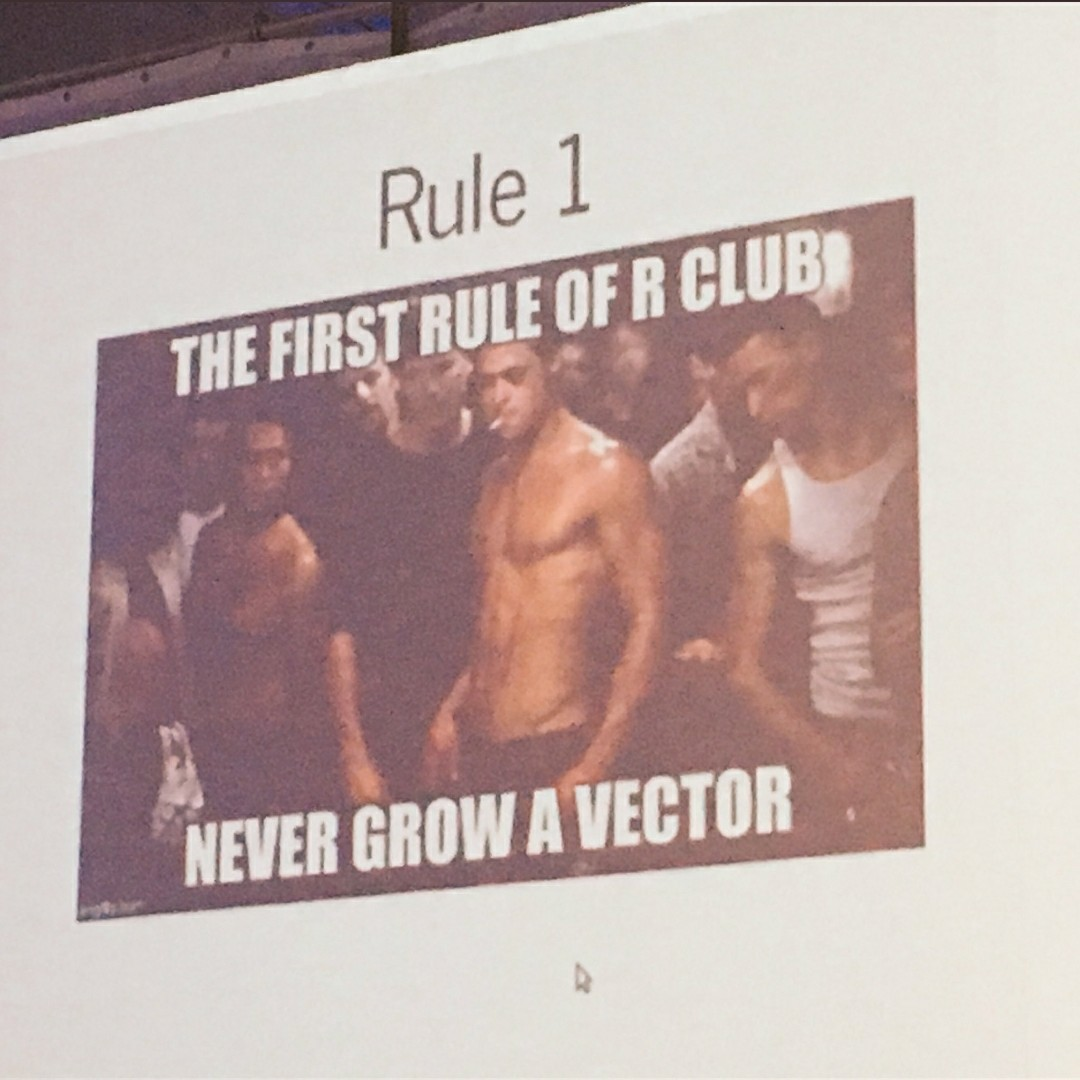
\includegraphics[width=0.9\linewidth]{img/R_club} \end{center}

Voltando ao exemplo das notas, por exemplo, o cálculo da média simples
poderia ser feita diretamente com a função \texttt{apply()}

\begin{Shaded}
\begin{Highlighting}[]
\NormalTok{notas}\OperatorTok{$}\NormalTok{media.apply <-}\StringTok{ }\KeywordTok{apply}\NormalTok{(}\DataTypeTok{X =}\NormalTok{ notas[, provas], }\DataTypeTok{MARGIN =} \DecValTok{1}\NormalTok{, }\DataTypeTok{FUN =}\NormalTok{ mean)}
\KeywordTok{head}\NormalTok{(notas)}
\NormalTok{     nome prova1 prova2 prova3    media   media2   media3        CV  MP}
\DecValTok{1}\NormalTok{ Aluno_}\DecValTok{1}      \DecValTok{8}      \DecValTok{4}      \DecValTok{1} \FloatTok{4.333333} \FloatTok{4.333333} \FloatTok{4.333333} \FloatTok{0.8104349} \FloatTok{4.0}
\DecValTok{2}\NormalTok{ Aluno_}\DecValTok{2}      \DecValTok{2}      \DecValTok{7}      \DecValTok{6} \FloatTok{5.000000} \FloatTok{5.000000} \FloatTok{5.000000} \FloatTok{0.5291503} \FloatTok{5.1}
\DecValTok{3}\NormalTok{ Aluno_}\DecValTok{3}      \DecValTok{9}      \DecValTok{2}      \DecValTok{4} \FloatTok{5.000000} \FloatTok{5.000000} \FloatTok{5.000000} \FloatTok{0.7211103} \FloatTok{4.9}
\DecValTok{4}\NormalTok{ Aluno_}\DecValTok{4}      \DecValTok{1}     \DecValTok{10}      \DecValTok{9} \FloatTok{6.666667} \FloatTok{6.666667} \FloatTok{6.666667} \FloatTok{0.7399324} \FloatTok{6.9}
\DecValTok{5}\NormalTok{ Aluno_}\DecValTok{5}      \DecValTok{7}      \DecValTok{6}      \DecValTok{8} \FloatTok{7.000000} \FloatTok{7.000000} \FloatTok{7.000000} \FloatTok{0.1428571} \FloatTok{7.1}
\DecValTok{6}\NormalTok{ Aluno_}\DecValTok{6}     \DecValTok{10}      \DecValTok{0}      \DecValTok{3} \FloatTok{4.333333} \FloatTok{4.333333} \FloatTok{4.333333} \FloatTok{1.1842157} \FloatTok{4.2}
\NormalTok{       MP2  situacao media.apply}
\DecValTok{1} \FloatTok{4.333333}\NormalTok{ reprovado    }\FloatTok{4.333333}
\DecValTok{2} \FloatTok{5.000000}\NormalTok{ reprovado    }\FloatTok{5.000000}
\DecValTok{3} \FloatTok{5.000000}\NormalTok{ reprovado    }\FloatTok{5.000000}
\DecValTok{4} \FloatTok{6.666667}\NormalTok{ reprovado    }\FloatTok{6.666667}
\DecValTok{5} \FloatTok{7.000000}\NormalTok{  aprovado    }\FloatTok{7.000000}
\DecValTok{6} \FloatTok{4.333333}\NormalTok{ reprovado    }\FloatTok{4.333333}
\end{Highlighting}
\end{Shaded}

As médias ponderadas poderiam ser calculadas da mesma forma, e usando a
função que criamos anteriormente

\begin{Shaded}
\begin{Highlighting}[]
\NormalTok{notas}\OperatorTok{$}\NormalTok{MP.apply <-}\StringTok{ }\KeywordTok{apply}\NormalTok{(}\DataTypeTok{X =}\NormalTok{ notas[, provas], }\DataTypeTok{MARGIN =} \DecValTok{1}\NormalTok{, }\DataTypeTok{FUN =}\NormalTok{ med.pond)}
\KeywordTok{head}\NormalTok{(notas)}
\NormalTok{     nome prova1 prova2 prova3    media   media2   media3        CV  MP}
\DecValTok{1}\NormalTok{ Aluno_}\DecValTok{1}      \DecValTok{8}      \DecValTok{4}      \DecValTok{1} \FloatTok{4.333333} \FloatTok{4.333333} \FloatTok{4.333333} \FloatTok{0.8104349} \FloatTok{4.0}
\DecValTok{2}\NormalTok{ Aluno_}\DecValTok{2}      \DecValTok{2}      \DecValTok{7}      \DecValTok{6} \FloatTok{5.000000} \FloatTok{5.000000} \FloatTok{5.000000} \FloatTok{0.5291503} \FloatTok{5.1}
\DecValTok{3}\NormalTok{ Aluno_}\DecValTok{3}      \DecValTok{9}      \DecValTok{2}      \DecValTok{4} \FloatTok{5.000000} \FloatTok{5.000000} \FloatTok{5.000000} \FloatTok{0.7211103} \FloatTok{4.9}
\DecValTok{4}\NormalTok{ Aluno_}\DecValTok{4}      \DecValTok{1}     \DecValTok{10}      \DecValTok{9} \FloatTok{6.666667} \FloatTok{6.666667} \FloatTok{6.666667} \FloatTok{0.7399324} \FloatTok{6.9}
\DecValTok{5}\NormalTok{ Aluno_}\DecValTok{5}      \DecValTok{7}      \DecValTok{6}      \DecValTok{8} \FloatTok{7.000000} \FloatTok{7.000000} \FloatTok{7.000000} \FloatTok{0.1428571} \FloatTok{7.1}
\DecValTok{6}\NormalTok{ Aluno_}\DecValTok{6}     \DecValTok{10}      \DecValTok{0}      \DecValTok{3} \FloatTok{4.333333} \FloatTok{4.333333} \FloatTok{4.333333} \FloatTok{1.1842157} \FloatTok{4.2}
\NormalTok{       MP2  situacao media.apply MP.apply}
\DecValTok{1} \FloatTok{4.333333}\NormalTok{ reprovado    }\FloatTok{4.333333} \FloatTok{4.333333}
\DecValTok{2} \FloatTok{5.000000}\NormalTok{ reprovado    }\FloatTok{5.000000} \FloatTok{5.000000}
\DecValTok{3} \FloatTok{5.000000}\NormalTok{ reprovado    }\FloatTok{5.000000} \FloatTok{5.000000}
\DecValTok{4} \FloatTok{6.666667}\NormalTok{ reprovado    }\FloatTok{6.666667} \FloatTok{6.666667}
\DecValTok{5} \FloatTok{7.000000}\NormalTok{  aprovado    }\FloatTok{7.000000} \FloatTok{7.000000}
\DecValTok{6} \FloatTok{4.333333}\NormalTok{ reprovado    }\FloatTok{4.333333} \FloatTok{4.333333}
\end{Highlighting}
\end{Shaded}

Mas note que como temos o argumento \texttt{pesos} especificado com um
padrão, devemos alterar na própria função \texttt{apply()}

\begin{Shaded}
\begin{Highlighting}[]
\NormalTok{notas}\OperatorTok{$}\NormalTok{MP.apply <-}\StringTok{ }\KeywordTok{apply}\NormalTok{(}\DataTypeTok{X =}\NormalTok{ notas[, provas], }\DataTypeTok{MARGIN =} \DecValTok{1}\NormalTok{,}
                        \DataTypeTok{FUN =}\NormalTok{ med.pond, }\DataTypeTok{pesos =} \KeywordTok{c}\NormalTok{(}\DecValTok{3}\NormalTok{, }\DecValTok{3}\NormalTok{, }\DecValTok{4}\NormalTok{))}
\KeywordTok{head}\NormalTok{(notas)}
\NormalTok{     nome prova1 prova2 prova3    media   media2   media3        CV  MP}
\DecValTok{1}\NormalTok{ Aluno_}\DecValTok{1}      \DecValTok{8}      \DecValTok{4}      \DecValTok{1} \FloatTok{4.333333} \FloatTok{4.333333} \FloatTok{4.333333} \FloatTok{0.8104349} \FloatTok{4.0}
\DecValTok{2}\NormalTok{ Aluno_}\DecValTok{2}      \DecValTok{2}      \DecValTok{7}      \DecValTok{6} \FloatTok{5.000000} \FloatTok{5.000000} \FloatTok{5.000000} \FloatTok{0.5291503} \FloatTok{5.1}
\DecValTok{3}\NormalTok{ Aluno_}\DecValTok{3}      \DecValTok{9}      \DecValTok{2}      \DecValTok{4} \FloatTok{5.000000} \FloatTok{5.000000} \FloatTok{5.000000} \FloatTok{0.7211103} \FloatTok{4.9}
\DecValTok{4}\NormalTok{ Aluno_}\DecValTok{4}      \DecValTok{1}     \DecValTok{10}      \DecValTok{9} \FloatTok{6.666667} \FloatTok{6.666667} \FloatTok{6.666667} \FloatTok{0.7399324} \FloatTok{6.9}
\DecValTok{5}\NormalTok{ Aluno_}\DecValTok{5}      \DecValTok{7}      \DecValTok{6}      \DecValTok{8} \FloatTok{7.000000} \FloatTok{7.000000} \FloatTok{7.000000} \FloatTok{0.1428571} \FloatTok{7.1}
\DecValTok{6}\NormalTok{ Aluno_}\DecValTok{6}     \DecValTok{10}      \DecValTok{0}      \DecValTok{3} \FloatTok{4.333333} \FloatTok{4.333333} \FloatTok{4.333333} \FloatTok{1.1842157} \FloatTok{4.2}
\NormalTok{       MP2  situacao media.apply MP.apply}
\DecValTok{1} \FloatTok{4.333333}\NormalTok{ reprovado    }\FloatTok{4.333333}      \FloatTok{4.0}
\DecValTok{2} \FloatTok{5.000000}\NormalTok{ reprovado    }\FloatTok{5.000000}      \FloatTok{5.1}
\DecValTok{3} \FloatTok{5.000000}\NormalTok{ reprovado    }\FloatTok{5.000000}      \FloatTok{4.9}
\DecValTok{4} \FloatTok{6.666667}\NormalTok{ reprovado    }\FloatTok{6.666667}      \FloatTok{6.9}
\DecValTok{5} \FloatTok{7.000000}\NormalTok{  aprovado    }\FloatTok{7.000000}      \FloatTok{7.1}
\DecValTok{6} \FloatTok{4.333333}\NormalTok{ reprovado    }\FloatTok{4.333333}      \FloatTok{4.2}
\end{Highlighting}
\end{Shaded}

NOTA: veja que isso é possível devido à presença do argumento
\texttt{...} na função \texttt{apply()}, que permite passar argumentos
de outras funções dentro dela.

Também poderíamos usar a função \texttt{weighted.mean()} implementada no
R

\begin{Shaded}
\begin{Highlighting}[]
\NormalTok{notas}\OperatorTok{$}\NormalTok{MP2.apply <-}\StringTok{ }\KeywordTok{apply}\NormalTok{(}\DataTypeTok{X =}\NormalTok{ notas[, provas], }\DataTypeTok{MARGIN =} \DecValTok{1}\NormalTok{,}
                         \DataTypeTok{FUN =}\NormalTok{ weighted.mean, }\DataTypeTok{w =} \KeywordTok{c}\NormalTok{(}\DecValTok{3}\NormalTok{, }\DecValTok{3}\NormalTok{, }\DecValTok{4}\NormalTok{))}
\KeywordTok{head}\NormalTok{(notas)}
\NormalTok{     nome prova1 prova2 prova3    media   media2   media3        CV  MP}
\DecValTok{1}\NormalTok{ Aluno_}\DecValTok{1}      \DecValTok{8}      \DecValTok{4}      \DecValTok{1} \FloatTok{4.333333} \FloatTok{4.333333} \FloatTok{4.333333} \FloatTok{0.8104349} \FloatTok{4.0}
\DecValTok{2}\NormalTok{ Aluno_}\DecValTok{2}      \DecValTok{2}      \DecValTok{7}      \DecValTok{6} \FloatTok{5.000000} \FloatTok{5.000000} \FloatTok{5.000000} \FloatTok{0.5291503} \FloatTok{5.1}
\DecValTok{3}\NormalTok{ Aluno_}\DecValTok{3}      \DecValTok{9}      \DecValTok{2}      \DecValTok{4} \FloatTok{5.000000} \FloatTok{5.000000} \FloatTok{5.000000} \FloatTok{0.7211103} \FloatTok{4.9}
\DecValTok{4}\NormalTok{ Aluno_}\DecValTok{4}      \DecValTok{1}     \DecValTok{10}      \DecValTok{9} \FloatTok{6.666667} \FloatTok{6.666667} \FloatTok{6.666667} \FloatTok{0.7399324} \FloatTok{6.9}
\DecValTok{5}\NormalTok{ Aluno_}\DecValTok{5}      \DecValTok{7}      \DecValTok{6}      \DecValTok{8} \FloatTok{7.000000} \FloatTok{7.000000} \FloatTok{7.000000} \FloatTok{0.1428571} \FloatTok{7.1}
\DecValTok{6}\NormalTok{ Aluno_}\DecValTok{6}     \DecValTok{10}      \DecValTok{0}      \DecValTok{3} \FloatTok{4.333333} \FloatTok{4.333333} \FloatTok{4.333333} \FloatTok{1.1842157} \FloatTok{4.2}
\NormalTok{       MP2  situacao media.apply MP.apply MP2.apply}
\DecValTok{1} \FloatTok{4.333333}\NormalTok{ reprovado    }\FloatTok{4.333333}      \FloatTok{4.0}       \FloatTok{4.0}
\DecValTok{2} \FloatTok{5.000000}\NormalTok{ reprovado    }\FloatTok{5.000000}      \FloatTok{5.1}       \FloatTok{5.1}
\DecValTok{3} \FloatTok{5.000000}\NormalTok{ reprovado    }\FloatTok{5.000000}      \FloatTok{4.9}       \FloatTok{4.9}
\DecValTok{4} \FloatTok{6.666667}\NormalTok{ reprovado    }\FloatTok{6.666667}      \FloatTok{6.9}       \FloatTok{6.9}
\DecValTok{5} \FloatTok{7.000000}\NormalTok{  aprovado    }\FloatTok{7.000000}      \FloatTok{7.1}       \FloatTok{7.1}
\DecValTok{6} \FloatTok{4.333333}\NormalTok{ reprovado    }\FloatTok{4.333333}      \FloatTok{4.2}       \FloatTok{4.2}
\end{Highlighting}
\end{Shaded}

O Coeficiente de Variação poderia ser calculado usando nossa função
\texttt{cv()}

\begin{Shaded}
\begin{Highlighting}[]
\NormalTok{notas}\OperatorTok{$}\NormalTok{CV.apply <-}\StringTok{ }\KeywordTok{apply}\NormalTok{(}\DataTypeTok{X =}\NormalTok{ notas[, provas], }\DataTypeTok{MARGIN =} \DecValTok{1}\NormalTok{, }\DataTypeTok{FUN =}\NormalTok{ cv)}
\KeywordTok{head}\NormalTok{(notas)}
\NormalTok{     nome prova1 prova2 prova3    media   media2   media3        CV  MP}
\DecValTok{1}\NormalTok{ Aluno_}\DecValTok{1}      \DecValTok{8}      \DecValTok{4}      \DecValTok{1} \FloatTok{4.333333} \FloatTok{4.333333} \FloatTok{4.333333} \FloatTok{0.8104349} \FloatTok{4.0}
\DecValTok{2}\NormalTok{ Aluno_}\DecValTok{2}      \DecValTok{2}      \DecValTok{7}      \DecValTok{6} \FloatTok{5.000000} \FloatTok{5.000000} \FloatTok{5.000000} \FloatTok{0.5291503} \FloatTok{5.1}
\DecValTok{3}\NormalTok{ Aluno_}\DecValTok{3}      \DecValTok{9}      \DecValTok{2}      \DecValTok{4} \FloatTok{5.000000} \FloatTok{5.000000} \FloatTok{5.000000} \FloatTok{0.7211103} \FloatTok{4.9}
\DecValTok{4}\NormalTok{ Aluno_}\DecValTok{4}      \DecValTok{1}     \DecValTok{10}      \DecValTok{9} \FloatTok{6.666667} \FloatTok{6.666667} \FloatTok{6.666667} \FloatTok{0.7399324} \FloatTok{6.9}
\DecValTok{5}\NormalTok{ Aluno_}\DecValTok{5}      \DecValTok{7}      \DecValTok{6}      \DecValTok{8} \FloatTok{7.000000} \FloatTok{7.000000} \FloatTok{7.000000} \FloatTok{0.1428571} \FloatTok{7.1}
\DecValTok{6}\NormalTok{ Aluno_}\DecValTok{6}     \DecValTok{10}      \DecValTok{0}      \DecValTok{3} \FloatTok{4.333333} \FloatTok{4.333333} \FloatTok{4.333333} \FloatTok{1.1842157} \FloatTok{4.2}
\NormalTok{       MP2  situacao media.apply MP.apply MP2.apply  CV.apply}
\DecValTok{1} \FloatTok{4.333333}\NormalTok{ reprovado    }\FloatTok{4.333333}      \FloatTok{4.0}       \FloatTok{4.0} \FloatTok{0.8104349}
\DecValTok{2} \FloatTok{5.000000}\NormalTok{ reprovado    }\FloatTok{5.000000}      \FloatTok{5.1}       \FloatTok{5.1} \FloatTok{0.5291503}
\DecValTok{3} \FloatTok{5.000000}\NormalTok{ reprovado    }\FloatTok{5.000000}      \FloatTok{4.9}       \FloatTok{4.9} \FloatTok{0.7211103}
\DecValTok{4} \FloatTok{6.666667}\NormalTok{ reprovado    }\FloatTok{6.666667}      \FloatTok{6.9}       \FloatTok{6.9} \FloatTok{0.7399324}
\DecValTok{5} \FloatTok{7.000000}\NormalTok{  aprovado    }\FloatTok{7.000000}      \FloatTok{7.1}       \FloatTok{7.1} \FloatTok{0.1428571}
\DecValTok{6} \FloatTok{4.333333}\NormalTok{ reprovado    }\FloatTok{4.333333}      \FloatTok{4.2}       \FloatTok{4.2} \FloatTok{1.1842157}
\end{Highlighting}
\end{Shaded}

Finalmente, a estrutura de repetição \texttt{if()} também possui uma
forma vetorizada através da função \texttt{ifelse()}. Essa função
funciona da seguinte forma:

\begin{Shaded}
\begin{Highlighting}[]
\KeywordTok{ifelse}\NormalTok{(}\OperatorTok{<}\NormalTok{condição}\OperatorTok{>}\NormalTok{, }\OperatorTok{<}\NormalTok{valor se verdadeiro}\OperatorTok{>}\NormalTok{, }\OperatorTok{<}\NormalTok{valor se falso}\OperatorTok{>}\NormalTok{)}
\end{Highlighting}
\end{Shaded}

Dessa forma, a atribuição da situação dos alunos poderia ser feita da
seguinte forma:

\begin{Shaded}
\begin{Highlighting}[]
\NormalTok{notas}\OperatorTok{$}\NormalTok{situacao2 <-}\StringTok{ }\KeywordTok{ifelse}\NormalTok{(notas}\OperatorTok{$}\NormalTok{MP }\OperatorTok{>=}\StringTok{ }\DecValTok{7}\NormalTok{, }\StringTok{"aprovado"}\NormalTok{, }\StringTok{"reprovado"}\NormalTok{)}
\KeywordTok{head}\NormalTok{(notas)}
\NormalTok{     nome prova1 prova2 prova3    media   media2   media3        CV  MP}
\DecValTok{1}\NormalTok{ Aluno_}\DecValTok{1}      \DecValTok{8}      \DecValTok{4}      \DecValTok{1} \FloatTok{4.333333} \FloatTok{4.333333} \FloatTok{4.333333} \FloatTok{0.8104349} \FloatTok{4.0}
\DecValTok{2}\NormalTok{ Aluno_}\DecValTok{2}      \DecValTok{2}      \DecValTok{7}      \DecValTok{6} \FloatTok{5.000000} \FloatTok{5.000000} \FloatTok{5.000000} \FloatTok{0.5291503} \FloatTok{5.1}
\DecValTok{3}\NormalTok{ Aluno_}\DecValTok{3}      \DecValTok{9}      \DecValTok{2}      \DecValTok{4} \FloatTok{5.000000} \FloatTok{5.000000} \FloatTok{5.000000} \FloatTok{0.7211103} \FloatTok{4.9}
\DecValTok{4}\NormalTok{ Aluno_}\DecValTok{4}      \DecValTok{1}     \DecValTok{10}      \DecValTok{9} \FloatTok{6.666667} \FloatTok{6.666667} \FloatTok{6.666667} \FloatTok{0.7399324} \FloatTok{6.9}
\DecValTok{5}\NormalTok{ Aluno_}\DecValTok{5}      \DecValTok{7}      \DecValTok{6}      \DecValTok{8} \FloatTok{7.000000} \FloatTok{7.000000} \FloatTok{7.000000} \FloatTok{0.1428571} \FloatTok{7.1}
\DecValTok{6}\NormalTok{ Aluno_}\DecValTok{6}     \DecValTok{10}      \DecValTok{0}      \DecValTok{3} \FloatTok{4.333333} \FloatTok{4.333333} \FloatTok{4.333333} \FloatTok{1.1842157} \FloatTok{4.2}
\NormalTok{       MP2  situacao media.apply MP.apply MP2.apply  CV.apply situacao2}
\DecValTok{1} \FloatTok{4.333333}\NormalTok{ reprovado    }\FloatTok{4.333333}      \FloatTok{4.0}       \FloatTok{4.0} \FloatTok{0.8104349}\NormalTok{ reprovado}
\DecValTok{2} \FloatTok{5.000000}\NormalTok{ reprovado    }\FloatTok{5.000000}      \FloatTok{5.1}       \FloatTok{5.1} \FloatTok{0.5291503}\NormalTok{ reprovado}
\DecValTok{3} \FloatTok{5.000000}\NormalTok{ reprovado    }\FloatTok{5.000000}      \FloatTok{4.9}       \FloatTok{4.9} \FloatTok{0.7211103}\NormalTok{ reprovado}
\DecValTok{4} \FloatTok{6.666667}\NormalTok{ reprovado    }\FloatTok{6.666667}      \FloatTok{6.9}       \FloatTok{6.9} \FloatTok{0.7399324}\NormalTok{ reprovado}
\DecValTok{5} \FloatTok{7.000000}\NormalTok{  aprovado    }\FloatTok{7.000000}      \FloatTok{7.1}       \FloatTok{7.1} \FloatTok{0.1428571}\NormalTok{  aprovado}
\DecValTok{6} \FloatTok{4.333333}\NormalTok{ reprovado    }\FloatTok{4.333333}      \FloatTok{4.2}       \FloatTok{4.2} \FloatTok{1.1842157}\NormalTok{ reprovado}
\end{Highlighting}
\end{Shaded}

\section{Outras estruturas: while e
repeat}\label{outras-estruturas-while-e-repeat}

O \texttt{while} executa comandos enquanto uma determinada condição
permanece verdadeira.

\begin{Shaded}
\begin{Highlighting}[]
\NormalTok{## Calcule a soma em 1,2,3... até que o soma seja maior do que 1000}
\NormalTok{n <-}\StringTok{ }\DecValTok{0}
\NormalTok{soma <-}\StringTok{ }\DecValTok{0}
\ControlFlowTok{while}\NormalTok{(soma }\OperatorTok{<=}\StringTok{ }\DecValTok{1000}\NormalTok{)\{}
\NormalTok{    n <-}\StringTok{ }\NormalTok{n }\OperatorTok{+}\StringTok{ }\DecValTok{1}
\NormalTok{    soma <-}\StringTok{ }\NormalTok{soma }\OperatorTok{+}\StringTok{ }\NormalTok{n}
\NormalTok{\}}
\NormalTok{soma}
\NormalTok{[}\DecValTok{1}\NormalTok{] }\DecValTok{1035}
\end{Highlighting}
\end{Shaded}

O \texttt{repeat} é ainda mais básico, e irá executar comandos até que
você explicitamente pare a execução com o comando \texttt{break}.

\begin{Shaded}
\begin{Highlighting}[]
\NormalTok{## Mesmo exemplo}
\NormalTok{n <-}\StringTok{ }\DecValTok{0}
\NormalTok{soma <-}\StringTok{ }\DecValTok{0}
\ControlFlowTok{repeat}\NormalTok{\{}
\NormalTok{    n <-}\StringTok{ }\NormalTok{n }\OperatorTok{+}\StringTok{ }\DecValTok{1}
\NormalTok{    soma <-}\StringTok{ }\NormalTok{soma }\OperatorTok{+}\StringTok{ }\NormalTok{n}
    \ControlFlowTok{if}\NormalTok{(soma }\OperatorTok{>}\StringTok{ }\DecValTok{1000}\NormalTok{) }\ControlFlowTok{break}
\NormalTok{\}}
\NormalTok{soma}
\NormalTok{[}\DecValTok{1}\NormalTok{] }\DecValTok{1035}
\end{Highlighting}
\end{Shaded}

\appendix


\chapter{Programação Orientada a
Objetos}\label{programacao-orientada-a-objetos}

Como vimos anteriormente, o R é uma linguagem de programação orientada à
objetos. Dois conceitos fundamentais desse tipo de linguagem são os de
\textbf{classe} e \textbf{método}. Já vimos também que todo objeto no R
possui uma classe (que define sua estrutura) e analisamos algumas delas.
O que seria então um método? Para responder essa pergunta precisamos
entender inicialmente os tipos de orientação a objetos que o R possui.

O R possui 3 sitemas de orientação a objetos: \textbf{S3}, \textbf{S4},
e \textbf{RC}:

\begin{itemize}
\tightlist
\item
  \textbf{S3}: implementa um estilo de programação orientada a objeto
  chamada de \emph{generic-function}. Esse é o estilo mais básico de
  programação em R (e também o mais utilizado). A ideia é que existam
  \textbf{funções genéricas} que decidem qual método aplicar de acordo
  com a classe do objeto. Os métodos são definidos da mesma forma que
  qualquer função, mas chamados de amenira diferente. É um estilo de
  programação mais ``informal'', mas possibilita uma grande liberdade
  para o programador.
\item
  \textbf{S4}: é um estilo mais formal, no sentido que que as funções
  genéricas devem possuir uma classe formal definida. Além disso, é
  possível também fazer o \textbf{despacho múltiplo de métodos}, ao
  contrário da classe S3.
\item
  \textbf{RC}: (\emph{Reference Classes}, antes chamado de R5) é o
  sistema mais novo implementado no R. A principal diferença com os
  sistemas S3 e S4 é que métodos pertencem à objetos, não à funções.
  Isso faz com que objetos da classe RC se comportem mais como objetos
  da maioria das linguagens de programação, como Python, Java, e C\#.
\end{itemize}

Nesta sessão vamos abordar como funcionam os métodos como definidos pelo
sistema S3, por ser o mais utilizado na prática para se criar novas
funções no R. Para saber mais sobre os outros métodos, consulte o livro
\href{http://adv-r.had.co.nz/OO-essentials.html}{Advanced R}.

Vamos entender como uma função genérica pode ser criada através de um
exemplo. Usando a função \texttt{methods()}, podemos verificar quais
métodos estão disponíveis para uma determinada função, por exemplo, para
a função \texttt{mean()}:

\begin{Shaded}
\begin{Highlighting}[]
\KeywordTok{methods}\NormalTok{(mean)}
\NormalTok{[}\DecValTok{1}\NormalTok{] mean.Date     mean.default  mean.difftime mean.POSIXct  mean.POSIXlt }
\NormalTok{see }\StringTok{'?methods'} \ControlFlowTok{for}\NormalTok{ accessing help and source code}
\end{Highlighting}
\end{Shaded}

O resultado são expressões do tipo
\texttt{mean.\textless{}classe\textgreater{}}, onde
\texttt{\textless{}classe\textgreater{}} é uma classe de objeto como
aquelas vistas anteriormente. Isso significa que a função
\texttt{mean()}, quando aplicada à um objeto da classe \texttt{Date},
por exemplo, pode ter um comportamento diferente quando a mesma função
for aplicada à um objeto de outra classe (numérica).

Suponha que temos o seguinte vetor numérico:

\begin{Shaded}
\begin{Highlighting}[]
\KeywordTok{set.seed}\NormalTok{(}\DecValTok{1}\NormalTok{)}
\NormalTok{vec <-}\StringTok{ }\KeywordTok{rnorm}\NormalTok{(}\DecValTok{100}\NormalTok{)}
\KeywordTok{class}\NormalTok{(vec)}
\NormalTok{[}\DecValTok{1}\NormalTok{] }\StringTok{"numeric"}
\end{Highlighting}
\end{Shaded}

e queremos calcular sua média. Basta aplicar a função \texttt{mean()}
nesse objeto para obtermos o resultado esperado

\begin{Shaded}
\begin{Highlighting}[]
\KeywordTok{mean}\NormalTok{(vec)}
\NormalTok{[}\DecValTok{1}\NormalTok{] }\FloatTok{0.1088874}
\end{Highlighting}
\end{Shaded}

Mas isso só é possível porque existe um método definido espcificamente
para um vetor da classe \texttt{numeric}, que nesse caso é a função
\texttt{mean.default}. A função genérica nesse caso é a \texttt{mean()},
e a função método é a \texttt{mean.default}. Veja que não precisamos
escrever onome inteiro da função genérica para que ela seja utilizada,
como por exemplo,

\begin{Shaded}
\begin{Highlighting}[]
\KeywordTok{mean.default}\NormalTok{(vec)}
\NormalTok{[}\DecValTok{1}\NormalTok{] }\FloatTok{0.1088874}
\end{Highlighting}
\end{Shaded}

Uma vez passado um objeto para uma função, é a classe do objeto que irá
definir qual método utilizar, de acordo com os métodos disponíveis. Veja
o que acontece se forcarmos o uso da função \texttt{mean.Date()} nesse
vetor

\begin{Shaded}
\begin{Highlighting}[]
\KeywordTok{mean.Date}\NormalTok{(vec)}
\NormalTok{[}\DecValTok{1}\NormalTok{] }\StringTok{"1970-01-01"}
\end{Highlighting}
\end{Shaded}

O resultado não faz sentido pois ele é específico para um objeto da
classe \texttt{Date}.

Tudo isso acontece por causa de um mecanismo chamado de \textbf{despacho
de métodos} (\emph{method dispatch}), que é responsável por identificar
a classe do objeto e utilizar (``despachar'') a função método correta
para aquela classe. Toda função genérica possui a mesma forma: uma
chamada para a função \texttt{UseMethod()}, que especifica o nome
genérico e o objeto a ser despachado. Por exemplo, veja o código fonte
da função \texttt{mean()}

\begin{Shaded}
\begin{Highlighting}[]
\NormalTok{mean}
\ControlFlowTok{function}\NormalTok{ (x, ...) }
\KeywordTok{UseMethod}\NormalTok{(}\StringTok{"mean"}\NormalTok{)}
\OperatorTok{<}\NormalTok{bytecode}\OperatorTok{:}\StringTok{ }\DecValTok{0x7bc0100}\OperatorTok{>}
\ErrorTok{<}\NormalTok{environment}\OperatorTok{:}\StringTok{ }\NormalTok{namespace}\OperatorTok{:}\NormalTok{base}\OperatorTok{>}
\end{Highlighting}
\end{Shaded}

Agora veja o código fonte da função \texttt{mean.default}, que é o
método específico para vetores numéricos

\begin{Shaded}
\begin{Highlighting}[]
\NormalTok{mean.default}
\ControlFlowTok{function}\NormalTok{ (x, }\DataTypeTok{trim =} \DecValTok{0}\NormalTok{, }\DataTypeTok{na.rm =} \OtherTok{FALSE}\NormalTok{, ...) }
\NormalTok{\{}
    \ControlFlowTok{if}\NormalTok{ (}\OperatorTok{!}\KeywordTok{is.numeric}\NormalTok{(x) }\OperatorTok{&&}\StringTok{ }\OperatorTok{!}\KeywordTok{is.complex}\NormalTok{(x) }\OperatorTok{&&}\StringTok{ }\OperatorTok{!}\KeywordTok{is.logical}\NormalTok{(x)) \{}
        \KeywordTok{warning}\NormalTok{(}\StringTok{"argument is not numeric or logical: returning NA"}\NormalTok{)}
        \KeywordTok{return}\NormalTok{(}\OtherTok{NA_real_}\NormalTok{)}
\NormalTok{    \}}
    \ControlFlowTok{if}\NormalTok{ (na.rm) }
\NormalTok{        x <-}\StringTok{ }\NormalTok{x[}\OperatorTok{!}\KeywordTok{is.na}\NormalTok{(x)]}
    \ControlFlowTok{if}\NormalTok{ (}\OperatorTok{!}\KeywordTok{is.numeric}\NormalTok{(trim) }\OperatorTok{||}\StringTok{ }\KeywordTok{length}\NormalTok{(trim) }\OperatorTok{!=}\StringTok{ }\NormalTok{1L) }
        \KeywordTok{stop}\NormalTok{(}\StringTok{"'trim' must be numeric of length one"}\NormalTok{)}
\NormalTok{    n <-}\StringTok{ }\KeywordTok{length}\NormalTok{(x)}
    \ControlFlowTok{if}\NormalTok{ (trim }\OperatorTok{>}\StringTok{ }\DecValTok{0} \OperatorTok{&&}\StringTok{ }\NormalTok{n) \{}
        \ControlFlowTok{if}\NormalTok{ (}\KeywordTok{is.complex}\NormalTok{(x)) }
            \KeywordTok{stop}\NormalTok{(}\StringTok{"trimmed means are not defined for complex data"}\NormalTok{)}
        \ControlFlowTok{if}\NormalTok{ (}\KeywordTok{anyNA}\NormalTok{(x)) }
            \KeywordTok{return}\NormalTok{(}\OtherTok{NA_real_}\NormalTok{)}
        \ControlFlowTok{if}\NormalTok{ (trim }\OperatorTok{>=}\StringTok{ }\FloatTok{0.5}\NormalTok{) }
            \KeywordTok{return}\NormalTok{(stats}\OperatorTok{::}\KeywordTok{median}\NormalTok{(x, }\DataTypeTok{na.rm =} \OtherTok{FALSE}\NormalTok{))}
\NormalTok{        lo <-}\StringTok{ }\KeywordTok{floor}\NormalTok{(n }\OperatorTok{*}\StringTok{ }\NormalTok{trim) }\OperatorTok{+}\StringTok{ }\DecValTok{1}
\NormalTok{        hi <-}\StringTok{ }\NormalTok{n }\OperatorTok{+}\StringTok{ }\DecValTok{1} \OperatorTok{-}\StringTok{ }\NormalTok{lo}
\NormalTok{        x <-}\StringTok{ }\KeywordTok{sort.int}\NormalTok{(x, }\DataTypeTok{partial =} \KeywordTok{unique}\NormalTok{(}\KeywordTok{c}\NormalTok{(lo, hi)))[lo}\OperatorTok{:}\NormalTok{hi]}
\NormalTok{    \}}
    \KeywordTok{.Internal}\NormalTok{(}\KeywordTok{mean}\NormalTok{(x))}
\NormalTok{\}}
\OperatorTok{<}\NormalTok{bytecode}\OperatorTok{:}\StringTok{ }\DecValTok{0x7bbf6b8}\OperatorTok{>}
\ErrorTok{<}\NormalTok{environment}\OperatorTok{:}\StringTok{ }\NormalTok{namespace}\OperatorTok{:}\NormalTok{base}\OperatorTok{>}
\end{Highlighting}
\end{Shaded}

Agora suponha que você ddeseja criar uma função que calcule a média para
um objeto de uma classe diferente daquelas previamente definidas. Por
exemplo, suponha que você quer que a função \texttt{mean()} retorne a
média das linhas de uma matriz.

\begin{Shaded}
\begin{Highlighting}[]
\KeywordTok{set.seed}\NormalTok{(}\DecValTok{1}\NormalTok{)}
\NormalTok{mat <-}\StringTok{ }\KeywordTok{matrix}\NormalTok{(}\KeywordTok{rnorm}\NormalTok{(}\DecValTok{50}\NormalTok{), }\DataTypeTok{nrow =} \DecValTok{5}\NormalTok{)}
\KeywordTok{mean}\NormalTok{(mat)}
\NormalTok{[}\DecValTok{1}\NormalTok{] }\FloatTok{0.1004483}
\end{Highlighting}
\end{Shaded}

O resultado é a média de todos os elementos, e não de cada linha. Nesse
caso, podemos definir nossa própria função método para fazer o cálculo
que precisamos. Por exemplo:

\begin{Shaded}
\begin{Highlighting}[]
\NormalTok{mean.matrix <-}\StringTok{ }\ControlFlowTok{function}\NormalTok{(x, ...) }\KeywordTok{rowMeans}\NormalTok{(x)}
\end{Highlighting}
\end{Shaded}

Uma função método é sempre definida dessa forma:
\texttt{\textless{}funçãogenérica\textgreater{}.\textless{}classe\textgreater{}}.
Agora podemos ver novamente os métodos disponíveis para a função
\texttt{mean()}

\begin{Shaded}
\begin{Highlighting}[]
\KeywordTok{methods}\NormalTok{(mean)}
\NormalTok{[}\DecValTok{1}\NormalTok{] mean.Date     mean.default  mean.difftime mean.matrix   mean.POSIXct }
\NormalTok{[}\DecValTok{6}\NormalTok{] mean.POSIXlt }
\NormalTok{see }\StringTok{'?methods'} \ControlFlowTok{for}\NormalTok{ accessing help and source code}
\end{Highlighting}
\end{Shaded}

e simplesmente aplicar a função genérica \texttt{mean()} à um objeto da
classe \texttt{matrix} para obter o resultado que desejamos

\begin{Shaded}
\begin{Highlighting}[]
\KeywordTok{class}\NormalTok{(mat)}
\NormalTok{[}\DecValTok{1}\NormalTok{] }\StringTok{"matrix"}
\KeywordTok{mean}\NormalTok{(mat)}
\NormalTok{[}\DecValTok{1}\NormalTok{]  }\FloatTok{0.09544402}  \FloatTok{0.12852087}  \FloatTok{0.06229588} \OperatorTok{-}\FloatTok{0.01993810}  \FloatTok{0.23591872}
\end{Highlighting}
\end{Shaded}

Esse exemplo ilustra como é simples criar funções método para diferentes
classes de objetos. Poderíamos fazer o mesmo para objetos das classes
\texttt{data.frame} e \texttt{list}

\begin{Shaded}
\begin{Highlighting}[]
\NormalTok{mean.data.frame <-}\StringTok{ }\ControlFlowTok{function}\NormalTok{(x, ...) }\KeywordTok{sapply}\NormalTok{(x, mean, ...)}
\NormalTok{mean.list <-}\StringTok{ }\ControlFlowTok{function}\NormalTok{(x, ...) }\KeywordTok{lapply}\NormalTok{(x, mean)}
\end{Highlighting}
\end{Shaded}

Aplicando em objetos dessas classes específicas, obtemos:

\begin{Shaded}
\begin{Highlighting}[]
\NormalTok{## Data frame}
\KeywordTok{set.seed}\NormalTok{(}\DecValTok{1}\NormalTok{)}
\NormalTok{da <-}\StringTok{ }\KeywordTok{data.frame}\NormalTok{(}\DataTypeTok{c1 =} \KeywordTok{rnorm}\NormalTok{(}\DecValTok{10}\NormalTok{),}
                 \DataTypeTok{c2 =} \KeywordTok{runif}\NormalTok{(}\DecValTok{10}\NormalTok{))}
\KeywordTok{class}\NormalTok{(da)}
\NormalTok{[}\DecValTok{1}\NormalTok{] }\StringTok{"data.frame"}
\KeywordTok{mean}\NormalTok{(da)}
\NormalTok{       c1        c2 }
\FloatTok{0.1322028} \FloatTok{0.4183230} 
\NormalTok{## Lista}
\KeywordTok{set.seed}\NormalTok{(}\DecValTok{1}\NormalTok{)}
\NormalTok{dl <-}\StringTok{ }\KeywordTok{list}\NormalTok{(}\KeywordTok{rnorm}\NormalTok{(}\DecValTok{10}\NormalTok{), }\KeywordTok{runif}\NormalTok{(}\DecValTok{50}\NormalTok{))}
\KeywordTok{class}\NormalTok{(dl)}
\NormalTok{[}\DecValTok{1}\NormalTok{] }\StringTok{"list"}
\KeywordTok{mean}\NormalTok{(dl)}
\NormalTok{[[}\DecValTok{1}\NormalTok{]]}
\NormalTok{[}\DecValTok{1}\NormalTok{] }\FloatTok{0.1322028}

\NormalTok{[[}\DecValTok{2}\NormalTok{]]}
\NormalTok{[}\DecValTok{1}\NormalTok{] }\FloatTok{0.4946632}
\end{Highlighting}
\end{Shaded}

Obviamente esse processo todo é extremamente importante ao se criar
novas funções no R. Podemos tanto criar uma função genérica (como a
\texttt{mean()}) e diversos métodos para ela usando classes de objetos
existentes, quanto (inclusive) criar novas classes e funções método para
elas. Essa é uma das grandes lberdades que o método S3 de orientação à
objetos permite, e possivelmente um dos motivos pelos quais é
relativamente simples criar pacotes inteiros no R.

\end{document}
